\documentclass[12pt]{ociamthesis}  % default square logo 
%\documentclass[12pt,beltcrest]{ociamthesis} % use old belt crest logo
%\documentclass[12pt,shieldcrest]{ociamthesis} % use older shield crest logo

%load any additional packages
\usepackage{amssymb}
\usepackage{listings}

%input macros (i.e. write your own macros file called mymacros.tex 
%and uncomment the next line)
%\include{mymacros}

\title{Modul Praktikum \\[1ex]     %your thesis title,
        Kecerdasan Buatan}   %note \\[1ex] is a line break in the title

\author{Rolly Maulana Awangga}             %your name
\college{0410118609\\[5ex]
Applied Bachelor of Informatics Engineering}  %your college

%\renewcommand{\submittedtext}{change the default text here if needed}
\degree{Politeknik Pos Indonesia}     %the degree
\degreedate{Bandung 2019}         %the degree date

%end the preamble and start the document
\begin{document}

%this baselineskip gives sufficient line spacing for an examiner to easily
%markup the thesis with comments
\baselineskip=18pt plus1pt

%set the number of sectioning levels that get number and appear in the contents
\setcounter{secnumdepth}{3}
\setcounter{tocdepth}{3}


\maketitle                  % create a title page from the preamble info
\begin{dedication}
`Jika Kamu tidak dapat menahan lelahnya belajar, \\
Maka kamu harus sanggup menahan perihnya Kebodohan.'\\ 
~Imam Syafi'i~\\
\end{dedication}        % include a dedication.tex file
\begin{acknowledgements}
Pertama-tama kami panjatkan puji dan syukur kepada Allah SWT yang telah memberikan rahmat dan hidayah-Nya sehingga Buku Pedoman Tingkat Akhir ini dapat diselesaikan.
\end{acknowledgements}   % include an acknowledgements.tex file
\begin{abstract}
	Buku Pedoman ini dibuat dengan tujuan memberikan acuan, bagi mahasiswa Tingkat Akhir dan dosen
	Pembimbing. Pada intinya buku ini menjelaskan secara lengkap tentang Standar pengerjaan Intership  dan 
	Tugas Akhir
	di Program Studi D4 Teknik Informatika, dan juga mengatur mekanisme, teknik penulisan, serta
	penilaiannya.Dengan demikian diharapkan semua pihak yang terlibat dalam aktivitas Bimbingan Mahasiswa Tingkat Akhir
	berjalan lancar dan sesuai dengan standar.
\end{abstract}          % include the abstract

\begin{romanpages}          % start roman page numbering
\tableofcontents            % generate and include a table of contents
\listoffigures              % generate and include a list of figures
\end{romanpages}            % end roman page numbering

%now include the files of latex for each of the chapters etc
\chapter{Mengenal Kecerdasan Buatan dan Scikit-Learn}
Buku umum yang digunakan adalah \cite{russell2016artificial} dan  
untuk sebelum UTS menggunakan buku \textit{Python Artificial Intelligence Projects for Beginners}\cite{eckroth2018python}.
Dengan praktek menggunakan python 3 dan editor anaconda dan library python scikit-learn.
Tujuan pembelajaran pada pertemuan pertama antara lain:
\begin{enumerate}
\item
Mengerti definisi kecerdasan buatan, sejarah kecerdasan buatan, perkembangan dan penggunaan di perusahaan
\item
Memahami cara instalasi dan pemakaian sci-kit learn
\item
Memahami cara penggunaan variabel explorer di spyder
\end{enumerate}
Tugas dengan cara dikumpulkan dengan pull request ke github dengan menggunakan latex pada repo yang dibuat oleh asisten riset.

\section{Teori}
Praktek teori penunjang yang dikerjakan :
\begin{enumerate}
\item
Buat Resume Definisi, Sejarah dan perkembangan Kecerdasan Buatan, dengan bahasa yang mudah dipahami dan dimengerti. Buatan sendiri bebas plagiat[hari ke 1](10)
\item
Buat Resume mengenai definisi supervised learning, klasifikasi, regresi dan unsupervised learning. Data set, training set dan testing set.[hari ke 1](10)
\end{enumerate}

\section{Instalasi}
Membuka https://scikit-learn.org/stable/tutorial/basic/tutorial.html. Dengan menggunakan bahasa yang mudah dimengerti dan bebas plagiat. 
Dan wajib skrinsut dari komputer sendiri.
\begin{enumerate}
\item
Instalasi library scikit dari anaconda, mencoba kompilasi dan uji coba ambil contoh kode dan lihat variabel explorer[hari ke 1](10)
\item
Mencoba Loading an example dataset, menjelaskan maksud dari tulisan tersebut dan mengartikan per baris[hari ke 1](10)
\item
Mencoba Learning and predicting, menjelaskan maksud dari tulisan tersebut dan mengartikan per baris[hari ke 2](10)
\item
mencoba Model persistence, menjelaskan maksud dari tulisan tersebut dan mengartikan per baris[hari ke 2](10)
\item 
Mencoba Conventions, menjelaskan maksud dari tulisan tersebut dan mengartikan per baris[hari ke 2](10)
\end{enumerate}


\section{Penanganan Error}
Dari percobaan yang dilakukan di atas, apabila mendapatkan error maka:

\begin{enumerate}
	\item
	skrinsut error[hari ke 2](10)
	\item
Tuliskan kode eror dan jenis errornya [hari ke 2](10)
	\item
Solusi pemecahan masalah error tersebut[hari ke 2](10)

\end{enumerate}

<<<<<<< HEAD
\section{Teori/Mhd Zulfikar Akram Nasution/1164081}
\begin{enumerate}
\item Definisi, Sejarah dan Perkembangan Kecerdasan Buatan
\begin{itemize}
\item Definisi
\par
Kecerdasan Buatan adalah kecerdasan yang ditambahkan kepada suatu sistem yang bisa diatur dalam konteks ilmiah yang berhubungan dengan pemanfaatan mesin untuk memecahkan persoalan yang rumit dengan cara yang lebih manusiawi. 
\par
\item Sejarah dan Perkembangan
\par
Sejarah dan perkembangan kecerdasan buatan terjadi pada musim panas tahun 1956 tercatat adanya seminar mengenai AI di Darmouth College. Seminar pada waktu itu dihadiri oleh sejumlah pakar komputer dan membahas potensi komputer dalam meniru kepandaian manusia. Akan tetapi perkembangan yang sering terjadi semenjak diciptakannya LISP, yaitu bahasa kecerdasan buatan yang dibuat tahun 1960 oleh John McCarthy. Istilah pada kecerdasan buatan atau Artificial Intelligence diambil dari Marvin Minsky dari MIT. Dia menulis karya ilmiah berjudul Step towards Artificial Intelligence,The Institute of radio Engineers Proceedings 49, January 1961.
\end{itemize}

\item Definisi Supervised Learning, Unsupervised Learning, Klasifikasi, Regresi, Data Set, Training Set dan Testing Set
\begin{itemize}
\item Supervised Learning dan Unsupervised Learning
\par
Supervised learning merupakan sebuah pendekatan dimana sudah terdapat data yang dilatih, dan terdapat variable yang ditargetkan sehingga tujuan dari pendekatan ini adalah mengkelompokan suatu data ke data yang sudah ada. Sedangkan unsupervised learning tidak memiliki data latih, sehingga dari data yang ada, kita mengelompokan data tersebut menjadi 2 bagian atau 3 bagian dan seterusnya.
\item Klasifikasi
\par
Klasifikasi adalah salah satu topik utama dalam data mining atau machine learning. Klasifikasi yaitu suatu pengelompokan data dimana data yang digunakan tersebut mempunyai kelas label atau target.
\item Regresi
\par
Regresi adalah Supervised learning tidak hanya mempelajari classifier, tetapi juga mempelajari fungsi yang dapat memprediksi suatu nilai numerik. Contoh, ketika diberi foto seseorang, kita ingin memprediksi umur, tinggi, dan berat orang yang ada pada foto tersebut.
\item Data Set
\par
Data set adalah cabang aplikasi dari Artificial Intelligence/Kecerdasan Buatan yang fokus pada pengembangan sebuah sistem yang mampu belajar sendiri tanpa harus berulang kali di program oleh manusia.
\item Training Set
\par
Training set yaitu jika pasangan objek, dan kelas yang menunjuk pada objek tersebut adalah suatu contoh yang telah diberi label akan menghasilkan suatu algoritma pembelajaran.
\item Testing Set
\par
Testing set digunakan untuk mengukur sejauh mana classifier berhasil melakukan klasifikasi dengan benar.
\end{itemize}
\item Instalasi Scikit-Learn dari Anaconda
\begin{itemize}
\item Pertama install Anaconda di pc masing-masing
\item Kemudian buka cmd untuk menginstall scikit-learn
\item Ketik perintah "conda install scikit-learn" dan pilih "y"
\end{itemize}
\begin{figure}[ht]
\centering
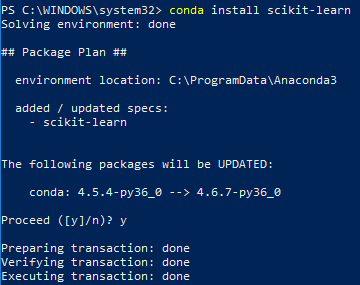
\includegraphics[scale=0.6]{figures/1.png}
\caption{Install Scikit-Learn Conda}
\label{Proses Instalasi}
\end{figure}
\begin{itemize}
\item Lalu ketik "pip install -U scikit-learn" untuk memasukkan anaconda ke python
\end{itemize}
\begin{figure}[ht]
\centering
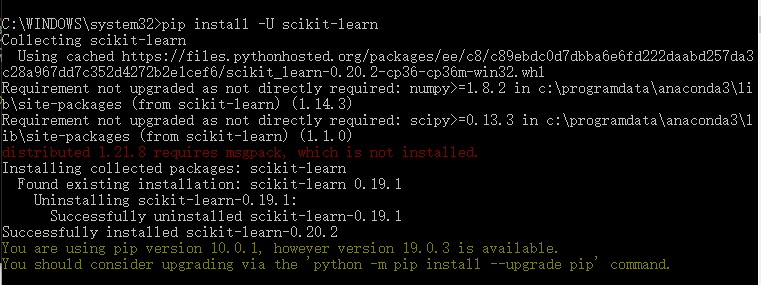
\includegraphics[scale=0.5]{figures/2.png}
\caption{Install Scikit-Learn ke Python}
\label{Gabung Conda dan Python}
\end{figure}
\begin{itemize}
\item Setelah itu, kompilasi kode di dalam python dengan ketik "python", lalu "print('Zulfikar')" maka akan menghasilkan seperti gambar berikut.
\end{itemize}
\begin{figure}[ht]
\centering
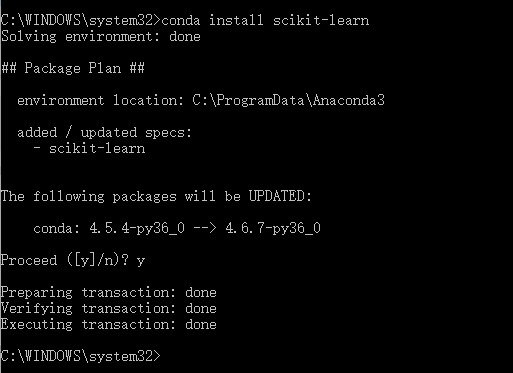
\includegraphics[scale=0.6 ]{figures/3.png}
\caption{Kompilasi Kode}
\label{Kompilasi Kode}
\end{figure}
\item Loading an Example Dataset
\begin{itemize}
\item Ketik perintah berikut "from sklearn import datasets" untuk mengimport dataset dari sklearn.
\end{itemize}
\begin{figure}[ht]
\centering
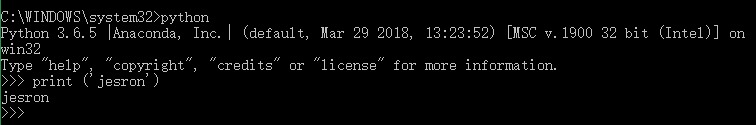
\includegraphics[scale=0.5]{figures/4.png}
\caption{Import Datasets}
\label{Import Datasets}
\end{figure}
\begin{itemize}
\item Kemudian ketik perintah berikut  untuk membuat variable iris yang berisi datasets.
\end{itemize}
\begin{figure}[ht]
\centering
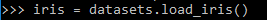
\includegraphics[scale=0.9]{figures/5.png}
\caption{Buat variable iris}
\label{Variable Iris}
\end{figure}
\begin{itemize}
\item Lalu ketik perintah berikut untuk membuat variable digits yang berisi datasets, dan juga untuk melihat isi data dari datasets seperti gambar 1.6 .
\end{itemize}
\begin{figure}[ht]
\centering
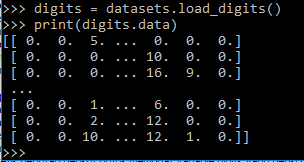
\includegraphics[scale=0.7]{figures/8.png}
\caption{Buat variable digits}
\label{Variable Digits}
\end{figure}
\end{enumerate}

\section{Jesron Marudut Hatuan/1164077}
\subsection{Teori}
\begin{enumerate}
\item Definisi, sejarah, dan perkembangan kecerdasan buatan.
\subitem Kecerdasan Buatan (Artificial Intelligence atau AI) dapat didefinisikan sebagai kecerdasan yang ditunjukkan oleh suatu entitas buatan. Sistem seperti ini biasanya dianggap komputer. Kecerdasan diciptakan lalu dimasukkan ke dalam suatu mesin atau komputer supaya dapat melakukan pekerjaan-pekerjan yang dapat dilakukan manusia.
\subitem Sebenarnya area Kecerdasan Buatan (Artificial Intelligence) atau disingkat dengan AI, dimulai dari munculanya komputer sekitar tahun 1940-an, meskipun sejarah perkembangannya dapat dilacak dari zaman Mesir kuno. Pada akhir tahun 1955, Newell dan Simon mengembangkan The Logic Theorist atau program AI terdahulu. Program ini merepresentasikan masalah sebagai model pohon, lalu penyelesaiannya dengan  memilih cabang yang akan menghasilkan kesimpulan terbenar. Program tersebut berdampak besar dan menjadi batu loncatan dalam mengembangkan bidang AI. Pada tahun 1956 John McCarthy dari  Massacuhetts Institute of Technology dianggap sebagai bapak AI, menyelenggarakan konferensi untuk menarik para ahli komputer bertemu, dengan  nama kegiatan The Dartmouth Summer Research Project On AI. Konferensi Dartmouth saat itu mempertemukan para pendiri dalam AI, dan bertugas untuk meletakkan dasar bagi masa depan  pemgembangan dan penelitian AI. John McCarthy  disaat itu mengusulkan definisi AI adalah AI merupakan cabang dari ilmu komputer yang berfokus pada pengembangan komputer agar mempunyai kemampuan dan berprilaku seperti manusia.
\item  Definisi supervised learning, klasifikasi, regresi, dan unsupervised learning. Data set, training set dan testing set. 
\subitem Supervised learning merupakan sebuah pendekatan dimana sudah terdapat data yang dilatih, dan terdapat variable yang ditargetkan sehingga tujuan dari pendekatan ini adalah mengkelompokan suatu data ke data yang sudah ada. Sedangkan unsupervised learning tidak memiliki data latih, sehingga dari data yang ada, kita mengelompokan data tersebut menjadi 2 bagian atau 3 bagian dan seterusnya.
\subitem Klasifikasi adalah salah satu topik utama dalam data mining atau machine learning. Klasifikasi yaitu suatu pengelompokan data dimana data yang digunakan tersebut mempunyai kelas label atau target.
\subitem Regresi adalah Supervised learning tidak hanya mempelajari classifier, tetapi juga mempelajari fungsi yang dapat memprediksi suatu nilai numerik. Contoh, ketika diberi foto seseorang, kita ingin memprediksi umur, tinggi, dan berat orang yang ada pada foto tersebut.
\subitem Data set adalah cabang aplikasi dari Artificial Intelligence/Kecerdasan Buatan yang fokus pada pengembangan sebuah sistem yang mampu belajar sendiri tanpa harus berulang kali di program oleh manusia.
\subitem Training set yaitu jika pasangan objek, dan kelas yang menunjuk pada objek tersebut adalah suatu contoh yang telah diberi label akan menghasilkan suatu algoritma pembelajaran.
\subitem Testing set digunakan untuk mengukur sejauh mana classifier berhasil melakukan klasifikasi dengan benar\cite{zhu2009introduction}.
\end{enumerate}


\subsection{Instalasi}
\subsubsection{Instalasi Library Scikit dari Anaconda}
\begin{enumerate}
\item Sediakan aplikasi Anaconda terlebih dahulu
\begin{figure}[ht]
\centerline{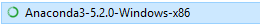
\includegraphics[width=1\textwidth]{figures/0.PNG}}
\caption{Applikasi Anaconda.}
\end{figure}
\item Setelah di install, masukkan script dibawah ini untuk melihat versi Python dan Anacondanya
\begin{figure}[ht]
\centerline{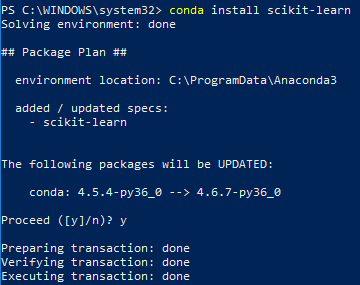
\includegraphics[width=0.75\textwidth]{figures/1.JPEG}}
\caption{Versi Anaconda.}
\end{figure}
\item  Selanjutnya masukkan perintah 'pip install -U scikit-learn'
\begin{figure}[ht]
\centerline{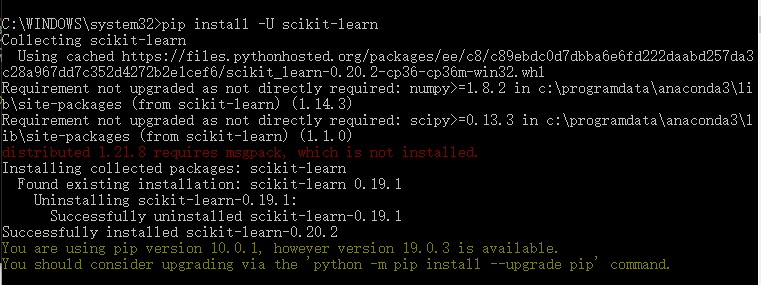
\includegraphics[width=0.75\textwidth]{figures/2.JPEG}}
\caption{Instalasi.}
\end{figure}
\item  Selanjutnya masukkan perintah 'conda install  scikit-learn'
\begin{figure}[ht]
\centerline{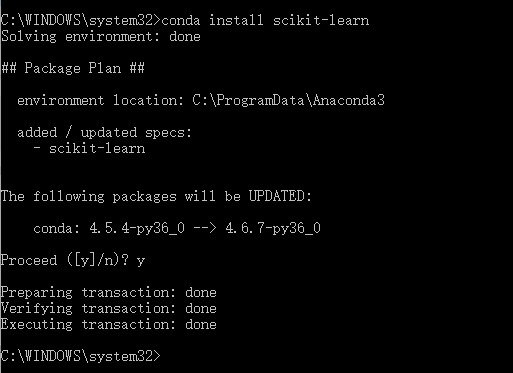
\includegraphics[width=0.75\textwidth]{figures/3.JPEG}}
\caption{Langkah installasi anaconda.}
\end{figure}
\item  Selanjutnya masukkan perintah 'python' dan 'print ('jesron')
\begin{figure}[ht]
\centerline{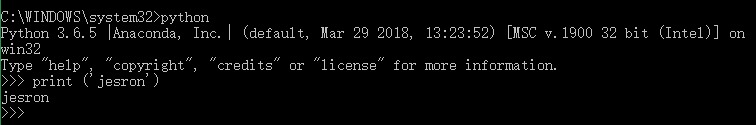
\includegraphics[width=0.5\textwidth]{figures/4.JPEG}}
\caption{Langkah terakhir.}
\end{figure}
\end{enumerate}

<<<<<<< HEAD


=======
\section{Teori/Puad Hamdani/1164084}
\begin{enumerate}
\item Definisi, Sejarah dan Perkembangan Kecerdasan Buatan
\begin{itemize}
\item Definisi
\par
Kecerdasan buatan adalah ilmu pengetahuan yang berhubungan dengan mesin untuk memecahkan persoalan rumit dengan cara yang mudah,dilakukan dengan mengikuti kecerdasan manusia dan menerapkanya di computer sebagai algoritma
\par
\item Sejarah dan Perkembangan
\par
AI (artificial Intelligence) di kenal sekitar tahun 1943 Teori tentang jaringan saraf tiruan (artificial neuron network, ANN) menyatakan bahwa setiap neuron dapat dimisalkan dalam keadaan biner, yaitu ON dan OFF. Dari setiap percobaan, setiap fungsi perhitungan dapat diselesaikan melalui jaringan neuron yang dimodelkan.
Pada tahun 1965, Lotfi Zadeh, professor teknik elektro di University of California, memublikasikan konsepnya yang disebut dengan “fuzzy sets”. Beliau menjabarkan FL dengan pernyataan matematis dan visual yang mudah dipahami. Karena kajian ini berkaitan dengan sistem kontrol, konsep tersebut banyak dikembangkan dalam konteks pemrograman komputer hingga saat ini.
\end{itemize}
\item Definisi Supervised Learning, Unsupervised Learning, Klasifikasi, Regresi, Data Set, Training Set dan Testing Set
\begin{itemize}
\item Supervised Learning 
\par
Supervised learning adalah pembelajaran yang terawasi dimana jika output yang diharapkan telah diketahui sebelumnya. Biasanya pembelajaran ini dilakukan dengan menggunakan data yang telah ada
\item Unsupervised Learning
\par
Unsupervised learning adalah pembelajaran yang tidak terawasi dimana tidak memerlukan target output. Metode ini tidak dapat ditentukan hasil seperti apa yang diharapkan selama proses pembelajaran, Nilai bobot yang disusun dalam proses range tertentu tergantung pada output yang diberikan.
\item Klasifikasi
\par
Klasifikasi adalah Proses pengelompokkan berdasarkan ciri-ciri persamaan dan perbedaan
\item Regresi
\par
Regresi adalah metode analisis statistik yang digunakan untuk melihat pengaruh antara dua atau lebih variabel
\item Data Set
\par
Data set adalah objek yang merepresentasikan data dan relasinya di memory, Strukturnya hampir mirip dengan data di data base. Data set berisi koleksi dari data table dan data relation 
\item Training Set
\par
Training set adalah bagian dataset yang kita latih untuk membuat prediksi atau algoritma ML lainnya sesuai tujuannya masing-masing. Kita memberikan petunjuk melalui algoritma agar mesin yang kita latih bisa mencari korelasinya sendiri. Walau demikian proses belajar harusnya proporsional. Layaknya seorang murid yang terlalu diforsir belajar, maka hasilnya pun tidak akan baik. Dalam istilah ML disebut dengan overfitting. Akan lebih mudah memahami konsep overfitting melalui praktek.
\item Testing Set
\end{itemize}
\par
Test set adalah bagian dataset yang kita tes untuk melihat keakuratannya, atau dengan kata lain melihat performanya.
\item Instalasi Scikit-Learn dari Anaconda
\begin{itemize}
\item Pertama install Anaconda di pc masing-masing
\item Kemudian buka cmd untuk menginstall scikit-learn
\item Ketikan "conda install scikit-learn" dan pilih "y"
\end{itemize}
\begin{figure}[ht]
\centering
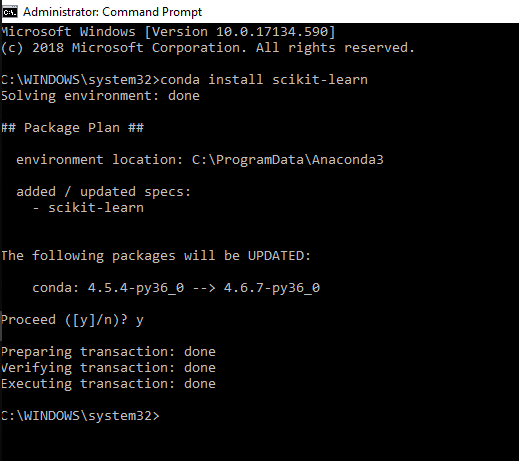
\includegraphics[scale=0.6]{figures/puad1.png}
\caption{Proses Instalasi}
\end{figure}
\begin{itemize}
\item ketik "pip install -U scikit-learn" untuk menggabungkan anaconda dan python
\end{itemize}
\begin{figure}[ht]
\centering
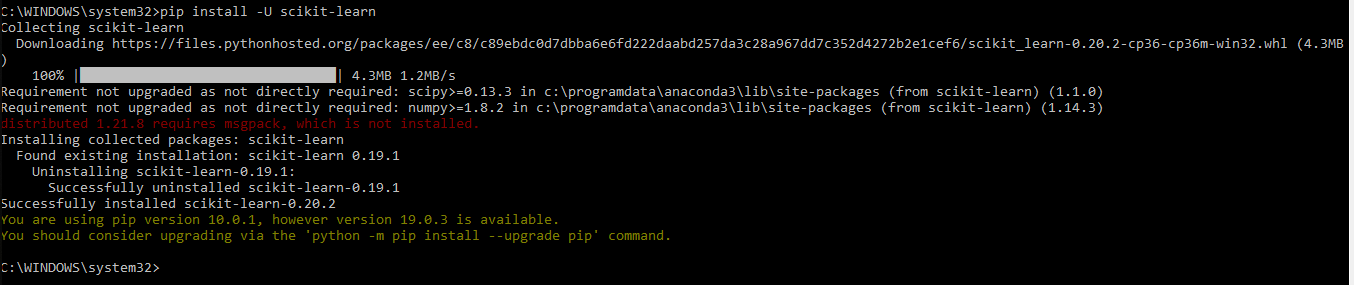
\includegraphics[scale=0.5]{figures/puad2.png}
\caption{Gabung Conda dan Python}
\end{figure}
\begin{itemize}
\item Setelah itu, kompilasi kode di dalam python dengan ketik "python", lalu "print('puad')" maka akan menghasilkan seperti gambar berikut.
\end{itemize}
\begin{figure}[ht]
\centering
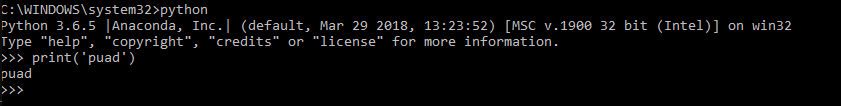
\includegraphics[scale=0.6 ]{figures/puad3.png}
\caption{Kompilasi Kode}
\end{figure}
\item Loading an Example Dataset
\begin{itemize}
\item Ketik perintah berikut "from sklearn import datasets" untuk mengimport dataset dari sklearn.
\end{itemize}
\begin{itemize}
\item ketik perintah "iris = datasets.load iris" untuk membuat variable iris yang berisi datasets.
\end{itemize}
\begin{itemize}
\item ketik perintah berikut"digits = datasets.load digits"untuk membuat variable digits yang berisi datasets, dan juga "print(digits.data) " untuk melihat isi data dari datasets seperti gambar 
\end{itemize}
\begin{figure}[ht]
\centering
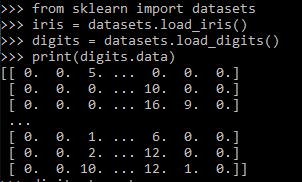
\includegraphics[scale=0.7]{figures/puad4.png}
\caption{Variable Digits}
\end{figure}
\begin{itemize}
\item kemudian  ketik "digits target"
\end{itemize}
\begin{figure}[ht]
\centering
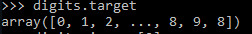
\includegraphics[scale=0.5]{figures/puad5.png}
\caption{}
\end{figure}
\begin{itemize}
\item kemudian  ketik "digits.images[0] "
\end{itemize}
\begin{figure}[ht]
\centering
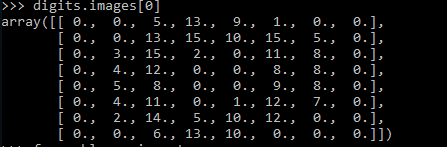
\includegraphics[scale=0.5]{figures/puad6.png}
\caption{}
\end{figure}
\begin{itemize}
\item kemudian  ketik "from sklearn import svm" dan kemudian clf = svm.SVC(gamma=0.001, C=100.) "
\item kemudian  ketik "clf.fit(digits.data[:-1], digits.target[:-1]) "
\end{itemize}
\begin{figure}[ht]
\centering
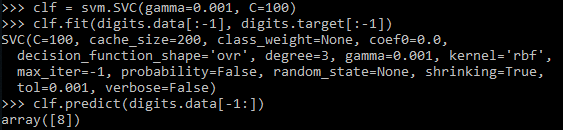
\includegraphics[scale=0.5]{figures/puad7.png}
\caption{}
\end{figure}
\begin{itemize}
\item kemudian  ketik "clf.predict(digits.data[-1:])"
\end{itemize}
\begin{figure}[ht]
\centering
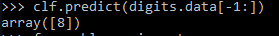
\includegraphics[scale=0.5]{figures/puad8.png}
\caption{}
\end{figure}
\begin{itemize}
\item kemudian  ketik "from sklearn import svm"
\item kemudian  ketik "from sklearn import datasets"
\item kemudian  ketik "clf = svm.SVC(gamma='scale')"
\item kemudian  ketik "iris = datasets.load(andeskore)iris()"
\item kemudian  ketik "X, y = iris.data, iris.target"
\item kemudian  ketik "clf.fit(X, y) "
\end{itemize}
\begin{figure}[ht]
\centering
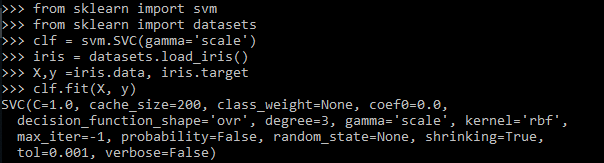
\includegraphics[scale=0.5]{figures/puad9.png}
\caption{}
\end{figure}
\begin{itemize}
\item kemudian  ketik "import pickle"
\item kemudian  ketik "s = pickle.dumps(clf)"
\item kemudian  ketik "clf2 = pickle.loads(s)"
\item kemudian  ketik "clf2.predict(X[0:1])"
\end{itemize}
\begin{figure}[ht]
\centering
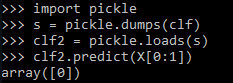
\includegraphics[scale=0.5]{figures/puad10.png}
\caption{}
\end{figure}
\begin{itemize}
\item kemudian  ketik " y[0]"
\end{itemize}
\begin{figure}[ht]
\centering
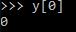
\includegraphics[scale=0.5]{figures/puad11.png}
\caption{}
\end{figure}
\begin{itemize}
\item kemudian  ketik "from joblib import dump, load"
\item kemudian  ketik "dump(clf, 'filename.joblib')"
\end{itemize}
\begin{figure}[ht]
\centering
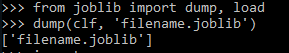
\includegraphics[scale=0.5]{figures/puad13.png}
\caption{}
\end{figure}
\begin{itemize}
\item conventions
\item ketikan "import numpy as np"
\item ketikan "from sklearn import random(andeskor)projection"
\item ketikan "rng = np.random.RandomState(0)"
\item ketikan "X = rng.rand(10, 2000)"
\item ketikan "X = np.array(X, dtype='float32')"
\item ketikan "X.dtype"
\item ketikan "transformer = random projection.GaussianRandomProjection"
\item ketikan "X new = transformer.fit transform(X)"
\item ketikan "X new.dtype"
\end{itemize}
\begin{figure}[ht]
\centering
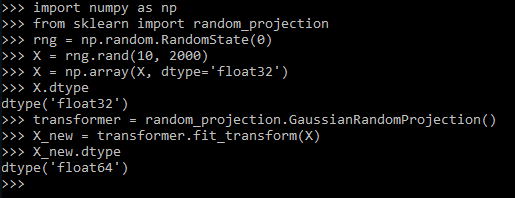
\includegraphics[scale=0.5]{figures/puad14.png}
\caption{}
\end{figure}
\item screenshoot eror
\begin{figure}[ht]
\centering
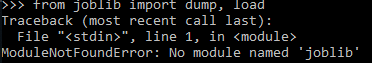
\includegraphics[scale=0.5]{figures/puad12.png}
\caption{}
\end{figure}
\item kode eror "no module named 'joblib'"
\item penanganannya instal joblib dengan mengetikan"conda instal -c anaconda joblib"
\end{enumerate}
>>>>>>> efee6eca5df5ee495d6544dd76ec774eee595c8a
=======
<<<<<<< HEAD
\section{Instalasi/Mhd Zulfikar Akram Nasution/1164081}
\begin{enumerate}
\item Menjelaskan Kode dari Learning and Predicting
\begin{itemize}
\item Pertama import file smv dari sklearn seperti pada gambar 1.12
\end{itemize}
\begin{figure}[ht]
\centering
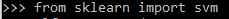
\includegraphics[scale=0.9]{figures/2_1.png}
\caption{Import file svm}
\label{Import svm}
\end{figure}
\begin{itemize}
\item Kemudian buat variabel clf seperti pada gambar 1.13
\end{itemize}
\begin{figure}[ht]
\centering
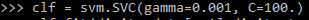
\includegraphics[scale=0.9]{figures/2_2.png}
\caption{Buat variable Classifier}
\label{Variabel clf}
\end{figure}
\begin{itemize}
\item Lalu ketik kode berikut untuk meliat array baru dari syntax python [:-1] sepert padai gambar 1.14
\end{itemize}
\begin{figure}[ht]
\centering
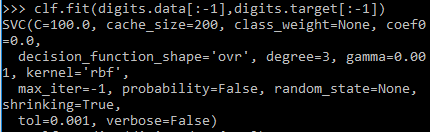
\includegraphics[scale=0.7]{figures/2_3.png}
\caption{Lihat array baru dengan syntac Python}
\label{Syntax python}
\end{figure}
\begin{itemize}
\item Selanjutnya ketikkan kode berikut untuk melihat penggolongan array seperti pada gambar 1.15
\end{itemize}
\begin{figure}[ht]
\centering
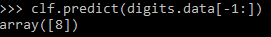
\includegraphics[scale=0.7]{figures/2_4.png}
\caption{Lihat classifier array}
\label{Classifier Array}
\end{figure}
\item Model Persistence
\begin{itemize}
\item Pertama Import dulu file dari sklearn
\end{itemize}
\begin{figure}[ht]
\centering
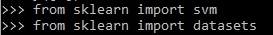
\includegraphics[scale=0.7]{figures/2_5.png}
\caption{Import file}
\end{figure}
\begin{itemize}
\item Kemudian buat variable classifier dengan gamma=scale
\end{itemize}
\begin{figure}[ht]
\centering
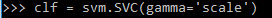
\includegraphics[scale=0.9]{figures/2_6.png}
\caption{Variable classifier}
\end{figure}
\begin{itemize}
\item Lalu buat variable iris dan (X,y)
\end{itemize}
\begin{figure}[ht]
\centering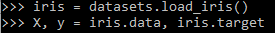
\includegraphics[scale=0.9]{figures/2_7.png}
\caption{Variable iris}
\end{figure}
\begin{itemize}
\item Selanjutnya kita akan melihat penyesuaian classifier
\end{itemize}
\begin{figure}[ht]
\centering
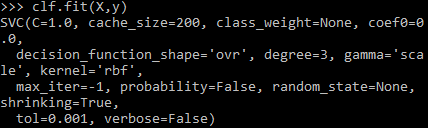
\includegraphics[scale=0.7]{figures/2_8.png}
\caption{Penyesuaian Classifier}
\end{figure}
\begin{itemize}
\item Kemudian import pickle untuk melihat hasil array dan hasil y
\end{itemize}
\begin{figure}[ht]
\centering
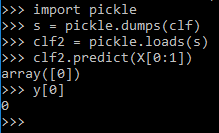
\includegraphics[scale=0.7]{figures/2_9.png}
\caption{Import Pickle}
\end{figure}
\item Conventions
\begin{itemize}
\item Pertama import numpy menjadi np serta import random projection
\end{itemize}
\begin{figure}[ht]
\centering
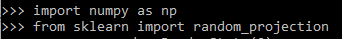
\includegraphics[scale=0.7]{figures/2_10.png}
\caption{Import numpy}
\end{figure}
\begin{itemize}
\item Kemudian buat variable rng dengan type random
\end{itemize}
\begin{figure}[ht]
\centering
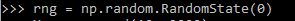
\includegraphics[scale=0.7]{figures/2_11.png}
\caption{Variable rng}
\end{figure}
\begin{itemize}
\item Lalu buat variable X, dan lihat hasil rng random yang keluar
\end{itemize}
\begin{figure}[ht]
\centering
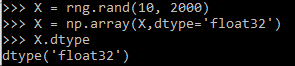
\includegraphics[scale=0.9]{figures/2_12.png}
\caption{Variable X dan hasil random}
\end{figure}
\begin{itemize}
\item Setelah itu buat variable transformer dengan type random
\end{itemize}
\begin{figure}[ht]
\centering
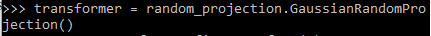
\includegraphics[scale=0.9]{figures/2_13.png}
\caption{Variable transformer random}
\end{figure}
\begin{itemize}
\item Berikutnya itu buat variable X new dengan type yang ada pada tranformer
\end{itemize}
\begin{figure}[ht]
\centering
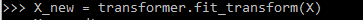
\includegraphics[scale=0.9]{figures/2_14.png}
\caption{Variable X new type pada transformer}
\end{figure}
\begin{itemize}
\item Kemudian lihat hasil dari X new
\end{itemize}
\begin{figure}[ht]
\centering
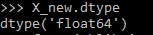
\includegraphics[scale=0.9]{figures/2_15.png}
\caption{Hasil dari X new type pada transformer}
\end{figure}
\item Screenshoot Error pada gambar 1.27
\begin{figure}[ht]
\centering
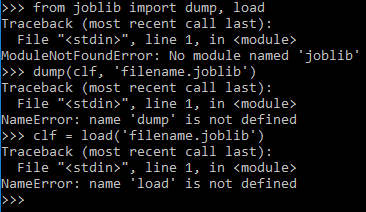
\includegraphics[scale=0.7]{figures/2_16.png}
\caption{Screenshoot Error}
\end{figure}
\item Kode yang error yaitu "joblib" karena belum ada library nya seperti pada gambar 1.28
\item Solusi dari masalah yang error seperti pada gambar 1.29
\begin{figure}[ht]
\centering
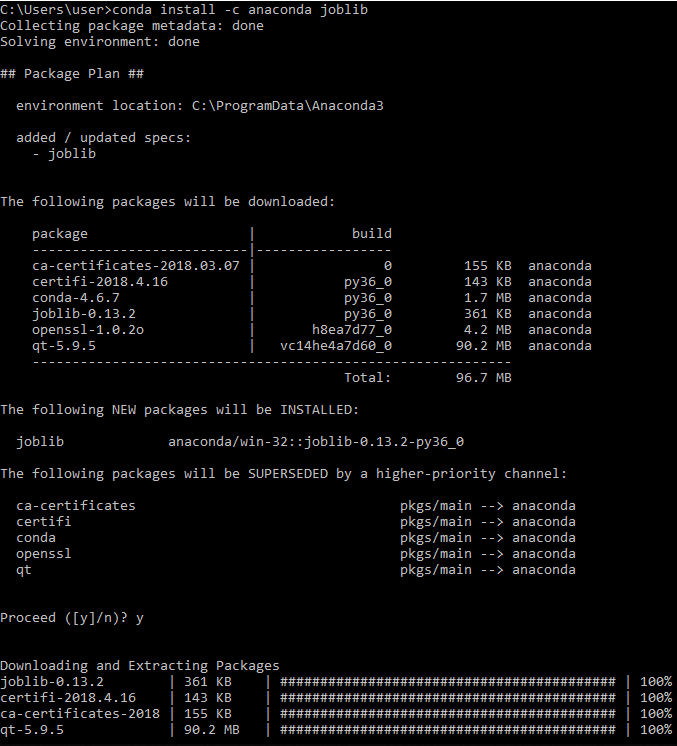
\includegraphics[scale=0.3]{figures/2_17.png}
\caption{Install Joblib}
\end{figure}
\begin{figure}[ht]
\centering
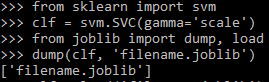
\includegraphics[scale=0.7]{figures/2_18.png}
\caption{Solusi Error}
\end{figure}


\end{enumerate}
=======
\subsection{Installasi}
\subsubsection{Loading an Example Datasets}
\begin{enumerate}
\item Loading an Example Dataset
\begin{itemize}
\item Ketik perintah berikut "from sklearn import datasets" untuk mengimport dataset dari file sklearn tadi.
\end{itemize}
\begin{figure}[ht]
\centering
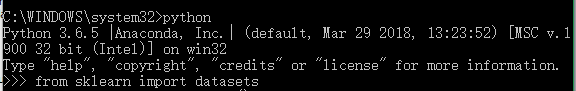
\includegraphics[scale=0.5]{figures/satu.png}
\caption{Perintah sklearn import datasets}
\label{Import Datasets}
\end{figure}
\begin{itemize}
\item Selanjutnya ketik perintah berikut ini untuk membuat variable iris yang berisi datasets.
\end{itemize}
\begin{figure}[ht]
\centering
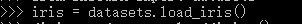
\includegraphics[scale=0.9]{figures/dua.png}
\caption{Perintah Variabel Iris}
\label{Variable Iris}
\end{figure}
\begin{itemize}
\item Masukkan perintah ini untuk membuat variable digits yang berisi datasets, dapat juga untuk melihat isi data dari datasets tadi.
\end{itemize}
\begin{figure}[ht]
\centering
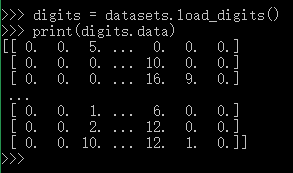
\includegraphics[scale=0.9]{figures/tiga.png}
\caption{Perintah Variabel Digits}
\label{Variable Digits}
\end{figure}
\end{enumerate}


\section{Learning and Predicting}
\begin{itemize}
\item from sklearn import svm ( pada baris berikut ini merupakan sebuah perintah untuk mengimport class svm dari package sklearn).
\item clf = svm.SVC (gamma=0.001, C=100.) (pada baris kedua ini clf sebagai estimator atau parameter, svm.SVC menjadi sebuah class, dan gamma sebagai parameter untuk menetapkan nilai secara manual)
\item clf.fit(digits.data[:-1], digits.target[:-1]) (pada baris ketiga ini clf sebagai estimator atau parameter, fit sebagai metode, digits.data sebagai item, [:-1] sebagai syntax pythonnya dan menampilkan outputannya)
\item clf.predict(digits.data[-1:])
\end{itemize}
\subsubsection{Model Presistence}
\begin{itemize}
\item from sklearn import svm
\item from sklearn import datasets
\item clf = svm.SVC(gamma='scale')
\item iris = datasets.load\_iris()
\item X, y = iris.data, iris.target
\item clf.fit(X, y)hasil
\item import pickle
\item s = pickle.dumps(clf)
\item clf2 = pickle.loads(s)
\item clf2.predict(X[0:1])hasil
\item y[0]hasil
\item from joblib import dump, load eror
\item dump(clf, 'filename.joblib')eror
\item clf = load('filename.joblib')eror
\end{itemize}
\subsubsection{Conventions}
\begin{enumerate}
\item Type Casting
\begin{itemize}
\item from sklearn import svm
\item from sklearn import random\_projection
\item rng = np.random.RandomState(0)
\item X = rng.rand(10, 2000)
\item X = np.array(X, dtype='float32')
\item X.dtype hasil
\item transformer = random\_projection.GaussianRandomProjection()
\item X\_new = transformer.fit\_transform(X)
\item X\_new.dtype hasil
\item from sklearn import datasets
\item from sklearn.svm import SVC
\item iris = datasets.load\_iris()
\item clf = SVC(gamma='scale')
\item clf.fit(iris.data, iris.target)hasil
\item list(clf.predict(iris.data[:3])) hasil
\item clf.fit(iris.data, iris.target\_names[iris.target]) hasil
\item list(clf.predict(iris.data[:3])) hasil
\end{itemize}
\item Refitting and Updating Parameters
\begin{itemize}
\item import numpy as np
\item from sklearn.svm import SVC
\item rng = np.random.RandomState(0)
\item X = rng.rand(100, 10)
\item y = rng.binomial(1, 0.5, 100)
\item X\_test = rng.rand(5, 10)
\item clf = SVC()
\item clf.set\_params(kernel='linear').fit(X, y) hasil
\item clf.predict(X\_test) hasil
\item clf.set\_params(kernel='rbf', gamma='scale').fit(X, y) hasil
\item clf.predict(X\_test) hasil
\end{itemize}
\item Multiclass vs. Multilabel Fitting
\begin{itemize}
\item from sklearn.svm import SVC
\item from sklearn.multiclass import OneVsRestClassifier
\item from sklearn.preprocessing import LabelBinarizer
\item X = [[1, 2], [2, 4], [4, 5], [3, 2], [3, 1]]
\item y = [0, 0, 1, 1, 2]
\item classif = OneVsRestClassifier(estimator=SVC(gamma='scale',random\_state=0))
\item classif.fit(X, y).predict(X) hasil
\item y = LabelBinarizer().fit\_transform(y)
\item classif.fit(X, y).predict(X) hasil
\item from sklearn.preprocessing import MultiLabelBinarizer
\item y = [[0, 1], [0, 2], [1, 3], [0, 2, 3], [2, 4]]
\item y = MultiLabelBinarizer().fit\_transform(y)
\item classif.fit(X, y).predict(X) hasil
\end{itemize}
\end{enumerate}

\section{Penanganan Error}
\begin{enumerate}
\item
Dibawah ini merupakan error yang ditemukan pada saat melakukan percobaan import.
\begin{figure}
\begin{center}
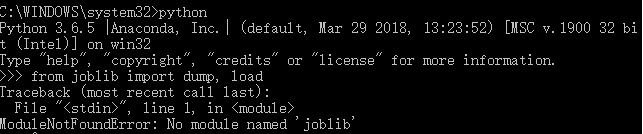
\includegraphics[scale=0.75]{figures/Error1.png}
\caption{Error Import}
\end{center}
\end{figure}
\item
Pada gambar diatas, terjadi error ketika sedang mengimport modul yang telah ditetapkan.
\item
Solusinya dapat dilakukan dengan berikut ini :\\
Error tadi terjadi akibat Library Joblib pada PC belum terinstall. Oleh sebab itu, install terlebih dahulu.
\item
Dengan membuka CMD (Admin), kemudian masukkan perintah "pip install joblib" dan tunggu sampai installasi berhasil seperti gambar berikut.
\begin{figure}
\begin{center}
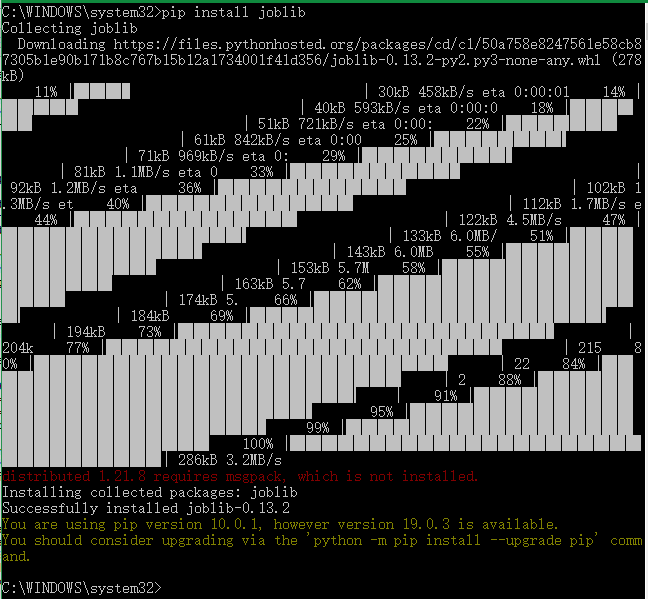
\includegraphics[scale=0.5]{figures/install2.png}
\caption{Install Library Joblib}
\end{center}
\end{figure}
\item
Ketika sudah terinstall, maka bisa dilakukan lagi import library joblib, dan hasilnya akan tampil seperti dibawah ini
\begin{figure}
\begin{center}
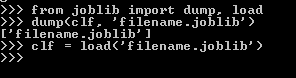
\includegraphics[scale=1]{figures/hasil3.png}
\caption{Berhasil Import Library Joblib}
\end{center}
\end{figure}
\end{enumerate}




>>>>>>> 
>>>>>>> f594df5d4cf2e0a7297e57a9c544d6f3fac837ab
>>>>>>> 2951ffb45da2a049bd0331edf27d34ed0e23f9f5

\chapter{Related Works}

Your related works, and your purpose and contribution which must be different as below.

<<<<<<< HEAD
\section{Mhd Zulfikar Akram Nasution/ 1164081}
\subsection{Teori}
\begin{enumerate}
\item Binary Classification atau diartikan kedalam bahasa indonesia yaitu Klasifikasi Biner adalah tugas dalam mengklarifikasikan elemen-elemen dari himpunan yang diberikan kedalam dua kelompok berdasarkan aturan klarifikasi. Pada ummnya klarifikasi biner akan jatuh ke dalam domain Supervised Learning dan dimana kasus khusus hanya memiliki dua kelas.
\begin{itemize}
\item  Contoh Binary Classification pada gambar 2.1
\end{itemize}
\begin{figure}[ht]
\centering
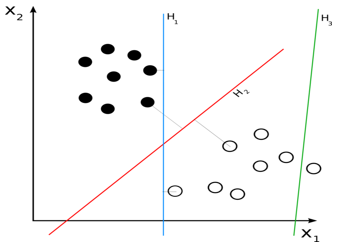
\includegraphics[scale=0.9]{figures/zulfikar/1.png}
\caption{Binary Classification}
\end{figure}

\item Supervised Learning, Unsupervised Learning, dan Clustering
\begin{itemize}
\item Supervised Learning
\end{itemize}
\par
Supervised learning adalah tugas pembelajaran mesin untuk mempelajari suatu fungsi yang memetakan input ke output berdasarkan contoh pasangan input-output. Ini menyimpulkan fungsi dari data pelatihan berlabel yang terdiri dari serangkaian contoh pelatihan. Dalam pembelajaran yang diawasi, setiap contoh adalah pasangan yang terdiri dari objek input (biasanya vektor) dan nilai output yang diinginkan (juga disebut sinyal pengawas). Contoh pada gambar 2.2
\begin{figure}[ht]
\centering
\includegraphics[scale=0.9]{figures/zulfikar/2.png}
\caption{Supervised Learning}
\end{figure}

\begin{itemize}
\item Unsupervised Learning
\end{itemize}
\par
Unsupervised Learning merupakan sebuah data yang belum ditentukan variabelnya jadi hanya berupa data saja. Dalam sebuah kasus Unsupervised Learning adalah aggap saja anda belum pernah membeli buku sama sekali dan pada suatu hari anda telah membeli buku dengan sangat banyak dalam kategori yang berbeda. Sehingga buku tersebut belum di kategorikan dan hanya berupa data buku saja. Coontoh seperti pada gambar 2.3
\begin{figure}[ht]
\centering
\includegraphics[scale=0.9]{figures/zulfikar/3.png}
\caption{Unsupervised Learning}
\end{figure}

\begin{itemize}
\item Clustering
\end{itemize}
\par
 Classtering merupakan sebuah proses untuk mengklasifikasikan sebuah data dalam satu parameter. Dalam kasus ini dapat dijelaskan ada beberapa orang yang memiliki kekuatan tubuh yang sehat dan kekuatan tubuh yang lemah. Parameter bagi orang yang memiliki tubuh yang kuat adalah orang yang terlihat bugar dan sehat maka dengan orang yang memiliki parameter adalah orang yang memiliki kekuatan tubuh yang kuat dan untuk kekuatan tubuh yang lemah adalah sebaliknya. Contoh seperti pada gambar 2.4
\begin{figure}[ht]
\centering
\includegraphics[scale=0.9]{figures/zulfikar/4.png}
\caption{Clustering}
\end{figure}

\item Evaluasi dan Akurasi
\par
 Evaluasi adalah tentang  bagaimana kita dapat mengevaluasi seberapa baik model bekerja dengan mengukur akurasinya. Dan akurasi akan didefinisikan sebagai persentase kasus yang diklasifikasikan dengan benar. Kita dapat menganalisis kesalahan yang dibuat oleh model, atau tingkat kebingungannya, menggunakan matriks kebingungan. Matriks kebingungan mengacu pada kebingungan dalam model, tetapi matriks kebingungan ini bisa menjadi sedikit sulit untuk dipahami ketika mereka menjadi sangat besar.

\item Cara Membuat dan Membaca Confusion Matrix
\begin{itemize}
\item Tentukan pokok permasalahan dan atributnya
\item Buat Decicion Tree
\item Buat Data Testing
\item Mencari nilai variabelnya misal a,b,c, dan d
\item Mencari nilai recall, percision, accuracy, dan error rate
\end{itemize}
\par contoh confusion matrix
	\begin{verbatim}
		Recall = 3/(1+3) = 0,75
		Percision = 3/(1+3 = 0,75
		Accuracy = (5+3)/(5+1+1+3) = 0,8
		Error Rate = (1+1)/(5+1+1+3) 0,2
	\end{verbatim}

\item Cara Kerja K-Fold Cross Validation
	\begin{itemize}
		\item Total instance dibagi menjadi N bagian.
		\item Fold yang pertama adalah bagian pertama menjadii testing data dan sisanya menjadi training data.
		\item Hitung akurasi berdasarkan porsi data tersebut dengan menggunakan persamaan.
		\item Fold yang ke dua adalah bagian ke dua menjadi testing data dan sisanya training data. 
		\item Hitung akurasi berdasarkan porsi data tersebut.
		\item Lakukan step secara berulang hingga habis mencapai fold ke-K.
		\item Terakhir hitung rata-rata akurasi K buah.
	\end{itemize}
\par
Berikut ilustrasi K-Fold Cross Validation seperti pada gambar 2.5
\begin{figure}[ht]
\centering
\includegraphics[scale=0.9]{figures/zulfikar/5.png}
\caption{K-Fold Cross Validation}
\end{figure}

\item Decision Tree
\par 
Decision Tree adalah sebuah metode pembelajaran yang digunakan untuk melakukan klarifikasi dan regresi. Decision Tree digunakan untuk membuat sebuah model yang dapat memprediksi sebuah nilai variabel target dengan cara mempelajari aturan keputusan dari fitur data. Contohnya seperti pada gambar 2.6 
\begin{figure}[ht]
\centering
\includegraphics[scale=0.9]{figures/zulfikar/6.png}
\caption{Decision Tree}
\end{figure}

\item Gain dan Entropi
\begin{itemize}
\item Gain adalah pengurangan yang diharapkan dalam enthropy. Dalam mechine learning, gain dapat digunakan untuk menentukan sebuah urutan atribut atau memperkecil atribut yang telah dipilih. Urutan ini akan membentuk decision tree. atribut gain dipilih yang paling besar.
\item  Entropi adalah ukuran ketidakpastian sebuah variabel acak sehingga dapat di artikan entropi adalah ukuran ketidakpastian dari sebuah atribut.
\end{itemize}
\par Contoh seperti pada gambar 2.7
\begin{figure}[ht]
\centering
\includegraphics[scale=0.9]{figures/zulfikar/7.png}
\caption{Gain dan Entropi}
\end{figure}
\end{enumerate}

\section{Mhd Zulfikar Akram Nasution/ 1164081}
=======

\section{puad hamdani/1164084}
\subsection{binary classification }
\begin{enumerate}
\item Output aktual dari banyak algoritma binary classification adalah skor prediksi. Skor menunjukkan kepastian sistem bahwa pengamatan yang diberikan adalah milik kelas positif. Untuk membuat keputusan tentang apakah pengamatan harus diklasifikasikan sebagai positif atau negatif
\end{enumerate}

\subsection{supervised learning dan unsupervised learning}
\begin{enumerate}
\item Supervised learning adalah sebuah pendekatan dimana sudah terdapat data yang dilatih, dan terdapat variable yang di targetkan sehingga tujuan dari pendekatan ini adalah mengelompokkan suatu data ke data yang sudah ada.


\item Unsupervised learning adalah istilah yang digunakan untuk pembelajaran bahasa Ibrani, yang terkait dengan pembelajaran tanpa guru, juga dikenal sebagai organisasi mandiri dan metode pemodelan kepadatan probabilitas input. Unsupervised learning tidak memiliki data latih, sehingga dari data yang ada, kita mengelompokan data tersebut menjadi dua bagian atau tiga bagian dan seterusnya.
\end{enumerate}

\subsection{evaluasi dan akurasi }
\begin{enumerate}
\item Evaluasi merupakan suatu proses identifikasi untuk mengukur atau menilai apakah suatu kegiatan/program yang dilaksanakan sesuai dengan perencanaan atau tujuan yang ingin dicapai.
Akurasi merupakan tingkat kedekatan pengukuran kuantitas terhadap nilai yang sebenarnya. Kepresisian dari suatu sistem pengukuran
\end{enumerate}

\subsection{ bagaimana cara membuat dan membaca confusion matrix, buat confusion matrix }
\begin{enumerate}
\item Cara membuat dan membaca confusion matrix :
\begin{itemize}
\item 1)	Tentukan pokok permasalahan dan atributanya
\item 2)	Buat pohon keputusan
\item 3)	Lalu data testingnya
\item 4)	Lalu mencari nilai a, b, c, dan d. Semisal a = 5, b = 1, c = 1, dan d = 3.
\item 5)	Selanjutnya mencari nilai recall, precision, accuracy, serta dan error rate.
\end{itemize}
\item Berikut adalah contoh dari confusion matrix :
\begin{itemize}
\item Recall =3/(1+3) = 0,75
\item Precision = 3/(1+3) = 0,75
\item Accuracy =(5+3)/(5+1+1+3) = 0,8
\item Error Rate =(1+1)/(5+1+1+3) = 0,2
\end{itemize}
\end{enumerate}

\subsection{bagaimana K-fold cross validation bekerja dengan gambar ilustrasi}
\begin{enumerate}
\item Cara kerja K-fold cross validation :
\begin{itemize}
\item 1)	Total instance dibagi menjadi N bagian.
\item 2)	Fold yang pertama adalah bagian pertama menjadi data uji (testing data) dan sisanya menjadi training data.
\item 3)	Lalu hitung akurasi berdasarkan porsi data tersebut dengan menggunakan persamaan.
\item 4)	Fold yang ke dua adalah bagian ke dua menjadi data uji (testing data) dan sisanya training data. 
\item 5)	Kemudian hitung akurasi berdasarkan porsi data tersebut.
\item 6)	Dan seterusnya hingga habis mencapai fold ke-K.
\item 7)	Terakhir hitung rata-rata akurasi K buah.
\end{itemize}
\end{enumerate}

\subsection{decision tree}
\begin{enumerate}
\item Decision tree merupakan model prediksi menggunakan struktur pohon atau struktur berhirarki.
\end{enumerate}

\subsection{Information Gain}
\begin{enumerate}
\item Information gain. Metode tersebut akan melakukan proses komputasi untuk mendapatkan atribut-atribut yang paling berpengaruh terhadap dataset
\end{enumerate}


\section{Puad Hamdani/ 1164084}
>>>>>>> abaa009ed6a2bf07ff821b0fed9603a84340748c
\subsection{Scikit-Learn}

\begin{enumerate}
\item
\begin{verbatim}
	# load dataset (student mat pakenya)
	import pandas as pd
<<<<<<< HEAD
	lontong    = pd.read_csv('student-mat.csv', sep=';')
	len(lontong)
\end{verbatim}
\begin{figure}[ht]
\centering
\includegraphics[scale=0.9]{figures/lontong/1.png}
\caption{Load Dataset}
\end{figure}
\par
	Codingan pertama ini akan meload ( menampilkan ) data pada file yang ditentukan. Untuk codingan ini file yang dieksekusi ialah " student-mat.csv " . Secara jelasnya, dalam codingan dapat dilihat bahwa variabel lontong didefinisikan untuk pembacaan csv dari " lontong " dimana untuk pemisahnya yaitu separation berupa ; . Setelah itu variabel lontong di "print" dengan perintah menampilkan "len" panjang ataupun jumlah dan hasilnya berupa angka 649 . 
=======
\begin{verbatim}
	sate    = pd.read_ csv('student-mat.csv', sep=';')
	len(sate)
\end{verbatim}
\begin{figure}[ht]
\centering
\includegraphics[scale=0.5]{figures/41.png}
\caption{Load Dataset}
\end{figure}
\par
	Codingan ini akan meload ( menampilkan ) data pada file yang ditentukan. hasilnya berupa angka 649 . 
>>>>>>> abaa009ed6a2bf07ff821b0fed9603a84340748c

\item
\begin{verbatim}
	# generate binary label (pass/fail) based on G1+G2+G3 
	# (test grades, each 0-20 pts); threshold for passing is sum>=30
<<<<<<< HEAD
	lontong['pass'] = lontong.apply(lambda row: 1 if (row['G1']+row['G2']+row['G3']) 
											>= 35 else 0, axis=1)
	lontong = lontong.drop(['G1', 'G2', 'G3'], axis=1)
	lontong.head()
\end{verbatim}
\begin{figure}[ht]
\centering
\includegraphics[scale=0.6]{figures/lontong/2.png}
\caption{Generate Binary Label}
\end{figure}
\par
	Codingan kedua ini secara keseluruhan menampilkan  baris  G1, G2 dan G3 ( berdasarkan kriterianya ) untuk kolom PASS pada variabel lontong. Untuk lebih jelasnya, pada codingan terdapat pendefinisian pembacaan "lambda" ( panjang gelombang ) dari baris G1, G2 dan G3. Apabila row-row tersebut bernilai lebih dari 35 maka akan terdefinisikan angka "1" apabila tidak, maka akan terdefinisikan angka "0" pada kolom PASS ( sesuai permintaan awal ). Selanjutnya variabelnya di "print" sehingga menampilkan keluaran. Tidak lupa terdapat juga jumlah dari baris dan kolom yang terubah sesuai dengan baris yang dieksekusi.


\item
\begin{verbatim}
	# use one-hot encoding on categorical columns
	lontong = pd.get_dummies(lontong, columns=['sex', 'school', 'address', 
=======
	sate['pass'] = sate.apply(lambda row: 1 if (row['G1']+row['G2']+row['G3']) 
											>= 35 else 0, axis=1)
	sate = sate.drop(['G1', 'G2', 'G3'], axis=1)
	sate.head()
\end{verbatim}
\begin{figure}[ht]
\centering
\includegraphics[scale=0.6]{figures/42.png}
\caption{Generate Binary Label}
\end{figure}
\par
	Codingan ini secara keseluruhan menampilkan  baris  G1, G2 dan G3 ( berdasarkan kriterianya ). Untuk lebih jelasnya, pada codingan terdapat pendefinisian pembacaan "lambda" ( panjang gelombang ) dari baris G1, G2 dan G3. Apabila row-row tersebut bernilai lebih dari 35 maka akan terdefinisikan angka "1" apabila tidak, maka akan terdefinisikan angka "0"
\item
\begin{verbatim}
	# use one-hot encoding on categorical columns
	sate = pd.get_dummies(sate, columns=['sex', 'school', 'address', 
>>>>>>> abaa009ed6a2bf07ff821b0fed9603a84340748c
									'famsize', 
									'Pstatus', 'Mjob', 'Fjob', 
	                               'reason', 'guardian', 'schoolsup', 
								   'famsup', 'paid', 'activities',
	                               'nursery', 'higher', 'internet', 
									'romantic'])
<<<<<<< HEAD
	lontong.head()
\end{verbatim}
\begin{figure}[ht]
\centering
\includegraphics[scale=0.6]{figures/lontong/3.png}
\caption{Pemanggilan get dummies dari lontong}
\end{figure}
\par
	Secara keseluruhan, codingan ini mendefinisikan pemanggilan get dummies ke dalam variabel lontong. Di dalam get dummies sendiri akan terdefinisikan variabel lontong dengan kolom-kolom yang akan dieksekusi seperti school, address dll. Kemudian variabel tersebut di definisikan untuk mendapatkan kembalian berupa keluaran dari eksekusi perintah variabel lontong beserta dengan jumlah baris dan kolom data yang dieksekusi.
=======
\begin{verbatim}
	sate.head()
\end{verbatim}
\begin{figure}[ht]
\centering
\includegraphics[scale=0.6]{figures/421.png}
\caption{Pemanggilan get dummies}
\end{figure}
\par
	Secara keseluruhan, codingan ini mendefinisikan pemanggilan get dummies ke dalam variabel sate.
>>>>>>> abaa009ed6a2bf07ff821b0fed9603a84340748c

\item
\begin{verbatim}
	# shuffle rows
<<<<<<< HEAD
	lontong = lontong.sample(frac=1)
	# split training and testing data
	lontong_train = d[:500]
	lontong_test = d[500:]

	lontong_train_att = lontong_train.drop(['pass'], axis=1)
	lontong_train_pass = lontong_train['pass']

	lontong_test_att = lontong_test.drop(['pass'], axis=1)
	lontong_test_pass = lontong_test['pass']

	lontong_att = lontong.drop(['pass'], axis=1)
	lontong_pass = lontong['pass']
=======
	sate = sate.sample(frac=1)
	# split training and testing data
	sate_train = d[:500]
	sate_test = d[500:]

	sate_train_att = sate_train.drop(['pass'], axis=1)
	sate_train_pass = sate_train['pass']

	sate_test_att = sate_test.drop(['pass'], axis=1)
	sate_test_pass = sate_test['pass']

	sate_att = sate.drop(['pass'], axis=1)
	sate_pass = sate['pass']
>>>>>>> abaa009ed6a2bf07ff821b0fed9603a84340748c

	# number of passing students in whole dataset:
	import numpy as np
	print("Passing: %d out of %d (%.2f%%)" % (np.sum(lontong_pass), len(lontong_pass), 
<<<<<<< HEAD
	       100*float(np.sum(lontong_pass)) / len(lontong_pass)))
\end{verbatim}
\begin{figure}[ht]
\centering
\includegraphics[scale=0.6]{figures/lontong/4.png}
\caption{Mendefinisikan pembagian data}
\end{figure}
\par
	Secara keseluruhan codingan ini difungsikan untuk mendefinisikan pembagian data yang berupa training dan testing data. Secara jelasnya pertama-tama variabel lontong akan mendefinisikan sampel yang akan digunakan ( berupa shuffle row ) . Nah kemudian masing2 parameter yaitu lontong train dan lontong test akan berjumlah 500 data ( telah dibagi untuk training dan testing ). Selanjutnya dilakukan pengeksekusian untuk kolom Pass, apabila sesuai dengan "axis=1" maka eksekusi fungsi berhasil. Selain itu juga disertakan jumlah dari peserta yang lolos dari semua nilai data setnya.
=======
\begin{verbatim}
	       100*float(np.sum(sate_pass)) / len(sate_pass)))
\end{verbatim}
\begin{figure}[ht]
\centering
\includegraphics[scale=0.6]{figures/43.png}
\caption{Mendefinisikan pembagian data}
\end{figure}
\par
	Secara keseluruhan codingan ini difungsikan untuk mendefinisikan pembagian data yang berupa training dan testing data
>>>>>>> abaa009ed6a2bf07ff821b0fed9603a84340748c

\item 
\begin{verbatim}
	# fit a decision tree
	from sklearn import tree
<<<<<<< HEAD
	soto = tree.DecisionTreeClassifier(criterion="entropy", max_depth=5)
	soto = soto.fit(lontong_train_att, lontong_train_pass)
\end{verbatim}
\begin{figure}[ht]
\centering
\includegraphics[scale=0.9]{figures/lontong/5.png}
\caption{Membuktikan pengujian}
\end{figure}
\par
	Secara keseluruhan, codingan ini hanya membuktikan pengujian dari Klasifikasi Decision Tree yang ada, apakah true atau tidak dan hasilnya true. Apabila dibahas secara lengkap maka pada codingan ini di definisikan library sklearn untuk mengimpor atau menampilkan tree. Variabel soto difungsikan untuk membaca klasifikasi decision tree dari tree itu sendiri dengan 2 parameternya yaitu kriteria="entropy" dan max depth=5. Maka selanjutnya variabel soto akan masuk dan terbaca dalam module fit dengan 2 parameter yaitu lontong trai att dan lontong train pass.
=======
\begin{verbatim}
	rendang = tree.DecisionTreeClassifier(criterion="entropy", max_depth=5)
	rendang = rendang.fit(sate_train_att, sate_train_pass)
\end{verbatim}
\begin{figure}[ht]
\centering
\includegraphics[scale=0.9]{figures/44.png}
\caption{Membuktikan pengujian}
\end{figure}
\par
	Secara keseluruhan, codingan ini hanya membuktikan pengujian dari Klasifikasi Decision Tree yang ada, apakah true atau tidak dan hasilnya true
>>>>>>> abaa009ed6a2bf07ff821b0fed9603a84340748c

\item
\begin{verbatim}
	# visualize tree
	import graphviz
<<<<<<< HEAD
	dot_data = tree.export_graphviz(soto, out_file=None, label="all", 
									impurity=False, proportion=True,
	                                feature_names=list(lontong_train_att), 
=======
	dot_data = tree.export_graphviz(rendang, out_file=None, label="all", 
									impurity=False, proportion=True,
	                                feature_names=list(sate_train_att), 
>>>>>>> abaa009ed6a2bf07ff821b0fed9603a84340748c
									class_names=["fail", "pass"], 
	                                filled=True, rounded=True)
	graph = graphviz.Source(dot_data)
	graph
\end{verbatim}
\begin{figure}[ht]
\centering
<<<<<<< HEAD
\includegraphics[scale=0.3]{figures/lontong/6.png}
=======
\includegraphics[scale=0.3]{figures/45.png}
>>>>>>> abaa009ed6a2bf07ff821b0fed9603a84340748c
\caption{Gambaran decision tree}
\end{figure}
\par
	Codingan ini memberikan gambaran dari klasifikasi decision tree dari pengolahan parameter yang dieksekusi kedalam variabel soto. Tentunya dengan pemanfaatan library graphviz yang telah diimport dan difungsikan.

\item
\begin{verbatim}
	# save tree
<<<<<<< HEAD
	tree.export_graphviz(soto, out_file="student-performance.dot", 
						 label="all", impurity=False, 
						 proportion=True,
	                     feature_names=list(lontong_train_att), 
=======
	tree.export_graphviz(rendang, out_file="student-performance.dot", 
						 label="all", impurity=False, 
						 proportion=True,
	                     feature_names=list(sate_train_att), 
>>>>>>> abaa009ed6a2bf07ff821b0fed9603a84340748c
	                     class_names=["fail", "pass"], 
	                     filled=True, rounded=True)
\end{verbatim}
\begin{figure}[ht]
\centering
<<<<<<< HEAD
\includegraphics[scale=0.6]{figures/lontong/7.png}
\caption{Library Graphviz}
\end{figure}
\par
	Pada gambar 7 akan menampilkan yang terdapat pada Library Graphviz, apabila benar akan menampilkan hasil output seperti yang terdapat pada gambar.

\item
\begin{verbatim}
	soto.score(lontong_test_att, lontong_test_pass)
\end{verbatim}
\begin{figure}[ht]
\centering
\includegraphics[scale=0.9]{figures/lontong/8.png}
\caption{Menampilkan hasil perhitungan 2 parameter}
\end{figure}
\par
	Menampilkan hasil perhitungan dari kedua parameter yang terdapat pada code tersebut. Yang merupakan perhitungan hasil prediksi silang akan kemungkinan nilai di masa mendatang.
=======
\begin{figure}[ht]
\centering
\includegraphics[scale=0.6]{figures/46.png}
\caption{Library Graphviz}
\end{figure}
\par
	Pada gambar 4.6 akan menampilkan yang terdapat pada Library Graphviz,
\item
\begin{verbatim}
	rendang.score(sate_test_att, sate_test_pass)
\end{verbatim}
\begin{figure}[ht]
\centering
\includegraphics[scale=0.9]{figures/47.png}
\caption{Menampilkan hasil perhitungan 2 parameter}
\end{figure}
\par
	merupakan perhitungan hasil prediksi silang akan kemungkinan nilai di masa mendatang.
>>>>>>> abaa009ed6a2bf07ff821b0fed9603a84340748c

\item
\begin{verbatim}
	from sklearn.model_selection import cross_val_score
<<<<<<< HEAD
	kari = cross_val_score(soto, lontong_att, lontong_pass, cv=5)
	# show average score and +/- two standard deviations away 
	#(covering 95% of scores)
	print("Accuracy: %0.2f (+/- %0.2f)" % (kari.mean(), kari.std() * 2))
\end{verbatim}
\begin{figure}[ht]
\centering
\includegraphics[scale=0.6]{figures/lontong/9.png}
\caption{Mendefinisikan library sklearn}
\end{figure}
\par
	Kodingan tersebut mendefinisikan library sklearn model selection dan import cross val score. Dan kemudian variabel kari mengeksekusi fungsi cross val score(soto, lontong att, lontong pass, cv=5). Kemudian akan menampilkan nilai dari fungsi akurasinya.

\item 
\begin{verbatim}
	for max_depth in range(1, 20):
	    soto = tree.DecisionTreeClassifier(criterion="entropy", 
			max_depth=max_depth)
	    kari = cross_val_score(soto, lontong_att, lontong_pass, cv=5)
	    print("Max depth: %d, Accuracy: %0.2f (+/- %0.2f)" % 
				(max_depth, kari.mean(), kari.std() * 2)
=======
	semur = cross_val_score(rendang, sate_att, sate_pass, cv=5)
	# show average score and +/- two standard deviations away 
	#(covering 95% of scores)
	print("Accuracy: %0.2f (+/- %0.2f)" % (semur.mean(), semur.std() * 2))
\end{verbatim}
\begin{figure}[ht]
\centering
\includegraphics[scale=0.6]{figures/48.png}
\caption{Mendefinisikan library sklearn}
\end{figure}
\par
	Kodingan tersebut mendefinisikan library sklearn model selection dan import cross val score
\item 
\begin{verbatim}
	for max_depth in range(1, 20):
	    rendang = tree.DecisionTreeClassifier(criterion="entropy", 
			max_depth=max_depth)
	    semur = cross_val_score(rendang, sate_att, sate_pass, cv=5)
	    print("Max depth: %d, Accuracy: %0.2f (+/- %0.2f)" % 
				(max_depth, semur.mean(), semur.std() * 2)
>>>>>>> abaa009ed6a2bf07ff821b0fed9603a84340748c
			 )
\end{verbatim}
\begin{figure}[ht]
\centering
<<<<<<< HEAD
\includegraphics[scale=0.6]{figures/lontong/10.png}
\caption{Menampilkan hasil fungsi max depth dan accuracy}
\end{figure}
\par
	Pada gambar di atas kodingan nya berfungsi untuk menampilkan hasil dari fungsi Max Depth dan Accuraccy dari dari Decission Tree. Yaitu menmpilkan data dari angka 1-20.
=======
\begin{figure}[ht]
\centering
\includegraphics[scale=0.6]{figures/49.png}
\caption{Menampilkan hasil fungsi max depth dan accuracy}
\end{figure}
\par
	menmpilkan data dari angka 1-20.
>>>>>>> abaa009ed6a2bf07ff821b0fed9603a84340748c

\item
\begin{verbatim}
	depth_acc = np.empty((19,3), float)
	i = 0
	for max_depth in range(1, 20):
	    soto = tree.DecisionTreeClassifier(criterion="entropy", 
			max_depth=max_depth)
<<<<<<< HEAD
	    kari = cross_val_score(soto, lontong_att, lontong_pass, cv=5)
	    depth_acc[i,0] = max_depth
	    depth_acc[i,1] = kari.mean()
	    depth_acc[i,2] = kari.std() * 2
=======
	    semur = cross_val_score(rendang, sate_att, sate_pass, cv=5)
	    depth_acc[i,0] = max_depth
	    depth_acc[i,1] = semur.mean()
	    depth_acc[i,2] = semur.std() * 2
>>>>>>> abaa009ed6a2bf07ff821b0fed9603a84340748c
	    i += 1

	depth_acc
\end{verbatim}
\begin{figure}[ht]
\centering
<<<<<<< HEAD
\includegraphics[scale=0.6]{figures/lontong/11.png}
\caption{Menjelaskan variable kari}
\end{figure}
\par
	Dijelaskan bahwa variable kari akan menampilkan atau mendefinisikan nilai dari variabel score yang mana isi dari variable score yaitu soto, lontong att, lontong pass, cv=5. Yang mana hasil tampilan dari kodingannya adalah outputan seperti gambar 11.
=======
\begin{figure}[ht]
\centering
\includegraphics[scale=0.6]{figures/410.png}
\caption{Menjelaskan variable kari}
\end{figure}
\par
	Bahwa variable semur akan menampilkan atau mendefinisikan nilai dari variabel score yang mana isi dari variable score yaitu rendang
>>>>>>> abaa009ed6a2bf07ff821b0fed9603a84340748c

\item 
\begin{verbatim}
	import matplotlib.pyplot as plt
	fig, ax = plt.subplots()
	ax.errorbar(depth_acc[:,0], depth_acc[:,1], yerr=depth_acc[:,2])
	plt.show()
\end{verbatim}
\begin{figure}[ht]
\centering
<<<<<<< HEAD
\includegraphics[scale=0.5]{figures/lontong/12.png}
\caption{Menjelaskan dan menampilkan gambar grafik}
\end{figure}
\par
	Pada gambar di atas dijelaskan bahwa pada library matplotlib akan menampilkan gambar grafik pada gambar 12 dari eksekusi fungsi ax.errorbar.
=======
\begin{figure}[ht]
\centering
\includegraphics[scale=0.5]{figures/411.png}
\caption{Menjelaskan dan menampilkan gambar grafik}
\end{figure}
\par
	menampilkan gambar grafik pada gambar 4.11 dari eksekusi fungsi ax.errorbar.
>>>>>>> abaa009ed6a2bf07ff821b0fed9603a84340748c

\end{enumerate}


\section{Penanganan Error}
<<<<<<< HEAD
Dari percobaan yang dilakukan di atas, error yang kita dapatkan di dokumentasikan dan di selesaikan(nilai 5 hari kedua):

\begin{enumerate}
	\item
ScreenShoot Error
\begin{figure}[ht]
\centering
\includegraphics[scale=0.3]{figures/lontong/13.png}
\caption{ScreenShoot Error}
\end{figure}
	\item
Tuliskan kode eror dan jenis errornya
\par
Error ini disebabkan karena pada direktori C tidak terdapat file tersebut. 
	\item
Solusi pemecahan masalah error tersebut
\begin{itemize}
\item 	Masuk ke folder dimana file dataset berada, dapat dilihat dibawah ini
\item 	Setelah diganti, jalankan kembali skrip tersebut pasti akan berhasil
\end{itemize}
\begin{figure}[ht]
\centering
\includegraphics[scale=0.3]{figures/lontong/14.png}
\caption{Penanganan Error}
\end{figure}

\end{enumerate}
=======
Dari percobaan yang dilakukan di atas, tidak ada eror:

>>>>>>> abaa009ed6a2bf07ff821b0fed9603a84340748c

\section{Same Topics}
Cite every latest journal with same topic
\subsection{Topic 1}
cite for first topic

\subsection{Topic 2}
if you have two topics you can include here to


\section{Same Method}
write and cite latest journal with same method

\subsection{Method 1}
cite and paraphrase method 1

\subsection{Method 2}
cite and paraphrase method 2 if you have more method please add new subsection.

<<<<<<< HEAD
\section{Teori/Jesron Marudut Hatuan/1164077}
\subsection{Binary classification dilengkapi ilustrasi gambar}
\begin{enumerate}
\item Binary classification yaitu berupa kelas-kelas positif dan kelas-kelas negatif. Klasifikasi biner adalah dikotomisasi yang diterapkan untuk tujuan praktis dan dalam banyak masalah klasifikasi biner praktis, kedua kelompok tidak simetris - daripada akurasi keseluruhan, proporsi relatif dari berbagai jenis kesalahan yang menarik. Misalnya, dalam pengujian medis, false positive (mendeteksi penyakit ketika tidak ada) dianggap berbeda dari false negative atau tidak mendeteksi penyakit ketika hadir.
\begin{figure}[ht]
\centering
\includegraphics[scale=0.5]{figures/1mrdt.jpg}
\caption{Klasifikasi Binari}
\label{contoh}
\end{figure}
\end{enumerate}


\subsection{ Pengertian Supervised Learning, Unsupervised Learning dan Clustering dan Illustrasi gambar}
\begin{enumerate}
\item Supervised learning adalah sesuatu pembelajaran yang terawasi yang dimana jika output yang diharapkan telah diketahui sebelum-sebelumnya. Biasanya Supervised Learning ini dilakukan dengan menggunakan data yang sudah ada. Pada metode ini, setiap pola yang diberikan kedalam jaringan saraf tiruan setelah diketahui outputnya. Satu pola input akan diberikan ke satu neuron pada lapisan-lapisan input. Pola-pola ini akan dirambatkan di sepanjang jaringan syaraf hingga sampai ke neuron pada lapisan output tersebut. Algoritma pembelajaran yang diawasi menganalisis data pelatihan dan menghasilkan fungsi yang disimpulkan, yang dapat digunakan untuk memetakan contoh-contoh baru. Skenario optimal akan memungkinkan algoritma menentukan label kelas dengan benar untuk instance yang tidak terlihat.
\begin{figure}[ht]
\centering
\includegraphics[scale=0.5]{figures/2mrdt.png}
\caption{Supervised Learning}
\label{contoh}
\end{figure}

\item Unsupervised learning merupakan sebuah pembelarajan yang tidak terawasi dimana tidak memerlukan target output. Pada metode ini tidak dapat ditentukan hasil seperti apa yang diharapkan selama proses pembelajaran, nilai bobot yang disusun dalam proses range tertentu tergantung pada sebuah nilai output yang telah diberikan. Tujuan metode unsupervised learning ini agar dapat mengelompokkan unit-unit yang hampir sama dalam satu area tertentu. Pembelajaran ini biasanya sangat cocok untuk klasifikasi pola-pola. Contohny algoritma jaringan saraf tiruan yang menggunakan metode unsupervised ini merupakan competitive, kohonen, LVQ(Learning Vector Quantization), neocognitron.
\begin{figure}[ht]
\centering
\includegraphics[scale=0.5]{figures/3mrdt.png}
\caption{Unsupervised Learning}
\label{contoh}
\end{figure}
\item Analisis Cluster adalah sebuah teknik statistika yang dapat berguna untuk mengelompokkan sebuah objek-objek ataupun variable-variable ke dalam beberapa grup tertentu dimana pada setiap objek atau variable yang telah terbentuk mempunyai sifat dan karakteristik yang berdekatan tersebut.Gagasan populer mengenai cluster termasuk kelompok dengan jarak kecil antara anggota cluster, area padat ruang data, interval atau distribusi statistik tertentu. Clustering karena itu dapat dirumuskan sebagai masalah optimasi multi-objektif. Algoritma pengelompokan dan pengaturan parameter yang sesuai (termasuk parameter seperti fungsi jarak yang akan digunakan, ambang kepadatan atau jumlah cluster yang diharapkan) tergantung pada set data individual dan penggunaan hasil yang dimaksudkan.
\begin{figure}[ht]
\centering
\includegraphics[scale=0.5]{figures/4mrdt.png}
\caption{Cluster}
\label{contoh}
\end{figure}
\end{enumerate}

\subsection{Evaluasi dan akurasi dan Illustrasi gambar}
\begin{enumerate}
\item Evaluasi merupakan suatu langkah bagaimana agar dapat mengevaluasi seberapa baik model bekerja dengan cara mengukur tingkat akurasinya. Dan akurasi tersebut akan didefinisikan menjadi sebuah persentasi studi kasus yang telah diklasifikasikan dengan benar. Dapat juga untuk menganalisis kesalahan yang dibuat oleh sebuah model, atau tingkat kebingungannya, menggunakan matriks kebingungan. Matriks kebingungan mengacu pada sebuah kebingungan dalam model, tetapi matriks kebingungan ini bisa menjadi sedikit sulit untuk dipahami ketika mereka menjadi sangat besar.
\begin{figure}[ht]
\centering
\includegraphics[scale=0.5]{figures/5mrdt.png}
\caption{ Evaluasi dan Akurasi}
\label{contoh}
\end{figure}
\end{enumerate}

\subsection{ Cara membuat dan membaca confusion matrix, buat confusion matrix }
\begin{enumerate}
\item Cara membuat dan membaca confusion matrix :
\begin{itemize}
\item 1)	Menentukan pokok sebuah permasalahan dan atribut-atributnya, misal gaji dan listik.
\item 2)	Buat pohon keputusan
\item 3)	Lalu data testingnya
\item 4)	Lalu mencari nilai a, b, c, dan d. Semisal a = 5, b = 1, c = 1, dan d = 3.
\item 5)	Selanjutnya mencari nilai recall, precision, accuracy, serta dan error rate.
\end{itemize}
\item Berikut adalah contoh dari confusion matrix :
\begin{itemize}
\item Recall =3/(1+3) = 0,75
\item Precision = 3/(1+3) = 0,75
\item Accuracy =(5+3)/(5+1+1+3) = 0,8
\item Error Rate =(1+1)/(5+1+1+3) = 0,2
\end{itemize}
\end{enumerate}

\subsection{Membuat cara K-fold cross validation bekerja dengan gambar ilustrasi}
\begin{enumerate}
\item Cara kerja K-fold cross validation :
\begin{itemize}
\item 1)	Total instance dibagi menjadi N bagian.
\item 2)	Fold yang pertama adalah bagian pertama menjadi data uji (testing data) dan sisanya menjadi training data.
\item 3)	Lalu hitung akurasi berdasarkan porsi data tersebut dengan menggunakan persamaan.
\item 4)	Fold yang ke dua adalah bagian ke dua menjadi data uji (testing data) dan sisanya training data. 
\item 5)	Kemudian hitung akurasi berdasarkan porsi data tersebut.
\item 6)	Dan seterusnya hingga habis mencapai fold ke-K.
\item 7)	Terakhir hitung rata-rata akurasi K buah.
\end{itemize}
\begin{figure}[ht]
\centering
\includegraphics[scale=0.5]{figures/6mrdt.png}
\caption{K-fold cross validation}
\label{contoh}
\end{figure}
\end{enumerate}

\subsection{Decision tree dengan gambar ilustrasi}
\begin{enumerate}
\item Decision Tree dalah metode pembelajaran yang diawasi non-parametrik yang digunakan untuk mengklasifikasi dan regresi. Tujuannya adalah untuk membuat model yang memprediksi nilai variabel target dengan mempelajari aturan keputusan sederhana yang disimpulkan dari fitur data. Decision tree memadukan antara eksplorasi data dan sebuah pemodelan, sehingga sangat bagus sebagai langkah awal dalam proses pemodelan bahkan ketika dijadikan menjadi sebuah model akhir dari beberapa teknik lain.\\
\begin{figure}[ht]
\centering
\includegraphics[scale=0.5]{figures/7mrdt.png}
\caption{Decision Tree}
\label{contoh}
\end{figure}
\end{enumerate}

\subsection{Information Gain dan entropi dengan gambar ilustrasi}
\begin{enumerate}
\item Information gain dapat didasarkan kepada penurunan entropi setelah dataset yang sebelumnya dapat dibagi pada atributnya. Untuk membangun sebuah decision tree, merupakan cara agar semua tentang menemukan atribut yang mengembalikan perolehan informasi tertinggi dari yang lainnya.
\begin{figure}[ht]
\centering
\includegraphics[scale=0.5]{figures/8mrdt.png}
\caption{Information gain}
\label{contoh}
\end{figure}
\item Entropi adalah cara untuk mengukur keacakan dalam sebuah sistem informasi yang sedang diproses. Semakin tinggi entropi, mka hasilnya semakin sulit untuk menarik kesimpulan dari informasi tersebut. Melempar koin merupakan salah satu contoh tindakan yang memberikan informasi yang random. Untuk koin yang tidak memiliki afinitas untuk kepala atau ekor, hasil dari sejumlah lemparan sulit diprediksi. Mengapa? Karena tidak ada hubungan antara membalik dan hasilnya. Inilah inti dari entropi.
\begin{figure}[ht]
\centering
\includegraphics[scale=0.5]{figures/9mrdt.png}
\caption{Entropi}
\label{contoh}
\end{figure}
\end{enumerate}


\subsection{Scikit-learn}
\begin{enumerate}
\item Penjelasan kodingan ini akan menampilkan data pada file yang ditentukan. Untuk codingan ini file yang dieksekusi untuk digunakan ialah student-mat.csv. Dalam codingan dapat dilihat bahwa variabel Rambutan dapat  didefinisikan untuk pembacaan file csv dari  Durian  dimana untuk pemisahnya yaitu separation berupa ; . Setelah itu variabel Rambutan di tampilkan dengan perintah menampilkan len panjang ataupun jumlah dan hasilnya berupa angka 395 . 
\begin{figure}[ht]
\centering
\includegraphics[scale=0.5]{figures/no1.png}
\caption{Load Dataset}
\label{Hasil}
\end{figure}
\end{enumerate}

\begin{enumerate}
\item Kodingan berikut berguna untuk menampilkan setiap baris  G1, G2 dan G3 untuk kolom PASS pada variabel Rambutan. Untuk lebih jelasnya, pada kodingan terdapat pendefinisian pembacaan lamda ( panjang gelombang ) dari baris G1, G2 dan G3. Apabila row-row tersebut bernilai lebih dari 35 maka akan terdefinisikan angka 1 apabila tidak, maka akan terdefinisikan angka 0 pada kolom PASS ( sesuai permintaan awal ). Selanjutnya variabelnya di ditampilkan sehingga menampilkan keluaran. Tidak lupa terdapat juga jumlah dari baris dan kolom yang terubah sesuai dengan baris yang dieksekusi.
\begin{figure}[ht]
\centering
\includegraphics[scale=0.5]{figures/no2.png}
\caption{Generate Binary label}
\label{Hasil}
\end{figure}
\end{enumerate}

\begin{enumerate}
\item Kodingan berikut mendefinisikan pemanggilan get dummies dari Durian dalam variabel Rambutan. Di dalam get dummies sendiri akan terdefinisikan variabel Rambutan dengan kolom-kolom yang akan dieksekusi seperti school, address dll. Kemudian variabel tersebut diartikan untuk mendapatkan kembalian berupa keluaran dari eksekusi perintah variabel Rambutan beserta dengan jumlah baris dan kolom data yang dieksekusi.
\begin{figure}[ht]
\centering
\includegraphics[scale=0.5]{figures/no3.png}
\caption{Use one-hot encoding}
\label{Hasil}
\end{figure}
\end{enumerate}

\begin{enumerate}
\item Kodingan ini dipakai untuk mengartikan pembagian data yang berupa training dan testing data. Pertama-tama variabel Rambutan akan mengartikan sampel yang akan digunakan. Selanjutnya masing-masing parameter yaitu Rambutan train dan Rambutan test akan berjumlah 500 data. Selanjutnya dilakukan pengeksekusian untuk kolom Pass, apabila sesuai dengan axis=1 maka eksekusi fungsi berhasil. Selain itu juga disertakan jumlah dari peserta yang lolos dari semua nilai data setnya.  
\begin{figure}[ht]
\centering
\includegraphics[scale=0.5]{figures/no4.png}
\caption{Shuffle rows}
\label{Hasil}
\end{figure}
\end{enumerate}

\begin{enumerate}
\item Kodingan ini dapat membuktikan pengujian dari Klasifikasi Decision Tree yang ada, apakah true atau tidak dan hasilnya true. Pada kodingan ini di definisikan library sklearn untuk mengimpot atau menampilkan tree. Variabel timun difungsikan untuk membaca klasifikasi decision tree dari tree itu sendiri dengan 2 parameternya yaitu kriteria=entropy dan max depth=5. Maka selanjutnya variabel timun akan masuk dan terbaca dalam module fit dengan 2 parameter yaitu Rambutan trai att dan Rambutan train pass.
\begin{figure}[ht]
\centering
\includegraphics[scale=0.5]{figures/no5.png}
\caption{Fit a Decision tree}
\label{Hasil}
\end{figure}
\end{enumerate}

\begin{enumerate}
\item Penjelasan kodingan ini memberikan gambaran dari klasifikasi decision tree yaitu pengolahan parameter yang dieksekusi kedalam variabel timun. Tentunya dengan pemanfaatan library graphviz yang telah diimport dan difungsikan.
\begin{figure}[ht]
\centering
\includegraphics[scale=0.5]{figures/no6.png}
\caption{Visualize tree}
\label{Hasil}
\end{figure}
\end{enumerate}

\begin{enumerate}
\item Penjelasan kodingan ini membahas tentang penyimpanan tree dari library graphviz yang dieksekusi bersamaan dengan variabel timun dan parameter lainnya. Dilakukan pengecekan dan pengujian apakah klasifikasi decision treenya dapat berjalan atau tidak. Apabila tidak berjalan, maka akan terjadi error, namun kodingan ini berfungsi.
\begin{figure}[ht]
\centering
\includegraphics[scale=0.5]{figures/no7.png}
\caption{Save tree}
\label{Hasil}
\end{figure}
\end{enumerate}

\begin{enumerate}
\item Penjelasan kodingan ini membaca skore dari variabel timun dimana terdapat 2 parameter yang dihitung dan diuji yaitu Rambutan test att dan Rambutan test pass. Untuk hasilnya sendiri mengapa berupa angka, dikarenakan pada parameter yang dieksekusi memang memiliki data sehingga dieksekusi dan menghasilkan keluaran dari score tersebut.
\begin{figure}[ht]
\centering
\includegraphics[scale=0.5]{figures/no8.png}
\caption{Score}
\label{Hasil}
\end{figure}
\end{enumerate}

\begin{enumerate}
\item Penjelasan kodingan ini membahas mengenai pengkesekusian fungsi dan variabel dari library yang didefinisikan dan yang diimport. Penjelasan lebih jelasnya ialah kodingan ini mendefinisikan library sklearn.model.selection kemudian mengimport cross val score. Kemudian variabel score mendefinisikan cross val score yang telah diimport tadi dengan 4 parameter yaitu timun, Rambutan att, Rambutan pass dan cv=5 untuk dieksekusi. Setelah semua pemrosesan tersebut maka hasil yang di tampilkan ialah rata-rata perhitungan dari variabel score dimana dan standar dari plus minusnya tentunya dengan ketentuan parameter Accuracy .
\begin{figure}[ht]
\centering
\includegraphics[scale=0.5]{figures/no9.png}
\caption{Show Averange score}
\label{Hasil}
\end{figure}
\end{enumerate}

\begin{enumerate}
\item Penjelasan kodingan ini mendefinisikan max depth dalam jarak angka antara parameter 1 dan 20. Variabel timun mendefinisikan klasifikasi decision tree dengan 2 parameter. Kemudian variabel score mengeksekusi parameter lainnya yaitu seperti timun, Rambutan att, Rambutan pass dan cv=5 ) . Hasil yang ditampilkan ialah dari max depth, accuracy dan plus minusnya dan akhirnya hasil outputannya keluar.
\begin{figure}[ht]
\centering
\includegraphics[scale=0.5]{figures/no10.png}
\caption{Max depth}
\label{Hasil}
\end{figure}
\end{enumerate}

\begin{enumerate}
\item Kodingan ini mengartikan bahwa variabel depth\_acc akan mengeksekusi empty dari importan library numphy yang dinamakan np dengan 2 parameter yaitu 19,3 dan float. i didefinisikan dengan angka 0 kemudian untuk perhitungan jarak max depth diantara parameter 1 dan 20. Variabel np mengartikan klasifikasi decision tree dengan 2 parameter. Setelah itu, variabel score mendefinisikan variabel depth\_acc dengan i dan 0, variabel kedua dari depth\_acc dengan i dan 1 serta variabel ketiga dari depth\_acc dengan i dan 2, maka pengeksekusian akhir bahwa variabel i akan ditambah dengan angka 1 untuk hasil akhirnya. Keluarannya akan berupa array dari perhitungan parameter dan variabel yang telah didefinisikan sebelumnya.
\begin{figure}[ht]
\centering
\includegraphics[scale=0.5]{figures/no11.png}
\caption{Depth Acc}
\label{Hasil}
\end{figure}
\end{enumerate}

\begin{enumerate}
\item Kodingan mendefinisikan pemanggilan dari library matplotlib.pyplot sebagai salak sehingga nanti hasilnya akan berbentuk gambar grafik/gelombang. Untuk variabel fig dan ax akan mendefinisikan subplots dari salak. Setelah itu ketentuan dari parameter depth acc = 0, depth acc = 1 dan depth acc 2. Selanjutnya untuk menampilkan gelombang maka panggil variabel salak dengan perintah show.
\begin{figure}[ht]
\centering
\includegraphics[scale=0.5]{figures/no12.png}
\caption{Import}
\label{Hasil}
\end{figure}
\end{enumerate}

\subsection{Penanganan Eror}
\begin{enumerate}
\item Kodingan eror dan jenis erornya : sebenarnya tidak terdapat eror pada codingan ini namun saat pertama kali di run current cell codingan ini akan eror dan tidak keluar outputannya dikarenakan library graphviz sebelumnya tidak ditemukan atau belum di install terlebih dahulu.
\subitem 
\begin{verbatim}
import graphviz
dot_data = tree.export_graphviz(buahapel, out_file=None, label="all", impurity=False, proportion=True,
                                feature_names=list(buahpir_train_att), class_names=["fail", "pass"], 
                                filled=True, rounded=True)
graph = graphviz.Source(dot_data)
graph
\end{verbatim}
\item Solusi pemecahan masalah eror tersebut yaitu dengan cara menginstall terlebih dahulu library graphviznya pada anaconda prompt atau command prompt dengan perintah conda install graphviz setelah itu run kembali codingan No 8 maka akan muncul outputan atau tampilan keluarannya.
\end{enumerate}

 
=======
 

>>>>>>> abaa009ed6a2bf07ff821b0fed9603a84340748c

\extrafloats{100}
\chapter{Methods}

\section{JESRON MARUDUT HATUAN/1164077}
\subsection{Teori}
Penyelesaian Tugas Harian 5
\begin{enumerate}
\item Random Forest dan Ilustrasi Gambar
\begin{itemize}
\item Pengertian Random Forest:

Random forests merupakan sebuah metode dalam pembelajaran untuk klasifikasi, regresi dan tugas-tugas lain yang telah berperasi dengan membangun banyak pohon keputusan pada saat latihan hingga menciptakan kelas yang merupakan mode kelas atau klasifikasi atau beberapa prediksi dari setiap tree atau pohon.

\item Ilustrasi Gambar Random Forest :
\begin{figure}[ht]
\centering
\includegraphics[scale=0.5]{figures/c3jesron1.png}
\caption{Gambar Random Forest}
\label{contoh}
\end{figure}
\end{itemize}
\item Langkah-langkah Membaca Dataset

Berikut adalah langkah-langkah membaca dataset :
\begin{itemize}
\item Pertama-tamma buka applikasi Anaconda Navigator lalu jalankan Syder, kemudian import libraries yang mau dibuat
\item Selanjutnya masukkan kode python untuk membaca file csv, lalu run applikasinya
\begin{figure}[ht]
\centering
\includegraphics[scale=0.8]{figures/c3jesron2.jpeg}
\caption{Gambar Code Python}
\label{contoh}
\end{figure}

\item Maka pada jendela konsol akan menampilkan pesan berikut:

\begin{figure}[ht]
\centering
\includegraphics[scale=0.8]{figures/c3jesron3.jpeg}
\caption{Gambar Output}
\label{contoh}
\end{figure}

\item Dan dari jendela explorer akan tampil dataset yang sudah diimport.

\begin{figure}[ht]
\centering
\includegraphics[scale=0.5]{figures/c3jesron4.jpeg}
\caption{Gambar Import Dataset}
\label{contoh}
\end{figure}

\item Selanjutnya klik dataset cell, maka akan muncul seperti berikut :
\item Seperti yang terlihat pada gambar tersebut dataset ini memiliki Kolom Country, Age, dan Salary sebagai kolom

\begin{figure}[ht]
\centering
\includegraphics[scale=0.5]{figures/c3jesron5.jpeg}
\caption{Gambar Hasil Dataset Sel}
\label{contoh}
\end{figure}

\item Purchased sebagai dependent variable-nya.
\item Selanjutnya buat 2 matrix of features yang berisi values dari independent variable dan dependent variable.
\item Selanjutnya, masukan perintah berikut :

\begin{figure}[ht]
\centering
\includegraphics[scale=0.8]{figures/c3jesron6.jpeg}
\caption{Gambar Masukkan Perintah}
\label{contoh}
\end{figure}

\item Perintah yang telah dilakukan gunanya untuk menampilkan dataset.
\item Lalu klick dataset tersebut maka muncul tabel berisi dataset.
\end{itemize}
\item Cross Validation

Cross Validation adalah sebuah teknik untuk memvalidasi model agar dapat menilai bagaimana hasil dari sebuah statistik analisis yang akan menggeneralisasi kumpulan beberapa data independen. Teknik ini lebih sering digunakan untuk melakukan prediksi model dan memperkirakan seberapa akurat sebuah model prediktif ketika sedang dijalankan dalam sebuah praktiknya. Dalam sebuah masalah prediksi, sebuah model biasanya diberikan kumpulan data (dataset) yang telah diketahui untuk digunakan dalam menjalankan pelatihan (dataset pelatihan), serta kumpulan data yang tidak diketahui (atau data yang pertama kali dilihat) terhadap model yang diuji (pengujian dataset)

\item Maksud dari score 44\% pada random forest, 27\% pada decission tree dan 29\%dari SVM.

Maksud dari score 27\% pada decission tree adalah hasil dari  presentasi dari perhitungan dataset, sedangkan maksud dari score 29\% pada SVM adalah dengan pendekatan jaringan saraf. Hasilnya didapat dari valdasi silang untuk memastikan bahwa membagi training test dengan cara yang berbeda. Sehingga outputnya 44\% untuk hutan acak, 27\% untuk pohon keputusan, dan 29\% untuk SVM.

\item Confusion Matrix Dan Ilustrasinya
\begin{enumerate}
\item Perhitungan confusion matrix adalah sebagai berikut, akan saya beri contoh sederhana yaitu pengambilan keputusan untuk mendapatkan bantuan beasiswa. Saya menggunakan dua atribut, yaitu rekening listrik dan gaji. Ini adalah pohon keputusannya:
\begin{figure}[ht]
\centering
\includegraphics[scale=0.5]{figures/c3jesron7.png}
\caption{Pohon Keputusan}
\label{contoh}
\end{figure}
\end{enumerate}

Selanjutnya data testingnya adalah

\begin{figure}[ht]
\centering
\includegraphics[scale=0.5]{figures/c3jesron8.jpg}
\caption{Gambar Data Testing}
\label{contoh}
\end{figure}

Pertama-pertama, kita lakukan adalah mencari 4 nilai yaitu a,b,c, dan d:

a= 5

b= 1

c= 1

d= 3

Hingga kita dapat mencari nilai Recall, Precision, accuracy dan Error Rate

Recall =3/(1+3) = 0,75

Precision = 3/(1+3) = 0,75

Accuracy =(5+3)/(5+1+1+3) = 0,8

Error Rate =(1+1)/(5+1+1+3) = 0,2

\item Voting Random Forest Dan Ilustrasi Gambarnya.

\begin{itemize}
\item Pengertian Voting pada Random Forest
Voting yaitu suara untuk setiap target yang diprediksi pada saat melakukan Random Forest. Pertimbangkan target prediksi dengan voting tertinggi sebagai prediksi akhir dari algoritma random forest.

\item Gambar Voting Random Forest :
\begin{figure}[ht]
\centering
\includegraphics[scale=0.8]{figures/c3jesron9.jpg}
\caption{Gambar Voting Random Forest}
\label{contoh}
\end{figure}
\end{itemize}
\end{enumerate}
\section{The data}
PLease tell where is the data come from, a little brief of company can be put here.
\section {Puad Hamdani/ 1164084}
\subsection {Teori}
\begin{enumerate}
\item Random Forest
\par
Merupakan classifier yang terdiri dari banyak pohon keputusan dan melakukan klasifikasi berdasarkan keluaran dari hasil klasifikasi setiap pohon keputusan anggota
\begin{figure}[ht]
\centering
\includegraphics[scale=0.5]{figures/111.JPG}
\caption{Random Forest}
\end{figure}
\item Cara membaca dataset kasus
\begin{itemize}
\item Buka aplikasi spyder untuk membuka dan membaca kodingan dataset
\item Kemudian buat  variable imgatt untuk memasukkan atribut label
\item Lalu uji coba kodingan untuk mengetahui apa hasil dari dataset tersebut
\item imgatt.head() untuk melihat sebagian data awal
\item .shape untuk melihat jumlah data
\item .pivot untuk merubah atribut menjadi kolom
\par
Dengan menguji coba kodingan yang ada pada spyder untuk membaca data set.
\end{itemize}
\item Cross Validation
\par 
Cross Validation adalah teknik validasi model untuk menilai bagaimana hasil analisis statistik (model) akan digeneralisasi ke kumpulan data independen. terutama digunakan dalam pengaturan di mana tujuannya adalah prediksi, dan orang ingin memperkirakan seberapa akurat model prediksi akan dilakukan dalam praktek
\item Arti 44 persen pada RF, 27 persen pada Decission Tree, dan 29 persen pada SVM.
\begin{itemize}
\item Merupakan akurasi dari sebuah pohon keputusan untuk menunjukkan hasil keputusan dengan klasifikasi dari dataset yang ada.
\end{itemize}
\item Confusion Matrix
\begin{itemize}
\item Import confusion matrix
\item Plot confusion matrix
\item Lalu sesuaikan plotnya
\item Setelah itu plot kembali
\end{itemize}
\item Voting
\par
Voting Merupakan metode untuk menentukan keputusan dalam suatu suatu pemilihan, berdasarkan pendapat per orang, dan keputusan ditentukan berdasarkan pemilih terbanyak
\end{enumerate}

\section {Jesron Marudut Hatuan / 1164077}
\subsection{Praktek}
Tugas Harian ke-2
\begin{enumerate}
\item Aplikasi Sederhana Pandas dan Penjelasan Code ( Perbaris )
\begin{itemize}
\item Pandas:
\par 
\par
\begin{itemize}
\item Baris1 :  Mengimport library pandas dari python dengan inisiasi pd.
\par
\item Baris 2 : Parameter data ini diisi dengan data yang akan dibuat seriess.
\par
\item Baris 3 : Mengubah data karakter menjadi series
\par
\item Baris 4 : Mempilkan karakter
\par
\end{itemize}
\item Hasil:
\par
\par
\begin{figure}[ht]
\centering
\includegraphics[scale=0.8]{figures/hmm/1.png}
\caption{Applikasi sederhana Pandas}
\label{contoh}
\end{figure}
\par

\par
\par
\item Aplikasi Sederhana Numpy dan Penjelasan Code ( Perbaris )
\begin{itemize}
\item Code Numpy:
\par 
\par
\begin{itemize}
\item Baris 1 : Mengimport library numpy dari python dengan inisiasi np
\par
\item Baris 2 : Parameter data ini diisi dengan data yang akan dibuat seriess.
\par
\item Baris 3 : Mengubah data karakter menjadi series
\par
\item Baris 4 : Mempilkan karakter
\par
\end{itemize}
\item Hasil:
\par
\par
\begin{figure}[ht]
\centering
\includegraphics[scale=0.8]{figures/hmm/2.png}
\caption{Applikasi Numpy}
\label{contoh}
\end{figure}
\par
\par

\par
\par
\item Aplikasi Sederhana Matplotlib dan Penjelasan Code ( Perbaris )
\begin{itemize}
\item Code Matplotlib:
\par 
\par
\begin{itemize}
\item Baris 1 : Mengimport library matplotlib dari python dengan inisiasi jes.
\par
\item Baris 2 : Menampilkan variabel dari x dan variabel y
\par
\item Baris 3 : Menampilkan inisiasi jes dari variable X dan Y
\par
\end{itemize}
\item Hasil:
\par
\par
\begin{figure}[ht]
\centering
\includegraphics[scale=0.8]{figures/hmm/3.png}
\caption{Applikasi Matplotlib}
\label{contoh}
\end{figure}
\par
\end{itemize}

\par
\par
\item Program Aplikasi Random Forest dan Penjelasan Keluarannya :
\begin{itemize}
\item Kode Random Forest 1 :
\par
\begin{figure}[ht]
\centering
\includegraphics[scale=0.7]{figures/hmm/cod1.jpg}
\caption{Gambar ke-1}
\label{contoh}
\end{figure}
\par
\begin{itemize}
\item Penjelasan : Untuk membaca dataset. Kodingan tersebut menghasilkan variabel baru yaitu imgatt dan terdapat 3 kolom dan 3677856 baris data.
\par 
\par
\end{itemize}
\item Kode Random Forest 2 :
\par
\begin{figure}[ht]
\centering
\includegraphics[scale=0.7]{figures/hmm/cod2.jpg}
\caption{Gambar ke-2}
\label{contoh}
\end{figure}
\par
\begin{itemize}
\item Penjelasan : Kodingan berikut berfungsi untuk melihat sebagian data awal dari dataset. Dan hasilnya akan terdapat pada gambar di atas setelah di eksekusi.
\par
\par
\end{itemize}
\item Kode Random Forest 3 :
\par
\begin{figure}[ht]
\centering
\includegraphics[scale=0.7]{figures/hmm/cod3.jpg}
\caption{Gambar ke-3}
\label{contoh}
\end{figure}
\par
\begin{itemize}
\item Penjelasan : Kodingan diatas merupakan gambaran untuk menampilkan hasil dari dataset yang telah di eksekusi. Dimana pada gambar di atas 3677856 merupakan baris dan 3 adalah kolom.
\par
\par
\end{itemize}
\item Kode Random Forest 4 :
\par
\begin{figure}[ht]
\centering
\includegraphics[scale=0.7]{figures/hmm/cod4.jpg}
\caption{Gambar ke-4}
\label{contoh}
\end{figure}
\par
\begin{itemize}
\item Penjelasan : Gambar di atas menampilkan hasil dari variabel imgatt2. Dimana index nya 'imgid', kolom berisi 'attid' dan values atau nilainya berisi 'present'.
\par
\par
\end{itemize}
\item Kode Random Forest 5 :
\par
\begin{figure}[ht]
\centering
\includegraphics[scale=0.7]{figures/hmm/cod5.jpg}
\caption{Gambar ke-5}
\label{contoh}
\end{figure}
\par
\begin{itemize}
\item Penjelasan :Gambar diatas menampilkan hasil dari variabel imgatt2.head, dimana dataset nya ada 5 baris dan 312 kolom.
\par
\par
\end{itemize}
\item Kode Random Forest 6 :
\par
\begin{figure}[ht]
\centering
\includegraphics[scale=0.7]{figures/hmm/cod6.jpg}
\caption{Gambar ke-6}
\label{contoh}
\end{figure}
\par
\begin{itemize}
\item Penjelasan : Gambar diatas menampilkan jumlah dari baris dan kolom dari variabel imgatt2.
\par
\par
\end{itemize}
\item Kode Random Forest 7 :
\par
\begin{figure}[ht]
\centering
\includegraphics[scale=0.7]{figures/hmm/cod7.jpeg}
\caption{Gambar ke-7}
\label{contoh}
\end{figure}
\par
\begin{itemize}
\item Penjelasan : Gambar di atas menunjukkan hasil muat dari jawabannya yang berisi " apakah burung tersebut ( subjek pada dataset ) termasuk dalam spesies yang mana? Kolom yang digunakan adalah imgid dan label, kemudian melakukan pivot yang mana imgid menjadi index yang artinya unik sehubungan dengan dataset yang telah dieksekusi.
\par
\par
\end{itemize}
\item Kode Random Forest 8 :
\par
\begin{figure}[ht]
\centering
\includegraphics[scale=0.2]{figures/hmm/cod8.jpg}
\caption{Gambar ke-8}
\label{contoh}
\end{figure}
\par
\begin{itemize}
\item Penjelasan : Gambar di atas menunjukkan hasil dari variabel imglabels. Dimana menampilkan dataset dari imgid dan label. Dan dapat dilihat hasilnya dari gambar di atas.
\par
\par
\end{itemize}
\item Kode Random Forest 9 :
\par
\begin{figure}[ht]
\centering
\includegraphics[scale=0.7]{figures/hmm/cod9.jpg}
\caption{Gambar ke-9}
\label{contoh}
\end{figure}
\par
\begin{itemize}
\item Penjelasan : Gambar di atas menunjukkan jumlah baris dan kolom dari variabel imglabels. Dimana hasil dari kodingan tersebut dapat dilihat setelah di run. 
\par
\par
\end{itemize}
\item Kode Random Forest 10 :
\par
\begin{figure}[ht]
\centering
\includegraphics[scale=0.7]{figures/hmm/cod10.jpg}
\caption{Gambar ke-10}
\label{contoh}
\end{figure}
\par
\begin{itemize}
\item Penjelasan : Gambar diatas diakibatkan isi yang sama, maka dapat melakukan join antara dua data yang diesekusi ( yaitu ada imgatt2 dan imglabels ), sehingga pada hasilnya akan didapatkan data ciri dan data jawaban sehingga bisa dikategorikan/dikelompokkan sebagai supervised learning. Jadi perintah untuk menggabungkan kedua data, kemudian dilakukan pemisahan antara data set untuk training dan test pada dataset yang dieksekusi.
\par
\par
\end{itemize}
\item Kode Random Forest 11 :
\par
\begin{figure}[ht]
\centering
\includegraphics[scale=0.7]{figures/hmm/cod11.jpg}
\caption{Gambar ke-11}
\label{contoh}
\end{figure}
\par
\begin{itemize}
\item Penjelasan : Gambar di atas menghasilkan pemisahan dan pemilihan tabel ( memisahkan dan memilih tabel ). 
\par
\par
\end{itemize}
\item Kode Random Forest 12 :
\par
\begin{figure}[ht]
\centering
\includegraphics[scale=0.7]{figures/hmm/cod12.jpg}
\caption{Gambar ke-12}
\label{contoh}
\end{figure}
\par
\begin{itemize}
\item Penjelasan : Gambar di atas menunjukkan hasil dari variabel dtatthead yang dimana data nya dapat dilihat pada gambar diatas. Dan dataset nya terdiri dari 5 baris dan 312 kolom.
\par
\par
\end{itemize}
\item Kode Random Forest 13 :
\par
\begin{figure}[ht]
\centering
\includegraphics[scale=0.7]{figures/hmm/cod13.jpg}
\caption{Gambar ke-13}
\label{contoh}
\end{figure}
\par
\begin{itemize}
\item Penjelasan : Gambar di atas menunjukkan hasil dari variabel dflabel.head. Dimana berisikan data dari imgid dan label. Dan hasilnya dapat dilihat pada gambar di atas.
\par
\par
\end{itemize}
\item Kode Random Forest 14 :
\par
\begin{figure}[ht]
\centering
\includegraphics[scale=0.7]{figures/hmm/cod14.jpg}
\caption{Gambar ke-14}
\label{contoh}
\end{figure}
\par
\begin{itemize}
\item Penjelasan : Gambar di atas merupakan pembagian dari data training dan dataset
\par
\par
\end{itemize}
\item Kode Random Forest 15 :
\par
\begin{figure}[ht] 
\centering
\includegraphics[scale=0.7]{figures/hmm/cod15.jpg}
\caption{Gambar ke-15}
\label{contoh}
\end{figure}
\par
\begin{itemize} 
\item Penjelasan : Gambar di atas merupakan pemanggilan kelas RandomForestClassifier. max features yang diartikan berapa banyak kolom pada setiap tree.
\par
\par
\end{itemize}
\item Kode Random Forest 16 :
\par
\begin{figure}[ht]
\centering
\includegraphics[scale=0.7]{figures/hmm/cod16.jpg}
\caption{Gambar ke-16}
\label{contoh}
\end{figure}
\par
\begin{itemize}
\item Penjelasan : Gambar di atas merupaka perintah untuk melakukan fit untuk membangun random forest yang sudah ditentukan dengan maksimum fitur sebanyak 50.
\par
\par
\end{itemize}
\item Kode Random Forest 17 :
\par
\begin{figure}[ht]
\centering
\includegraphics[scale=0.7]{figures/hmm/cod17.jpg}
\caption{Gambar ke-17}
\label{contoh}
\end{figure}
\par
\begin{itemize}
\item Penjelasan : Gambar di atas menunjukkan hasil dari cetakan variabel dftrainatt.head.
\par
\par
\end{itemize}
\item Kode Random Forest 18 :
\par
\begin{figure}[ht]
\centering
\includegraphics[scale=0.7]{figures/hmm/cod18.jpg}
\caption{Gambar ke-18}
\label{contoh}
\end{figure}
\par
\begin{itemize}
\item Penjelasan : Gambar di atas merupakan hasil dari variabel dftestatt da dftsetlabel. Dimana hasilnya dapat dilihat dari pada gambar di atas
\par
\par
\end{itemize}

\end{itemize}


\par
\par
\item Program Aplikasi Confusion Matrix dan Penjelasan Keluarannya :
\begin{itemize}
\item Kode Confusion Matrix 1 :
\par
\begin{figure}[ht]
\centering
\includegraphics[scale=0.7]{figures/hmm/cod19.jpg}
\caption{Gambar ke-19}
\label{contoh}
\end{figure}
\par
\begin{itemize}
\item Penjelasan :  Gambar di atas merupakan kodingan untuk import confusiion matrik dari random forest. untuk hasilnya dapat dilihat dari gambar.
\par 
\par
\end{itemize}
\item Code Confusion Matrix 2 :
\par
\begin{figure}[ht]
\centering
\includegraphics[scale=0.7]{figures/hmm/cod20.jpg}
\caption{Gambar ke-20}
\label{contoh}
\end{figure}
\par
\begin{itemize}
\item Penjelasan : Gambar di atas merupakan tampilan dari variabel cm.
\par
\par
\end{itemize}
\item Kode Confusion Matrix 3 :
\par
\begin{figure}[ht]
\centering
\includegraphics[scale=0.7]{figures/hmm/cod21.jpg}
\caption{Gambar ke-21}
\label{contoh}
\end{figure}
\par
\begin{itemize}
\item Penjelasan : Gambar di atas merupakan perintah untuk plot. Dan untuk hasilnya terpadat pada gambar di atas. 
\par
\par
\end{itemize}
\item Kode Confusion Matrix 4 :
\par
\begin{figure}[ht]
\centering
\includegraphics[scale=0.7]{figures/hmm/cod22.jpg}
\caption{Gambar ke-22}
\label{contoh}
\end{figure}
\par
\begin{itemize}
\item Penjelasan : Gambar di atas merupakan kodingan untuk menyesuaikan sumbu dengan nama datanya makanya datset nya di lakukan dengan perintah di atas.
\par
\par
\par
\end{itemize}
\item Kode Confusion Matrix 5 :
\par
\begin{figure}[ht]
\centering
\includegraphics[scale=0.7]{figures/hmm/cod23.jpeg}
\caption{Gambar ke-23}
\label{contoh}
\end{figure}
\par
\begin{itemize}
\item Penjelasan : Gambar di atas merupakan perintah plot dari gambar sebelumnya.
\par
\par
\par
\end{itemize}

\end{itemize}

\par
\par
\item Program Klasifikasi SVM dan Decision Tree Beserta Penjelasan Keluarannya :
\begin{itemize}
\item Kode SVM :
\par
\begin{figure}[ht]
\centering
\includegraphics[scale=0.7]{figures/hmm/cod25.jpg}
\caption{Gambar SVM}
\label{contoh}
\end{figure}
\par
\begin{itemize}
\item Penjelasan : Pada gambar di atas cara untuk mencoba klasikasi dengan SVM dengan dataset yang sama.
\par 
\par
\end{itemize}
\item Kode Decision Tree :
\par
\begin{figure}[ht]
\centering
\includegraphics[scale=0.7]{figures/hmm/cod24.jpg}
\caption{Decission Tree}
\label{contoh}
\end{figure}
\par
\begin{itemize}
\item Penjelasan : Pada gambar di atas merupakan cara untuk mencoba klasikasi dengan decission tree dengan dataset yang sama.
\par
\par
\end{itemize}
\end{itemize}



\par
\par
\item Program Cross Validation dan Penjelasan Keluarannya :
\begin{itemize}
\item Code Cross Validation 1 :
\par
\begin{figure}[ht]
\centering
\includegraphics[scale=0.7]{figures/hmm/cod26.jpg}
\caption{Cross Validation 1}
\label{contoh}
\end{figure}
\par
\begin{itemize}
\item Penjelasan : Pada gambar di atas merupakan Hasil dari cross validation random forest.
\par 
\par
\end{itemize}
\item Code Cross Validation 2  :
\par
\begin{figure}[ht]
\centering
\includegraphics[scale=0.7]{figures/hmm/cod27.jpg}
\caption{Cross Validation 2}
\label{contoh}
\end{figure}
\par
\begin{itemize}
\item Penjelasan : Pada gambar di atas merupakan hasil dari cross validation Decission tree.
\par
\par
\end{itemize}
\item Code Cross Validation 3 :
\par
\begin{figure}[ht]
\centering
\includegraphics[scale=0.7]{figures/hmm/cod28.jpg}
\caption{Cross Validation 3}
\label{contoh}
\end{figure}
\par
\begin{itemize}
\item Penjelasan : Pada gambar di atas merupakan hasil dari cross validation SVM.
\par
\par
\end{itemize}
\end{itemize}

\par
\par
\item Program Pengamatan Komponen Informasi dan Penjelasan Keluarannya :
\begin{itemize}
\item Code Pengamatan Komponen Informasi 1 :
\par
\begin{figure}[ht]
\centering
\includegraphics[scale=0.7]{figures/hmm/cod29.jpg}
\caption{Program Pengamatan Komponen Informasi 1}
\label{contoh}
\end{figure}
\par
\begin{itemize}
\item Penjelasan : Pada gambar di atas menunjukkan cara untuk mengetahui berapa banyak tree yang dibuat, berapa banyak atribut yang dipakai dan informasi lainnya menggunakan kode.
\par 
\par
\end{itemize}
\item Code Pengamatan Komponen Informasi 2 :
\par
\begin{figure}[ht]
\centering
\includegraphics[scale=0.7]{figures/hmm/cod30.jpg}
\caption{Program Pengamatan Komponen Informasi 2}
\label{contoh}
\end{figure}
\par
\begin{itemize}
\item Penjelasan : Pada gambar di atas merupakan cara untuk  melakukan plot informasi ini dengan kode di atas.
\par 
\par
\end{itemize}
\end{itemize}
\end{itemize}
\end{itemize}

\item Penanganan Error
\begin{itemize}
\item Skrinsut Error
\par
\begin{figure}[ht]
\centering
\includegraphics[scale=0.7]{figures/hmm/errorr.jpg}
\caption{Error}
\label{contoh}
\end{figure}
\par
\begin{itemize}
\item Kode Error: file b'data/CUB 200 2011/attributes/image attributes labels.txt'
\par 
\item Solusi Pemecahan Error : Hapus Direktori data pada kode pastikan satu folder.
\par 
\par
\end{itemize}
\end{itemize}

\end{enumerate}

<<<<<<< HEAD

\section {Puad Hamdani / 1164084}
\subsection{Praktek}
Penyelesaian Tugas minggu ke 3
\begin{enumerate}
\item Program Aplikasi Random Forest dan Penjelasan Keluarannya :
\begin{itemize}
\item Code 1 :
\par
\begin{figure}[ht]
\centering
\includegraphics[scale=0.7]{figures/pd1.jpg}
\caption{Gambar1}
\label{contoh}
\end{figure}
\par
\begin{itemize}
\item Penjelasan : Membaca dataset. Codingan di atas menghasilkan variabel baru yaitu imgatt. Terdapat 3 kolom dan 3677856 baris data.
\par 
\par
\end{itemize}
\item Code 2 :
\par
\begin{figure}[ht]
\centering
\includegraphics[scale=0.7]{figures/pd2.jpg}
\caption{Gambar2}
\label{contoh}
\end{figure}
\par
\begin{itemize}
\item Penjelasan : Codingan di atas berfungsi untuk melihat sebagian data awal dari dataset. Hasilnya terdapat pada gambar di atas setelah di eksekusi.
\par
\par
\end{itemize}
\item Code  3 :
\par
\begin{figure}[ht]
\centering
\includegraphics[scale=0.7]{figures/pd3.jpg}
\caption{Gambar3}
\label{contoh}
\end{figure}
\par
\begin{itemize}
\item Penjelasan : Codingan di atas merupakan tampilan untuk menampilkan hasil dari dataset yang telah di run atau di eksekusi. Dimana pada gambar di atas 3677856 merupakan baris dan 3 adalah kolom.
\par
\par
\end{itemize}
\item Code 4 :
\par
\begin{figure}[ht]
\centering
\includegraphics[scale=0.7]{figures/pd4.jpg}
\caption{Gambar 4}
\label{contoh}
\end{figure}
\par
\begin{itemize}
\item Penjelasan : Pada gambar di atas menmapilkan hasil dari variabel imgatt2. Dimana index nya 'imgid', kolom berisi 'attid' dan values atau nilainya berisi 'present'.
\par
\par
\end{itemize}
\item Code 5 :
\par
\begin{figure}[ht]
\centering
\includegraphics[scale=0.7]{figures/pd5.jpg}
\caption{Gambar 5}
\label{contoh}
\end{figure}
\par
\begin{itemize}
\item Penjelasan : Pada gambar di atas menmapilkan hasil dari variabel imgatt2.head. Dimana dataset nya ada 5 baris dan 312 kolom.
\par
\par
\end{itemize}
\item Code 6 :
\par
\begin{figure}[ht]
\centering
\includegraphics[scale=0.7]{figures/pd6.jpg}
\caption{Gambar 6}
\label{contoh}
\end{figure}
\par
\begin{itemize}
\item Penjelasan : Pada gambar di atas menampilkan jumlah dari baris dan kolom dari variabel imgatt2. Dimana 11788 adalah baris dan 312 adalah kolom.
\par
\par
\end{itemize}
\item Code 7 :
\par
\begin{figure}[ht]
\centering
\includegraphics[scale=0.7]{figures/pd7.jpeg}
\caption{Gambar 7}
\label{contoh}
\end{figure}
\par
\begin{itemize}
\item Penjelasan : Pada gambar di atas menunjukkan load dari  jawabannya yang berisi " apakah burung tersebut ( subjek pada dataset ) termasuk dalam spesies yang mana ?. Kolom yang digunakan adalah imgid dan label, kemudian melakukan pivot yang mana imgid menjadi index yang artinya unik sehubungan dengan dataset yang telah dieksekusi.
\par
\par
\end{itemize}
\item Code 8 :
\par
\begin{figure}[ht]
\centering
\includegraphics[scale=0.2]{figures/pd8.jpg}
\caption{Gambar 8}
\label{contoh}
\end{figure}
\par
\begin{itemize}
\item Penjelasan : Pada gambar di atas menunjukkan hasil dari variabel imglabels. Dimana menampilkan dataset dari imgid dan label. Dan dapat dilihat hasilnya dari gambar di atas.
\par
\par
\end{itemize}
\item Code 9 :
\par
\begin{figure}[ht]
\centering
\includegraphics[scale=0.7]{figures/pd9.jpg}
\caption{Gambar 9}
\label{contoh}
\end{figure}
\par
\begin{itemize}
\item Penjelasan : Pada gambar di atas menunjukkan jumlah baris dan kolom dari variabel imglabels. Dimana hasil dari kodingan tersebut dapat dilihat setelah di run. 
\par
\par
\end{itemize}
\item Code 10 :
\par
\begin{figure}[ht]
\centering
\includegraphics[scale=0.7]{figures/pd10.jpg}
\caption{Gambar 10}
\label{contoh}
\end{figure}
\par
\begin{itemize}
\item Penjelasan : Pada gambar diatas dikarenakan isinya sama, maka bisa melakukan join antara dua data yang diesekusi ( yaitu ada imgatt2 dan imglabels ), sehingga pada hasilnya akan didapatkan data ciri dan data jawaban atau labelnya sehingga bisa dikategorikan/dikelompokkan sebagai supervised learning. Jadi perintah untuk menggabungkan kedua data, kemudian dilakukan pemisahan antara data set untuk training dan test pada dataset yang dieksekusi.
\par
\par
\end{itemize}
\item Code 11 :
\par
\begin{figure}[ht]
\centering
\includegraphics[scale=0.7]{figures/pd11.jpg}
\caption{Gambar 11}
\label{contoh}
\end{figure}
\par
\begin{itemize}
\item Penjelasan :Pada gambar di atas menghasilkan pemisahan dan pemilihan tabel ( memisahkan dan memilih tabel ). 
\par
\par
\end{itemize}
\item Code 12 :
\par
\begin{figure}[ht]
\centering
\includegraphics[scale=0.7]{figures/pd12.jpg}
\caption{Gambar 12}
\label{contoh}
\end{figure}
\par
\begin{itemize}
\item Penjelasan : Pada gambar di atas menunjukkan hasil dari variabel dtatthead. Dimana data nya dapat dilihat pada gambar diatas. Dan dataset nya terdiri dari 5 baris dan 312 kolom.
\par
\par
\end{itemize}
\item Code 13 :
\par
\begin{figure}[ht]
\centering
\includegraphics[scale=0.7]{figures/pd13.jpg}
\caption{Gambar 13}
\label{contoh}
\end{figure}
\par
\begin{itemize}
\item Penjelasan : Pada gambar di atas menunjukkan hasil dari variabel dflabel.head. Dimana berisikan data dari imgid dan label. Dan hasilnya dapat dilihat pada gambar di atas.
\par
\par
\end{itemize}
\item Code 14 :
\par
\begin{figure}[ht]
\centering
\includegraphics[scale=0.7]{figures/pd14.jpg}
\caption{Gambar 14}
\label{contoh}
\end{figure}
\par
\begin{itemize}
\item Penjelasan : Pada gambar di atas merupakan pembagian dari data training dan dataset
\par
\par
\end{itemize}
\item Code 15 :
\par
\begin{figure}[ht] 
\centering
\includegraphics[scale=0.7]{figures/pd15.jpg}
\caption{Gambar 15}
\label{contoh}
\end{figure}
\par
\begin{itemize} 
\item Penjelasan : Pada gambar di atas merupakan pemanggilan kelas RandomForestClassifier. max features yang diartikan berapa banyak kolom pada setiap tree.
\par
\par
\end{itemize}
\item Code 16 :
\par
\begin{figure}[ht]
\centering
\includegraphics[scale=0.7]{figures/pd16.jpg}
\caption{Gambar 16}
\label{contoh}
\end{figure}
\par
\begin{itemize}
\item Penjelasan : Pada gambar di atas merupaka perintah untuk melakukan fit untuk membangun random forest yang sudah ditentukan dengan maksimum fitur sebanyak 50.
\par
\par
\end{itemize}
\item Code 17 :
\par
\begin{figure}[ht]
\centering
\includegraphics[scale=0.7]{figures/pd18.jpg}
\caption{Gambar 17}
\label{contoh}
\end{figure}
\par
\begin{itemize}
\item Penjelasan : Pada gambar di atas menunjukkan hasil dari cetakan variabel dftrainatt.head.
\par
\par
\end{itemize}
\item Code  18 :
\par
\begin{figure}[ht]
\centering
\includegraphics[scale=0.7]{figures/pd18.jpg}
\caption{Gambar 18}
\label{contoh}
\end{figure}
\par
\begin{itemize}
\item Penjelasan : Pada gambar di atas merupakan hasil dari variabel dftestatt da dftsetlabel. Dimana hasilnya dapat dilihat dari pada gambar di atas
\par
\par
\end{itemize}

\end{itemize}


\par
\par
\item Program Aplikasi Confusion Matrix dan Penjelasan Keluarannya :
\begin{itemize}
\item Code 1 :
\par
\begin{figure}[ht]
\centering
\includegraphics[scale=0.7]{figures/pd19.jpg}
\caption{Gambar 19}
\label{contoh}
\end{figure}
\par
\begin{itemize}
\item Penjelasan :  Pada gambar di atas merupakan kodingan untuk import confusiion matrik dari random forest. untuk hasilnya dapat dilihat dari gambar.
\par 
\par
\end{itemize}
\item Code  2 :
\par
\begin{figure}[ht]
\centering
\includegraphics[scale=0.7]{figures/pd20.jpg}
\caption{Gambar 20}
\label{contoh}
\end{figure}
\par
\begin{itemize}
\item Penjelasan : Pada gambar di atas merupakan tampilan dari variabel cm.
\par
\par
\end{itemize}
\item Code  3 :
\par
\begin{figure}[ht]
\centering
\includegraphics[scale=0.7]{figures/pd21.jpg}
\caption{Gambar 21}
\label{contoh}
\end{figure}
\par
\begin{itemize}
\item Penjelasan : Pada gambar di atas merupakan perintah untuk plot. Dan untuk hasilnya terpadat pada gambar di atas. 
\par
\par
\end{itemize}
\item Code  4 :
\par
\begin{figure}[ht]
\centering
\includegraphics[scale=0.7]{figures/pd22.jpg}
\caption{Gambar 22}
\label{contoh}
\end{figure}
\par
\begin{itemize}
\item Penjelasan : Pada gambar di atas merupakan kodingan untuk menyesuaikan sumbu dengan nama datanya makanya datset nya di lakukan dengan perintah di atas.
\par
\par
\par
\end{itemize}
\item Code 5 :
\par
\begin{figure}[ht]
\centering
\includegraphics[scale=0.7]{figures/pd23.jpeg}
\caption{Gambar 23}
\label{contoh}
\end{figure}
\par
\begin{itemize}
\item Penjelasan : Pada gambar di atas merupakan perintah plot dari gambar sebelumnya.
\par
\par
\par
\end{itemize}

\end{itemize}

\par
\par
\item Program Klasifikasi SVM dan Decision Tree Beserta Penjelasan Keluarannya :
\begin{itemize}
\item Code SVM :
\par
\begin{figure}[ht]
\centering
\includegraphics[scale=0.7]{figures/pd24.jpg}
\caption{SVM}
\label{contoh}
\end{figure}
\par
\begin{itemize}
\item Penjelasan : Pada gambar di atas cara untuk mencoba klasikasi dengan SVM dengan dataset yang sama.
\par 
\par
\end{itemize}
\item Code Decision Tree :
\par
\begin{figure}[ht]
\centering
\includegraphics[scale=0.7]{figures/pd25.jpg}
\caption{Decission Tree}
\label{contoh}
\end{figure}
\par
\begin{itemize}
\item Penjelasan : Pada gambar di atas merupakan cara untuk mencoba klasikasi dengan decission tree dengan dataset yang sama.
\par
\par
\end{itemize}
\end{itemize}



\par
\par
\item Program Cross Validation dan Penjelasan Keluarannya :
\begin{itemize}
\item Code 1 :
\par
\begin{figure}[ht]
\centering
\includegraphics[scale=0.7]{figures/pd26.jpg}
\caption{Cross Validation 1}
\label{contoh}
\end{figure}
\par
\begin{itemize}
\item Penjelasan : Pada gambar di atas merupakan Hasil dari cross validation random forest.
\par 
\par
\end{itemize}
\item Code  2  :
\par
\begin{figure}[ht]
\centering
\includegraphics[scale=0.7]{figures/pd27.jpg}
\caption{Cross Validation 2}
\label{contoh}
\end{figure}
\par
\begin{itemize}
\item Penjelasan : Pada gambar di atas merupakan hasil dari cross validation Decission tree.
\par
\par
\end{itemize}
\item Code  3 :
\par
\begin{figure}[ht]
\centering
\includegraphics[scale=0.7]{figures/pd28.jpg}
\caption{Cross Validation 3}
\label{contoh}
\end{figure}
\par
\begin{itemize}
\item Penjelasan : Pada gambar di atas merupakan hasil dari cross validation SVM.
\par
\par
\end{itemize}
\end{itemize}
\par
\par
\item Program Pengamatan Komponen Informasi dan Penjelasan Keluarannya :
\begin{itemize}
\item Code 1 :
\par
\begin{figure}[ht]
\centering
\includegraphics[scale=0.7]{figures/pd29.jpg}
\caption{Program Pengamatan Komponen Informasi 1}
\label{contoh}
\end{figure}
\end{itemize}
\par
\begin{itemize}
\item Penjelasan : Pada gambar di atas menunjukkan cara untuk mengetahui berapa banyak tree yang dibuat, berapa banyak atribut yang dipakai dan informasi lainnya menggunakan kode.
\par 
\par


\item Code 2 :
\par
\begin{figure}[ht]
\centering
\includegraphics[scale=0.7]{figures/pd30.jpg}
\caption{Program Pengamatan Komponen Informasi 2}
\label{contoh}
\end{figure}
\end{itemize}
\par
\begin{itemize}
\item Penjelasan : Pada gambar di atas merupakan cara untuk  melakukan plot informasi ini dengan kode di atas.
\par 
\par
\end{itemize}


\item Penanganan Error
\begin{itemize}
\item Skrinsut Error
\par
\begin{figure}[ht]
\centering
\includegraphics[scale=0.7]{figures/Error.jpg}
\caption{Error}
\label{contoh}
\end{figure}
\end{itemize}
\par
\begin{itemize}
\item Kode Error: file b'data/CUB 200 2011/attributes/image attributes labels.txt'
\par 
\item Solusi Pemecahan Error : Hapus Direktori data pada kode pastikan satu folder.
\par 
\par
\end{itemize}
\end{enumerate}

=======
\section {Mhd Zulfikar Akram Nasution / 1164081}
\subsection {Teori}
\begin{enumerate}
\item Random Forest
\par
Ramdom Forest adalah hutan yang acak, dimana maksudnya yaitu terdapat banyak pohon-pohon yang mana disetiap pohon tersebut memiliki atribut yang berbeda-beda, random forest disebut juga kumpulan pohon-pohon keputusan. contoh random forest seperti gambar 3.1
\begin{figure}[ht]
\centering
\includegraphics[scale=0.6]{figures/RF/1_1.png}
\caption{Random Forest}
\end{figure}
\item Cara membaca dataset kasus
\item Buka aplikasi spyder untuk membuka dan membaca kodingan dataset
\item Kemudian buat  variable imgatt untuk memasukkan atribut label
\item Lalu uji coba kodingan untuk mengetahui apa hasil dari dataset tersebut
\item imgatt.head() untuk melihat sebagian data awal
\item .shape untuk melihat jumlah data
\item .pivot untuk merubah atribut menjadi kolom
\par
Dengan menguji coba kodingan yang ada pada spyder kita akan dapat membaca dataset yang ada.
\item Cross Validation
\par 
Cross Validation adalah sebuah metode statistik yang digunakan untuk mengevaluasi kinerja model, dimana data dipisah menjadi dua subset yaitu data proses pembelajan dan data evaluasi atau validasi.
\item Arti 44 persen pada RF, 27 persen pada Decission Tree, dan 29 persen pada SVM.
\item 44 persen pada Random Forest adalah menjunjukkan hasil yang sempurna pada keputusan yang diambil, biasanya hasil keputusan yang dicapai sekitar 42-44 persen.
\item 27 persen pada Decission Tree adalah menunjukkan hasil keputusan pada tiap-tiap tree dari dataset yang ada.
\item 29 persen pada SVM menunjukkan hasil keputusan dengan klasifikasi dari dataset yang ada.
\item Confusion Matrix
\item Pertama import confusion matrixnya
\item Kemudian Plot confusion matrix
\item Lalu sesuaikan plotnya dengan nama data yang ada
\item Setelah itu plot kembali
\par
Contoh hasil connfusion matrix pada gambar 3.2
\begin{figure}[ht]
\centering
\includegraphics[scale=0.9]{figures/RF/1_2.png}
\caption{Confusion Matrix}
\end{figure}
\item Voting
\par
Voting adalah hasil akhir dari keputusan yang ada pasa setiap pohon di random forest, maksudnya ialah setiap keputusan yang telah dikumpulkan maka akan di voting bahwa hasil tersebut adalah hasil yang benar. Misalnya kita dapat lihat pada gambar 3.3 yaitu dari beberapa ciri-ciri yang ada dapat di voting atau disimpilkan hasil yang paling banyak dimiliki oleh burung belibis, sehingga dapat disimpulkan bahwa dari ciri- tersebut ialah merupakan ciri-ciri dari burung belibis. 
\begin{figure}[ht]
\centering
\includegraphics[scale=0.9]{figures/RF/1_2.png}
\caption{Voting}
\end{figure}
\end{enumerate}
\subsection{Praktek}
\begin{enumerate}
\item Aplikasi sederhana menggunakan Pandas seperti pada gambar 3.14
	\begin{figure}[ht]
	\centering
	\includegraphics[scale=0.7]{figures/PRF/1_1.png}
	\caption{Aplikasi pandas}
	\end{figure}
	\par Penjelasan kodingan :
		\begin{itemize}
		\item Memanggil library.
		\item Membuat variable dengan data frame.
		\item Menampilkan hasil
		\end{itemize}
	\par Sehingga menghasilkan gambar 3.15 :
	\begin{figure}[ht]
	\centering
	\includegraphics[scale=0.7]{figures/PRF/1_2.png}
	\caption{Hasil Pandas}
	\end{figure}
\item Aplikasi sederhana menggunakan Numpy pada gambar 3.16
	\begin{figure}[ht]
	\centering
	\includegraphics[scale=0.9]{figures/PRF/2_1.png}
	\caption{Aplikasi Numpy}
	\end{figure}
	\par Penjelasan kodingan :
		\begin{itemize}
		\item Memanggil library
		\item Membuat variable dengan value random dan size 3
		\item Menampilkan hasil value
		\end{itemize}
	\par Sehingga menghasilkan gambar 3.17:
	\begin{figure}[ht]
	\centering
	\includegraphics[scale=0.9]{figures/PRF/2_1.png}
	\caption{Hasil Numpy}
	\end{figure}
\item Aplikasi sederhana menggunakan Matplotlib pada gambar 3.18
	\begin{figure}[ht]
	\centering
	\includegraphics[scale=0.7]{figures/PRF/3_1.png}
	\caption{Aplikasi Matplotlib}
	\end{figure}
	\par Penjelasan kodingan :
		\begin{itemize}
		\item Memanggil library
		\item Membuat variable yang berisi bahasa pemrograman
		\item Membuat variable yang berisi popularitas
		\item Membuat variable untuk explode
		\item Membuat diagram pie atau yang berbentuk lingkaran
		\item Membuat garis koordinat
		\item Menampilkan hasil
		\end{itemize}
	\par Sehingga menghasilkan gambar 3.19:
	\begin{figure}[ht]
	\centering
	\includegraphics[scale=0.7]{figures/PRF/3_2.png}
	\caption{Hasil Matplotlib}
	\label{contoh}
	\end{figure}
\item Program klasifikasi random forest
	\begin{itemize}
		\item Pertama baca dataset terlebih dahulu seperti pada gambar 3.20
			\begin{figure}[ht]
			\centering
			\includegraphics[scale=0.7]{figures/PRF/4_1.png}
			\caption{Membaca Data File}
			\end{figure}
		\item Kemudian lihat sebagian data awal dengan listing seperti pada gambar 3.21
			\begin{figure}[ht]
			\centering
			\includegraphics[scale=0.9]{figures/PRF/4_2.png}
			\caption{Melihat sebagian data}
			\end{figure}
		\item Kemudian lihat jumlah datal dengan listing seperti pada gambar 3.22
			\begin{figure}[ht]
			\centering
			\includegraphics[scale=0.9]{figures/PRF/4_3.png}
			\caption{Melihat jumlah data}
			\end{figure}
		\item Ubah atribut menjadi kolom seperti pada gambar 3.23
			\begin{figure}[ht]
			\centering
			\includegraphics[scale=0.7]{figures/PRF/4_4.png}
			\caption{Ubah atribut jadi kolom}
			\end{figure}
		\item Membaca dataset label seperti pada gambar 3.24
			\begin{figure}[ht]
			\centering
			\includegraphics[scale=0.7]{figures/PRF/4_5.png}
			\caption{Membaca dataset label}
			\end{figure}
		\item Menggabungkan field dari dua file terpisah seperti pada gambar 3.25
			\begin{figure}[ht]
			\centering
			\includegraphics[scale=0.9]{figures/PRF/4_6.png}
			\caption{Menggabungkan field}
			\end{figure}
		\item Memidahkan dan memilih label seperti pada gambar 3.26
			\begin{figure}[ht]
			\centering
			\includegraphics[scale=0.9]{figures/PRF/4_7.png}
			\caption{Memisahkan dan memilih label}
			\end{figure}
		\item Melihat isi masing-masing data frame seperti pada gambar 3.27
			\begin{figure}[ht]
			\centering
			\includegraphics[scale=0.9]{figures/PRF/4_8.png}
			\caption{Melihat isi data}
			\end{figure}
		\item Pembagian data training dan data tes seperti pada gambar 3.28
			\begin{figure}[ht]
			\centering
			\includegraphics[scale=0.9]{figures/PRF/4_9.png}
			\caption{Pembagian data}
			\end{figure}
		\item Memanggil kelas random forest seperti pada gambar 3.29
			\begin{figure}[ht]
			\centering
			\includegraphics[scale=0.7]{figures/PRF/4_10.png}
			\caption{Kelas random forest}
			\end{figure}
		\item Lakukan fit untuk emmbangun random forest seperti pada gambar 3.30
			\begin{figure}[ht]
			\centering
			\includegraphics[scale=0.7]{figures/PRF/4_11.png}
			\caption{Membuat fitting}
			\end{figure}
		\item Kemudian lihat hasil dengan predict seperti pada gambar 3.31
			\begin{figure}[ht]
			\centering
			\includegraphics[scale=0.9]{figures/PRF/4_12.png}
			\caption{Melihat hasil}
			\end{figure}
		\item Lalu akan terlihat hasil score dari klasifikasi seperti pada gambar 3.32
			\begin{figure}[ht]
			\centering
			\includegraphics[scale=0.9]{figures/PRF/4_13.png}
			\caption{Hasil score}
			\end{figure}
	\end{itemize}
\item Program Klasifikasi Confusion Matrix
	\begin{itemize}
		\item Setelah melakukan random forest kemudian dipetakan ke dalam confusion matrix seperti pada gambar 3.33
			\begin{figure}[ht]
			\centering
			\includegraphics[scale=0.7]{figures/PRF/5_1.png}
			\caption{Memetakan ke confusion matrix}
			\end{figure}
		\item Kemudian lihat hasilnya seperti pada gambar 3.34
			\begin{figure}[ht]
			\centering
			\includegraphics[scale=0.7]{figures/PRF/5_2.png}
			\caption{Melihat hasil}
			\end{figure}
		\item Lalu lakukan perintah plot seperti pada gambar 3.35
			\begin{figure}[ht]
			\centering
			\includegraphics[scale=0.7]{figures/PRF/5_3.png}
			\caption{Melakukan Plot}
			\end{figure}
		\item Selanjutnya nama data akan di set agar plot sumbunya sesuai seperti pada gambar 3.36
			\begin{figure}[ht]
			\centering
			\includegraphics[scale=0.7]{figures/PRF/5_4.png}
			\caption{Plotting nama data}
			\end{figure}
		\item Setelah label berubah, maka dilakukan perintah plot seperti pada gambar 3.37
		\begin{figure}[ht]
			\centering
			\includegraphics[scale=0.7]{figures/PRF/5_5.png}
			\caption{Melakukan perintah plot}
			\end{figure}
	\end{itemize}
\item Program Klasifikasi SVM dan Decision Tree
	\begin{itemize}
		\item Program Decision Tree seperti pada gambar 3.38
			\par Mengklasifikasikan dataset yang sama menggunakan decision tree.
				\begin{figure}[ht]
				\centering
				\includegraphics[scale=0.7]{figures/PRF/6_1.png}
				\caption{Klasifkasi menggunakan decision tree}
				\end{figure}
		\item Program Klasifikasi SVM seperti pada gambar 3.39
			\par Mengklasifikasikan dataset yang sama menggunakan SVM.
				\begin{figure}[ht]
				\centering
				\includegraphics[scale=0.7]{figures/PRF/6_2.png}
				\caption{Klasifikasi menggunakan SVM}
				\end{figure}
	\end{itemize}
\item Program Cross Validation
	\begin{itemize}
		\item Lakukan pengecekan cross validation untuk random forest seperti pada gambar 3.40
			\begin{figure}[ht]
			\centering
			\includegraphics[scale=0.7]{figures/PRF/7_1.png}
			\caption{Pengecekan cross validation random forest}
			\end{figure}
		\item  Lakukan pengecekan cross validation untuk decission tree  seperti pada gambar 3.41
			\begin{figure}[ht]
			\centering
			\includegraphics[scale=0.7]{figures/PRF/7_2.png}
			\caption{Pengecekan cross validation decision tree}
			\end{figure}
		\item Lakukan pengecekan cross validation untuk SVM  seperti 2pada gambar 3.4
			\begin{figure}[ht]
			\centering
			\includegraphics[scale=0.7]{figures/PRF/7_3.png}
			\caption{Pengecekan cross validation SVM}
			\end{figure}
	\end{itemize}
\item Program Pengamatan Komponen Informasi
	\begin{itemize}
		\item Melakukan pengamatan komponen informasi untuk menetahui berapa banyak tree yang dibuat, atribut yang dipakai, dan informasi lainnya  seperti pada gambar 3.43
			\begin{figure}[ht]
			\centering
			\includegraphics[scale=0.7]{figures/PRF/8_1.png}
			\caption{Pengamatan Komponen}
			\end{figure}
		\item Melakukan plot informasi agar bisa dibaca  seperti pada gambar 3.44
			\begin{figure}[ht]
			\centering
			\includegraphics[scale=0.7]{figures/PRF/8_2.png}
			\caption{Plot informasi}
			\end{figure}
	\end{itemize}
\end{enumerate}





>>>>>>> c781ac4472a25ed2af92e92a48bac83484ece61c
\section{Method 1}
Definition, steps, algoritm or equation of method 1 and how to apply into your data
\section{Method 2}
Definition, steps, algoritm or equation of method 2 and how to apply into your data
\chapter{Klasifiasi Teks}
\section{Jesron Marudut Hatuan/1164077}

\subsection{Teori}
\begin{enumerate}
\item Pengertian Klasifikasi teks
\par Klasifikasi merupakan sebuah kata serapan yang berasal dari bahasa Belanda, yaitu classificatie, yang sendirinya berasal dari bahasa Prancis classification. Istilah ini menunjuk pada metode untuk menyusun data secara sistematis atau menurut beberapa aturan atau kaidah yang telah ditetapkan.
Di dalam kamus besar bahasa Indonesia, klasifikasi adalah penyusunan bersistem dalam kelompok atau golongan menurut kaidah atau standar yang ditetapkan. Secara harafiah bisa pula dikatakan bahwa klasifikasi adalah pembagian sesuatu menurut kelas-kelas. Menurut Ilmu Pengetahuan, Klasifikasi adalah Proses pengelompokkan benda berdasarkan ciri-ciri dari persamaan dan perbedaan.
\begin{figure}[ht]
\centering
\includegraphics[scale=0.5]{figures/ch4/1.png}
\caption{Klasifikasi teks}
\label{Ilustrasi Klasifikasi Teks}
\end{figure}
	
\item Alasan Klasfikasii Bunga tidak bisa menggunakan machine learning
\par Machine Learning tidak dapat mengklasifikasikan bunga, dikarena data yang diberikan pada  mesin itu akan di algoritmakan untuk mencari sesuatu yang menarik dalam data yang kita berikan, hingga akhirnya sistem AI akan membangun pengetahuan berdasarkan data tersebut. Dengan maksud pembelajaran mesin data beradaptasi terhadap suatu masalah dengan mempelajari pola-pola yang ditemukan dalam data. Sebagai contoh data pada spesies bunga dari genus Iris dengan melihat ukuran sepal (kelopak) dan mahkota pada algoritma data bunga tersebut akan melatih proses pembelajaran pada mesin dalam menganalisa spesies bunga Iris. Dan algoritma pembelajaran mesin akan mempelajari karakteristik dari masing-masing spesies bunga Iris berdasarkan ukuran sepal dan petal yang diberikan.
\begin{figure}[ht]
\centering
\includegraphics[scale=0.5]{figures/ch4/2.jpg}
\caption{Klasifikasi bunga}
\label{Ilustrasi Klasifikasi Bunga}
\end{figure}

\item
Youtube memungkinkan agar mendapatkan video yang direkomendasikan, karena Machine Learning pada Youtube pasti akan melibatkan data yang sering di lihat oleh penggunanya. Youtube juga akan memberitahukan si pengguna apabila ada video baru yang telah di upload pada chanel yang direkomendasikan untuk si pengguna. Dan apabila menonton video pada youtube maka youtube dapat mengingat dan menggunakan kata tersebut sebagai referensi.

\item Vectorisasi Data
\begin{itemize}
\item proses vektorisasi ini menghasilkan suatu wujud peta yang menggambarkan keadaan permukaan bumi atau bentang alam. Sifat data yang geometris menunjukkan ukuran dimensi yang sesungguhnya.
\end{itemize}
	
\item Bag of word
\par Bag of word merupakan konsep yang diambil dari analisis, kemudian merepresentasikan dokumen berupa kumpulan informasi penting tanpa mengurutkan setiap katanya.
\begin{figure}[ht]
\centering
\includegraphics[scale=0.5]{figures/ch4/5.png}
\caption{Bag of Word}
\label{Contoh Ilustrasi}
\end{figure}
	
\item TF-IDF
\par TF-IDF dimaksudkan untuk mencerminkan seberapa relevan suatu istilah dalam dokumen yang diberikan. Intuisi di baliknya adalah bahwa jika sebuah kata muncul beberapa kali dalam sebuah dokumen, kita harus meningkatkan relevansinya karena itu harus lebih bermakna daripada kata-kata lain yang muncul lebih sedikit kali (TF). Pada saat yang sama, jika sebuah kata muncul berkali-kali dalam suatu dokumen tetapi juga di sepanjang banyak dokumen lain, mungkin itu karena kata ini hanya kata yang sering; bukan karena itu relevan atau bermakna (IDF).
\begin{figure}[ht]
\centering
\includegraphics[scale=0.5]{figures/ch4/6.jpeg}
\caption{TF-IDF}
\label{Contoh Ilustrasi}
\end{figure}
\end{enumerate}


\section{Jesron Marudut Hatuan / 1164077}

\subsection{Praktek}
\begin{enumerate}
\item Kali ini saya akan membuat data dummy dimana saya menggunakannya dengan format csv, dan data-datanya saya ambil dari sebuah web yang bernama UCI Machine Learning
\par Repository dengan nama file Youtube03-LMFAO.csv
\begin{figure}[ht]
\centerline{\includegraphics[width=1\textwidth]{figures/c4P/1.PNG}}
\caption{Data Dummy 500 Data}
\label{Contoh Ilustrasi}
\end{figure}

\subitem Penjelasan pada gambar 1 yaitu mengimport library pandas dimana kita mengaliaskan praktek sebagai pandas. Pandas berguna untuk mengelola  dataframe = matrix = tabel kemudian untuk memanggil nama alias dan membaca format csvnya.
\item Dari dataframe yang sudah ada sebelumnya kita akan membagi menjadi 2 yaitu 450 row pertama dan 50 row 
\par Dapat dilihat pada gambar \ref{2}
\begin{figure}[ht]
\centerline{\includegraphics[width=1\textwidth]{figures/c4P/2.PNG}}
\caption{Membagi 2 Dataframe}
\label{Contoh Ilustrasi}
\end{figure}

\subitem Penjelasan pada gambar 2 yaitu baris pertama dimana d\_train untuk membagi data training sebanyak 450 row dan pada 
\par baris kedua dimana d\_test untuk data sisa atau data yang baru sebanyak 50 row.
\item Melakukan Vektorisasi dan Klasifikasi Data pada data LMFAO pada gambar 3  merupakan dataframe keseluruhan dari file csv yang sudah dimasukkan dengan jumlah 448 baris dan 5 kolom. Nospam merupakan dataframe yang isinya hanya data yang bukan termasuk spam dengan inisial angka 0. Sedangkan spam merupakan dataframe yang isinya hanya data spam dengan inisial angka 1.
\begin{figure}[ht]
\centerline{\includegraphics[width=1\textwidth]{figures/c4P/3.PNG}}
\caption{Vektorisasi dan Klasifikasi Data}
\label{Contoh Ilustrasi}
\end{figure}

\subitem  Pada gambar 3 merupakan hasil output content dimana terdapat 448 baris/data yang mempunyai 1602 kata-kata yang digunakan pada komentar yang ada di content tersebut.
\begin{figure}[ht]
	\centerline{\includegraphics[width=1\textwidth]{figures/c4P/4.PNG}}
	\caption{Data Content}
	\label{Contoh Ilustrasi}
\end{figure}

\subitem Pada gambar 4 maksud dari outputannya merupakan dataframe kata-kata tadi yang berjumlah 1602 kata orang 
 yang komen pada data LMFAO.
\begin{figure}[ht]
	\centerline{\includegraphics[width=1\textwidth]{figures/c4P/5.PNG}}
	\caption{DataFrame Kata-kata Pada Content}
	\label{Contoh Ilustrasi}
\end{figure}

\item Mengklasifikasikan dari data vektorisasi dengan menggunakan klasifikasi svm(support vektorisasi machine) dapat dilihat pada  gambar 6.
\begin{figure}[ht]
	\centerline{\includegraphics[width=1\textwidth]{figures/c4P/6.PNG}}
	\caption{Klasifikasi SVM Dari Data Vektorisasi}
	\label{Contoh Ilustrasi}
\end{figure}

\subitem Jadi pada gambar 6 merupakan hasil dari memprediksi data score vektorisasi dengan svm menggunakan metode fit dimana digunakan untuk data training atau data pelatihannya.
\item Mengklasifikasikan dari data vektorisasi dengan menggunakan klasifikasi Decision Tree dapat dilihat pada gambar 7.
\begin{figure}[ht]
	\centerline{\includegraphics[width=1\textwidth]{figures/c4P/7.PNG}}
	\caption{Klasifikasi Decision Tree Dari Data Vektorisasi}
	\label{Contoh Ilustrasi}
\end{figure}

\subitem Jadi pada gambar 7 merupakan hasil dari memprediksi data score vektorisasi dengan Decision Tree menggunakan metode fit dimana digunakan untuk data training atau data pelatihannya saja.
\item Mengeplot confusion matrix menggunakan matplotlib dapat dilihat pada gambar 8.
\begin{figure}[ht]
	\centerline{\includegraphics[width=1\textwidth]{figures/c4P/8.PNG}}
	\caption{Plot Confusion Matrix Menggunakan Matplotlib}
	\label{Contoh Ilustrasi}
\end{figure}

\subitem Pada gambar 8 sebelumnya kita harus mengimport matplotlibnya terlebih dahulu setelah itu di sini saya 
 menggunakan numpy untuk mengeluarkan hasil plot confusion matrix pada matplolibnya nantinya akan keluar normalisasi dari  confusion matrix berupa data baris dan kolom. 
\item Menjalankan program cross validation pada data vektorisasi dapat dilihat pada gambar 9.
\begin{figure}[ht]
	\centerline{\includegraphics[width=1\textwidth]{figures/c4P/9.PNG}}
	\caption{Program Cross Validation Pada Data Vektorisasi}
	\label{Contoh Ilustrasi}
\end{figure}

\subitem Pada gambar 9 yang pertama yaitu memunculkan akurasi cross validation dari random forest pada data yang sudah divektorisasi, yang kedua yaitu memunculkan akurasi cross validation dari decision tree pada data yang sudah divektorisasi, dan yang ketiga yaitu memunculkan akurasi cross validation dari svm pada data yang sudah divektorisasi.
\item Membuat program pengamatan komponen informasi pada data yang sudah divektorisasi dapat dilihat pada gambar 10
\begin{figure}[ht]
	\centerline{\includegraphics[width=1\textwidth]{figures/c4P/10.PNG}}
	\caption{Program Pengamatan Komponen Informasi}
	\label{Contoh Ilustrasi}
\end{figure}

\subitem Pada gambar 10  merupakan hasil outputan yang mana max features di sana terdapat 9 data dari 10 yang sudah kita masukkan ke dalam codingan sebelumnya dan penomoran estimatornya merupakan data per 5 dari angka 40 sedangkan rata-rata akurasinya kita tuliskan datanya mulai dari 0.9 sampai dengan 1. Titik-titik yang didalam tersebut merupakan data vektorisasi dari pengamatan komponen informasinya.
\end{enumerate}

\subsection{Penanganan Eror}
\begin{enumerate}
\item Pada gambar 11 merupakan ScreeShootan dari data yang eror.
\begin{figure}[ht]
	\centerline{\includegraphics[width=1\textwidth]{figures/c4P/11.PNG}}
	\caption{Eror matplotlib.pyplot}
	\label{c4_16}
\end{figure}

\item 
\begin{verbatim}
 matplotlib.pyplot
Traceback (most recent call last):

  File "<ipython-input-151-8094433808cc>", line 6, in <module>
    ax = fig.gca(projection='3d')

  File "C:\ProgramData\Anaconda3\lib\site-packages\matplotlib\figure.py", line 1817, in gca
    return self.add_subplot(1, 1, 1, **kwargs)

  File "C:\ProgramData\Anaconda3\lib\site-packages\matplotlib\figure.py", line 1221, in add_subplot
    self, *args, **kwargs)

  File "C:\ProgramData\Anaconda3\lib\site-packages\matplotlib\projections\_init_.py", line 91, in process_projection_requirements
    projection_class = get_projection_class(projection)

  File "C:\ProgramData\Anaconda3\lib\site-packages\matplotlib\projections\_init_.py", line 65, in get_projection_class
    raise ValueError("Unknown projection '%s'" % projection)

ValueError: Unknown projection '3d'

<Figure size 432x288 with 0 Axes>
\end{verbatim}

\item Solusi eror tersebut dengan menambahkan  menambahkan codingan tersebut seperti berikut.
\begin{verbatim}
from mpl_toolkits.mplot3d import Axes3D
from matplotlib import cm
fig = plt.figure()
fig.clf()
\end{verbatim}
\end{enumerate}
\chapter{Conclusion}
brief of conclusion

\section{Jesron Marudut Hatuan /1164077}
\subsection{Teori}
\begin{enumerate}
\item Alasan mengapa Kata-Kata harus dilakukan vektorisasi lengkapi dengan ilustrasi gambar.
\subitem Kata kata harus dilakukan vektorisasi dikarenakan untuk mengukur nilai kemunculan suatu kata yang sama dari sebuah kalimat sehingga kata-kata tersebut dapat di prediksi berapa kemunculanya. Atau juga di buatkan vektorisasi data yang digunakan untuk memprediksi bobot dari suatu kata misalkan mobil dan motor sama-sama kendaraan maka akan dibuat prediksi apakah kata tersebut akan muncul pada kalimat yang kira-kira memiliki bobot yang sama. 
\par Untuk ilustrasinya dapat dilihat pada gambar \ref{c5_1}
\begin{figure}[ht]
\centerline{\includegraphics[width=1\textwidth]{figures/c5t/1.png}}
\caption{Ilustrasi Soal No. 1}
\label{c5_1}
\end{figure}
\item Alasan Mengapa dimensi dari vektor dataset google bisa mencapai 300 lengkapi dengan ilustrasi gambar.
\subitem Dimensi dari vektor dataset google bisa mencapai 300 karena dimensi dari vektor digunakan untuk membandingkan bobot dari setiap kata, misalkan terdapat kata mobil dan motor pada dataset google tersebut setiap kata tersebut di buat dimensi vektor 300 untuk kata mobil dan 300 dimensi vektor juga untuk kata motor kemudian kata tersebut di bandingkan bobot kesamaan katanya maka akan muncul akurasi sekitar 70an persen kesamaan bobot dikarenakan kata mobil dan motor sama sama di gunakan sebagai kendaraan.
\par Untuk ilustrasinya dapat dilihat pada gambar \ref{c5_2}
\begin{figure}[ht]
\centerline{\includegraphics[width=1\textwidth]{figures/c5t/2.png}}
\caption{Ilustrasi Soal No. 2}
\label{c5_2}
\end{figure}
\item Penjelasan tentang konsep vektorisasi untuk kata dan dilengkapi dengan ilustrasi atau gambar.
\subitem Konesp vektorisasi untuk kata yaitu mengetahui kata tengah dari suatu kalimat utama dengan suatu kalimat contoh ( Jangan lupa like dan comment yah makasih ) kata tengah tersebut merupakan (dan) yang memiliki bobot sebagai kata tengah dari suatu kalimat atau bobot sebagai objek dari suatu kalimat. hal ini sangat berkaitan dengan dimensi vektor pada dataset google yang 300 tadi karena untuk mendapatkan nilai atau bobot dari kata tengah tersebut di dapatkan dari proses dimensiasi dari kata tersebut. 
\par Untuk ilustrasinya dapat dilihat pada gambar \ref{c5_3}
\begin{figure}[ht]
\centerline{\includegraphics[width=1\textwidth]{figures/c5t/3.png}}
\caption{Ilustrasi Soal No. 3}
\label{c5_3}
\end{figure}
\item Penjelasan konsep vektorisasi untuk dokumen dan dilengkapi dengan ilustrasi atau gambar.
\subitem Konsep vektorisasi untuk dokumen hampir sama seperti vektorisasi untuk kata hanya saja pemilihan kata utama atau kata tengah terdapat pada satu dokumen jadi mesin akan membuat dimensi vektor 300 untuk dokumen dan nanti kata tengahnya akan di sandingkan pada dokumen yang terdapat pada dokumen tersebut.
\par Untuk ilustrasinya dapat dilihat pada gambar \ref{c5_4}
\begin{figure}[ht]
\centerline{\includegraphics[width=1\textwidth]{figures/c5t/4.png}}
\caption{Ilustrasi Soal No. 4}
\label{c5_4}
\end{figure}
\item Penjelasan dari mean dan standar deviasi,beserta ilustrasi atau gambar.
\subitem Mean adalah nilai rata-rata dari suatu data. Mean disini merupakan petunjuk terhadap kata-kata yang di olah jika kata kata itu akurasinya tinggi berarti kata tersebut sering muncul begitu juga sebaliknya. Standar deviasi merupakan standar untuk menimbang kesalahan.
\par Untuk ilustrasinya dapat dilihat pada gambar \ref{c5_5}
\begin{figure}[ht]
\centerline{\includegraphics[width=1\textwidth]{figures/c5t/5.png}}
\caption{Ilustrasi Soal No. 5}
\label{c5_5}
\end{figure}
\item Penjelasan Skip-Gram beserta contoh ilustrasi.
\subitem Skip-Gram yaitu dimana kata tengah menjadi acuan terhadap kata kata pelengkap dalam suatu kalimat.
\par Untuk ilustrasinya dapat dilihat pada gambar \ref{c5_6}
\begin{figure}[ht]
\centerline{\includegraphics[width=1\textwidth]{figures/c5t/6.png}}
\caption{Ilustrasi Soal No. 6}
\label{c5_6}
\end{figure}
\end{enumerate}

\subsection{Praktek Program}
\begin{enumerate}
\item Mencoba dataset google, dan penjelasan vektor dari kata love, faith, fall, sick, clear, shine, bag, car, wash, motor, cycle dan mencoba untuk melakukan perbandingan similirati dari masing-masing kata tersebut. Jelaskan arti dari outputan similaritas.
\subitem Output source code dibawah akan memunculkan data vektor untuk kata love. bahwa vektor memiliki array sebanyak 300 dimensi. Hasil pada source code tersebut dapat dilihat pada gambar \ref{c5_7}.
\begin{verbatim}
gmodel['love']
\end{verbatim}
\begin{figure}[!htbp]
\centerline{\includegraphics[width=1\textwidth]{figures/c5p/7.JPG}}
\caption{Love}
\label{c5_7}
\end{figure}
\subitem Output source code dibawah akan memunculkan data vektor untuk kata faith. Bahwa vektor memiliki array sebanyak 300 dimensi. Hasil pada source code tersebut dapat dilihat pada gambar \ref{c5_8}.
\begin{verbatim}
gmodel['faith']
\end{verbatim}
\begin{figure}[!htbp]
\centerline{\includegraphics[width=1\textwidth]{figures/c5p/8.JPG}}
\caption{Faith}
\label{c5_8}
\end{figure}
\subitem Output source code dibawah akan memunculkan data vektor untuk kata fall. Bahwa vektor memiliki array sebanyak 300 dimensi. Hasil pada source code tersebut dapat dilihat pada gambar \ref{c5_9}.
\begin{verbatim}
gmodel['fall']
\end{verbatim}
\begin{figure}[!htbp]
\centerline{\includegraphics[width=1\textwidth]{figures/c5p/9.JPG}}
\caption{Fall}
\label{c5_9}
\end{figure}
\subitem Output source code dibawah akan memunculkan data vektor untuk kata sick. Bahwa vektor memiliki array sebanyak 300 dimensi. Hasil pada source code tersebut dapat dilihat pada gambar \ref{c5_10}.
\begin{verbatim}
gmodel['sick']
\end{verbatim}
\begin{figure}[!htbp]
\centerline{\includegraphics[width=1\textwidth]{figures/c5p/10.JPG}}
\caption{Sick}
\label{c5_10}
\end{figure}
\subitem Output source code dibawah akan memunculkan data vektor untuk kata clear. Bahwa vektor memiliki array sebanyak 300 dimensi. Hasil pada source code tersebut dapat dilihat pada gambar \ref{c5_11}.
\begin{verbatim}
gmodel['clear']
\end{verbatim}
\begin{figure}[!htbp]
\centerline{\includegraphics[width=1\textwidth]{figures/c5p/11.JPG}}
\caption{Clear}
\label{c5_11}
\end{figure}
\subitem Output source code dibawah akan memunculkan data vektor untuk kata shine. Bahwa vektor memiliki array sebanyak 300 dimensi. Hasil pada source code tersebut dapat dilihat pada gambar \ref{c5_12}.
\begin{verbatim}
gmodel['shine']
\end{verbatim}
\begin{figure}[!htbp]
\centerline{\includegraphics[width=1\textwidth]{figures/c5p/12.JPG}}
\caption{Shine}
\label{c5_12}
\end{figure}
\subitem Output source code dibawah akan memunculkan data vektor untuk kata bag. Bahwa vektor memiliki array sebanyak 300 dimensi. Hasil pada source code tersebut dapat dilihat pada gambar \ref{c5_13}.
\begin{verbatim}
gmodel['bag']
\end{verbatim}
\begin{figure}[!htbp]
\centerline{\includegraphics[width=1\textwidth]{figures/c5p/13.JPG}}
\caption{Bag}
\label{c5_13}
\end{figure}
\subitem Output source code dibawah akan memunculkan data vektor untuk kata car. Bahwa vektor memiliki array sebanyak 300 dimensi. Hasil pada source code tersebut dapat dilihat pada gambar \ref{c5_14}.
\begin{verbatim}
gmodel['car']
\end{verbatim}
\begin{figure}[!htbp]
\centerline{\includegraphics[width=1\textwidth]{figures/c5p/14.JPG}}
\caption{Car}
\label{c5_14}
\end{figure}
\subitem Output source code dibawah akan memunculkan data vektor untuk kata wash. Bahwa vektor memiliki array sebanyak 300 dimensi. Hasil pada source code tersebut dapat dilihat pada gambar \ref{c5_15}.
\begin{verbatim}
gmodel['wash']
\end{verbatim}
\begin{figure}[!htbp]
\centerline{\includegraphics[width=1\textwidth]{figures/c5p/15.JPG}}
\caption{Wash}
\label{c5_15}
\end{figure}
\subitem Output source code dibawah akan memunculkan data vektor untuk kata motor. Bahwa vektor memiliki array sebanyak 300 dimensi. Hasil pada source code tersebut dapat dilihat pada gambar \ref{c5_16}.
\begin{verbatim}
gmodel['motor']
\end{verbatim}
\begin{figure}[!htbp]
\centerline{\includegraphics[width=1\textwidth]{figures/c5p/16.JPG}}
\caption{Motor}
\label{c5_16}
\end{figure}
\subitem Output source code dibawah akan memunculkan data vektor untuk kata cycle. Bahwa vektor memiliki array sebanyak 300 dimensi. Hasil pada source code tersebut dapat dilihat pada gambar \ref{c5_17}.
\begin{verbatim}
gmodel['cycle']
\end{verbatim}
\begin{figure}[!htbp]
\centerline{\includegraphics[width=1\textwidth]{figures/c5p/17.JPG}}
\caption{Cycle}
\label{c5_17}
\end{figure}
\subitem Pada source code dibawah menunjukkan hasil score perbandingan kata apakah kata motor dan cycle memiliki ke samaan atau tidak.  Hasil pada source code tersebut dapat dilihat pada gambar \ref{c5_18}.
\begin{verbatim}
gmodel.similarity('motor','cycle')
\end{verbatim}
\begin{figure}[!htbp]
\centerline{\includegraphics[width=1\textwidth]{figures/c5p/18.JPG}}
\caption{Similariti Pada Kata Motor dan Cycle}
\label{c5_18}
\end{figure}
\subitem Pada source code dibawah menunjukkan hasil score perbandingan kata apakah kata wash dan motor memiliki ke samaan atau tidak.  Hasil pada source code tersebut dapat dilihat pada gambar \ref{c5_19}.
\begin{verbatim}
gmodel.similarity('wash','motor')
\end{verbatim}
\begin{figure}[!htbp]
\centerline{\includegraphics[width=1\textwidth]{figures/c5p/19.JPG}}
\caption{Similariti Pada Kata Wash dan Motor}
\label{c5_19}
\end{figure}
\subitem Untuk Motor dan Cycle hasilnya adalah 17\%
\subitem Untuk Wash dan Motor hasilnya adalah 10\%
\subitem Artinya Motor dan Cyle memang dalam kategori yang sama misalnya dalam kategori kata-kata yang disatukan/berpasangan. Mesin sudah mengetahui bahwa keduanya dapat dikategorikan sebagai sepasang kata.
\item Penjelasan kata dan ilustrasi fungsi dari extract\_words dan PermuteSentences.
\subitem Extract\_Words merupakan function untuk menambahkan, menghilangkan atau menghapuskan, hal hal yang tidak penting atau tidak perlu di dalam teks. Pada gambar \ref{c5_20} berikut ini menggunakan function extract\_words untuk menghapus komen dengan python style , mencari data yang diinginkan, dan memberikan spasi pada teks.
\begin{figure}[!htbp]
\centerline{\includegraphics[width=1\textwidth]{figures/c5p/20.JPG}}
\caption{Extract\_Words}
\label{c5_20}
\end{figure}
\subitem PermuteSentences berfungsi untuk melakukan pengacakan data supaya memperoleh data yang teratur. Ini merupakan class yang digunakan untuk melakukan pengocokan secara acak pada data yang ada. Digunakan cara ini agar tidak terjadi kelebihan memori pada saat dijalankan. Hasilnya dapat dilihat pada gambar \ref{c5_21}.
\begin{figure}[!htbp]
\centerline{\includegraphics[width=1\textwidth]{figures/c5p/21.JPG}}
\caption{Permute Sentences}
\label{c5_21}
\end{figure}
\item Fungsi dari librari gensim TaggedDocument dan Doc2Vec disertai praktek pemakaiannya.
\subitem Fungsi dari library gensim yaitu sebagai pemodelan topik tanpa pengawasan dan pemrosesan bahasa alami, atau bisa kita sebut dengan unsupervised.  tagged document itu sendiri untuk memasukan kata-kata pada setiap dokumennya yang akan di vektorisasi. Fungsi dari doc2vec itu sendiri ialah untuk membandingkan bobot data yang terdapat pada dokumen lainnya, apakah kata-kata didalamnya ada yang sama atau tidak. Ketika di running maka tidak terjadi apa-apa, seperti pada gambar \ref{c5_22}
\begin{figure}[!htbp]
\centerline{\includegraphics[width=1\textwidth]{figures/c5p/22.JPG}}
\caption{Gensim TaggedDocument dan Doc2vec}
\label{c5_22}
\end{figure}

\item Penjelasan kata dan praktek cara menambahkan data training dari file yang dimasukkan kepada variabel dalam rangka melatih model doc2vec.
\subitem Untuk menambahkan data training dengan cara melakukan import library os, library os sebelumnya berfungsi untuk melakukan interaksi antara python dengan os laptop masing-masing, setelah itu kita buat variabel unsup sentences. Kemudian pilih direktori tempat data kita disimpan. Lalu menyortir data yang terdapat pada folder aclImdb dan membaca file tersebut dengan ektensi .txt.
\begin{verbatim}
import os
unsup_sentences = []
for dirname in ["train/pos","train/neg","train/unsup","test/pos","test/neg"]:
for fname in sorted(os.listdir("aclImdb/"+dirname)):
if fname[-4:] == '.txt':
with open("aclImdb/"+dirname+"/"+fname,encoding='UTF-8') as f:
sent = f.read()
words = extract_words(sent)
unsup_sentences.append(TaggedDocument(words,[dirname+"/"+fname]))
\end{verbatim}
\subitem Hasil dari code yang diatas ialah terdapatnya data training dengan jumlah 10000 data dari variabel unsup\_sentences hasil running dari folder aclImdb dapat dilihat pada gambar \ref{c5_23}
\begin{figure}[!htbp]
\centerline{\includegraphics[width=1\textwidth]{figures/c5p/23.JPG}}
\caption{Aclimbdb}
\label{c5_23}
\end{figure}
\begin{verbatim}
for dirname in ["review_polarity/txt_sentoken/pos","review_polarity/txt_sentoken/neg"]:
for fname in sorted(os.listdir(dirname)):
if fname[-4:] == '.txt':
with open(dirname+"/"+fname,encoding='UTF-8') as f:
for i, sent in enumerate(f):
words = extract_words(sent)
unsup_sentences.append(TaggedDocument(words,["%s/%s-%d" % (dirname,fname,i)]))
\end{verbatim}
\subitem Untuk code berikutnya akan menambahkan data training pada variabel unsup\_sentences sekitar 64.720 data, seperti pada gambar \ref{c5_24}
\begin{figure}[!htbp]
\centerline{\includegraphics[width=1\textwidth]{figures/c5p/24.JPG}}
\caption{Aclimbdb}
\label{c5_24}
\end{figure}
\begin{verbatim}
with open("stanfordSentimentTreebank/original_rt_snippets.txt",encoding='UTF-8') as f:
for i, sent in enumerate(f):
words = extract_words(sent)
unsup_sentences.append(TaggedDocument(words,["rt-%d" % i]))
\end{verbatim}
\subitem Untuk code berikutnya akan menambahkan data training pada variabel unsup\_sentences sekitar 10.605 data, seperti pada gambar \ref{c5_25}
\begin{figure}[!htbp]
\centerline{\includegraphics[width=1\textwidth]{figures/c5p/25.JPG}}
\caption{Aclimbdb}
\label{c5_25}
\end{figure}
\item Penjelasan kata dan praktek mengapa harus dilakukan pengocokan dan pembersihan data.
\subitem Pengocokan data itu berguna untuk mengacak data supaya pada saat data di running bisa berjalan lebih baik dan hasil presentase akhirnya bisa lebih bagus. Sedangkan pembersihan data untuk memberikan ruang bagi ram komputer kita setelah melakukan running data sebanyak 3 juta lebih, agar lebih ringan saat proses selanjutnya. Hasil dari pengacakan data tidak ditampilkan pada spyder. Dan sebelumnya memori yang terpakai itu sekitar 87\% , setelah dikosongkan jadi 71\%. Untuk source codenya dapat dilihat sebagai berikut:
\begin{verbatim}
# Pengocokan data
mute = PermuteSentences(unsup_sentences)
# Pembersihan data
model.delete_temporary_training_data(keep_inference=True)
\end{verbatim}
\item Penjelasan kata dan praktek kenapa model harus di save dan kenapa temporari training harus dihapus.
\subitem Save data adalah proses menyimpan file hasil dari proses training data sebelumnya, ini dilakukan untuk memberikan keringanan pada RAM agar pada saat kita akan melakukan training lagi, model tersebut tinggal di muat tanpa harus melakukan traning dari awal dan bisa menghemat waktu. Sedangkan untuk delete temporary training data untuk menghapus data training yang sebelumnya sudah dilakukan dan disimpan, tujuannya memberikan keringanan pada RAM. Karena setelah melakukan proses training, RAM biasanya jadi berat untuk dijalankan bahkan komputer mejadi lemot. Untuk source codenya dapat dilihat sebagai berikut:
\begin{verbatim}
# Save data
model.save('ocean.d2v')
# Delete temporary data
model.delete_temporary_training_data(keep_inference=True)
\end{verbatim}

\item Penjelasan dengan kata dan praktek maksud dari infer code.
\subitem Infer code yaitu membandingkan kata yang tercantum dengan code pada dokumen yang sudah di muat sebelumnya. Selain itu infer\_code juga menghitung code dari kata yang dicantumkan pada model yang telah kita buat. Dan seharusnya kata yang dicantumkan lebih panjang agar hasilnya bisa lebih baik.
\begin{verbatim}
model.infer_vector(extract_words("I will go home"))
\end{verbatim}
\subitem Pada source code tersebut menghasilkan keluaran seperti pada gambar \ref{c5_26}.
\begin{figure}[!htbp]
\centerline{\includegraphics[width=1\textwidth]{figures/c5p/26.JPG}}
\caption{Infer Code}
\label{c5_26}
\end{figure}
\item Penjelasan dengan praktek dan kata maksud dari cosine similarity.
\subitem Cosine similaritymerupakan proses membandingkan vektorisasi data diantara kedua kata yang di masukkan, apabila hasil presentase dari kedua kata tersebut lebih dari 50 persen kemungkinan kata tersebut terdapat dalam 1 file. Tapi jika kurang dari 50 persen kata tersebut tidak terdapat dalam 1 file. Hasil yang didapatkan pada code tersebut hanya 0.4 persen itu dikarenakan kata pertama dan kedua tidak memiliki kesamaan vektorisasi dan tidak terdapat pada salah satu dokumen.
\begin{verbatim}
from sklearn.metrics.pairwise import cosine_similarity
cosine_similarity(
[model.infer_vector(extract_words("she going to school, after wash hand"))],
[model.infer_vector(extract_words("Services sucks."))])
\end{verbatim}
\subitem Pada source code tersebut menghasilkan keluaran seperti pada gambar \ref{c5_27}.
\begin{figure}[!htbp]
\centerline{\includegraphics[width=1\textwidth]{figures/c5p/27.JPG}}
\caption{Cosine Similarity}
\label{c5_27}
\end{figure}
\item Penjelasan dengan praktek score dari cross validation masing-masing metode.
\begin{verbatim}
scores = cross_val_score(clf, sentvecs, sentiments, cv=5)
np.mean(scores), np.std(scores)
\end{verbatim}
\subitem Pada source code tersebut melakukan perhitungan presentase dengan menggunakan cross validation yang mana mengecek data score menggunakan metode kneighborsClassifier untuk menghasilkan typedata float64 dimana terdapat 5 data dari score yang typedatanya float64 tersebut. menghasilkan keluaran seperti pada gambar \ref{c5_28}.
\begin{figure}[!htbp]
\centerline{\includegraphics[width=1\textwidth]{figures/c5p/28.JPG}}
\caption{Cross Validation Metode 1}
\label{c5_28}
\end{figure}
\begin{verbatim}
scores = cross_val_score(clfrf, sentvecs, sentiments, cv=5)
np.mean(scores), np.std(scores)
\end{verbatim}
\subitem Pada source code tersebut melakukan perhitungan presentase dengan menggunakan cross validation yang mana mengecek data score menggunakan metode Random forest menghasilkan keluaran seperti pada gambar \ref{c5_29}.
\begin{figure}[!htbp]
\centerline{\includegraphics[width=1\textwidth]{figures/c5p/29.JPG}}
\caption{Cross Validation Metode 2}
\label{c5_29}
\end{figure}
\begin{verbatim}
from sklearn.pipeline import make_pipeline
from sklearn.feature_extraction.text import CountVectorizer, TfidfTransformer
pipeline = make_pipeline(CountVectorizer(), TfidfTransformer(), RandomForestClassifier())
scores = cross_val_score(pipeline,sentences,sentiments, cv=5)
np.mean(scores), np.std(scores)
\end{verbatim}
\subitem Pada source code tersebut melakukan skoring dari vektorisasi, tfidf, dan rf lalu dibuat perbandingan yang menghasilkan keluaran seperti pada gambar \ref{c5_30}.
\begin{figure}[!htbp]
\centerline{\includegraphics[width=1\textwidth]{figures/c5p/30.JPG}}
\caption{Cross Validation Metode 3}
\label{c5_30}
\end{figure}
\end{enumerate}

\subsection{Penanganan Eror}
\begin{enumerate}
\item Screenshot Error dapat dilihat pada gambar \ref{c5_31}
\begin{figure}[!htbp]
\centerline{\includegraphics[width=1\textwidth]{figures/c5p/error.JPG}}
\caption{eror}
\label{c5_31}
\end{figure}
\item Tuliskan kode eror dan jenis erornya.
\subitem Kode eror
\begin{verbatim}
import gensim, logging
\end{verbatim}
\subitem Jenis eronya.
\begin{verbatim}
F:\anaconda\lib\site-packages\gensim\utils.py:1197: UserWarning: detected Windows; aliasing chunkize to chunkize_serial
  warnings.warn("detected Windows; aliasing chunkize to chunkize_serial")
\end{verbatim}
\item Solusi Pemecahan Error Tersebut.
\subitem yaitu dengan cara memberikan source code seperti dibawah ini:
\begin{verbatim}
import warnings
warnings.filterwarnings(action='ignore', category=UserWarning, module='gensim')
\end{verbatim}
\subitem Kenapa demikian itu karena gensim memberi tahu bahwa ia akan melakukan chunkize ke fungsi yang berbeda karena kita menggunakan os tertentu.
\end{enumerate}


\section{Jesron Marudut Hatuan/1164077}
\subsection{Teori}
\begin{enumerate}
\item Mengapa file suara harus di lakukan MFCC.
\subitem Alasan mengapa File suara atau audio harus dilakukan MFCC  karena MFCC dapat mengubah file suara/frekuensi suara ke dalam sebuah bentuk data, yaitu menjadi data vektor yang nantinya dapat diolah menjadi sebuah output dimana telah dilakukan ekstraksi oleh MFCC selanjutnya direalisasikan sebagai data matrix. Contoh ilustrasi dapat dilihat pada gambar \ref{c6t_1}.
\begin{figure}[!htbp]
\centerline{\includegraphics[width=1\textwidth]{figures/c6t/1.JPG}}
\caption{Suara ke MFCC}
\label{c6t_1}
\end{figure} 
\item Penjelasan tentang konsep dasar neural network.
\subitem Neural Network merupakan cara untuk menkomputasi yang efisien dimana tema utamanya dipinjam dari analogi jaringan saraf biologis. Neural Network juga biasa disebut dengan jaringan saraf tiruan dimana Neural Network sebenarnya dapat mengadopsi dari kemampuan otak manusia yang dapat memberikan rangsangan, melakukan proses, dan memberikan output. Contoh ilustrasi dapat dilihat pada gambar \ref{c6t_2}.
\begin{figure}[!htbp]
\centerline{\includegraphics[width=1\textwidth]{figures/c6t/2.JPG}}
\caption{Neural Network}
\label{c6t_2}
\end{figure} 
\item Penjelasan tentang konsep dari pembobotan dalam neural network.
\subitem Neural Network dapat dikonfigurasi untuk aplikasi tertentu, seperti pengenalan pola atau klasifikasi data, contohnya saat Neural Network melakukan penyesuaian koneksi sinaptik antara Neuron, maka dilakukan dengan menyesuaikan nilai bobot yang ada pada setiap konektivitas baik dari input, Neuron maupun output disinkronkan dengan penyesuaian koneksi sinaptik antar neuron itu sendiri. Contoh ilustrasi dapat dilihat pada gambar \ref{c6t_3}.
\begin{figure}[!htbp]
\centerline{\includegraphics[width=1\textwidth]{figures/c6t/3.JPG}}
\caption{Konsep Pembobotan pada Neural Network}
\label{c6t_3}
\end{figure} 
\item Penjelasan tentang konsep fungsi aktifasi dalam Neural Network.
\subitem Dalam Neural Network, fungsi aktivas adalah setiap Neuron dapat mempunyai tingkat aktivasi yang merupakan fungsi dari input yang masuk padanya. Aktivasi yang dikirim suatu Neuron ke Neuron lain berupa sinyal dan hanya dapat mengirim sekali dalam satu waktu, meskipun sinyal tersebut disebarkan pada beberapa neuron yang lain. Contoh ilustrasi dapat dilihat pada gambar \ref{c6t_4}.
\begin{figure}[!htbp]
\centerline{\includegraphics[width=1\textwidth]{figures/c6t/4.JPG}}
\caption{Fungsi Aktivasi pada Neural Network}
\label{c6t_4}
\end{figure} 
\item Penjelasan cara membaca hasil plot dari MFCC.
\subitem Cara membaca dari MFCC yaitu nanti akan ada outputan berbentuk grafik setelah melakukan plot dari MFCC. Kemudian terdapat frekuensi/Hz pada suara frekuensi biasanya vertikal atau biasa disimbolkan dengan sumbu y, Lalu terdapat waktu yang mana waktu diartikan dalam simbol sumbu x. Sedangkan pada bagian dalam dapat disimbolkan dengan sumbu z yang merupakan power atau kekuatan dari lagu atau suara atau audio yang dihasilkan. Untuk warna biru itu merupakan suara rendah, yang merah merupakan tinggi apabila daya frekuensi nya misalkan suara siul berarti dominan warna merah karena siul biasanya pada nada yang tinggi sedangkan jika bass dominan biru karena bass merupakan nada rendah. Contoh ilustrasi dapat dilihat pada gambar \ref{c6t_5}.
\begin{figure}[!htbp]
\centerline{\includegraphics[width=1\textwidth]{figures/c6t/5.JPG}}
\caption{Membaca Hasil Plot dari MFCC}
\label{c6t_5}
\end{figure} 
\item Penjelasan tentang apa itu one-hot encoding.
\par One-hot encoding yaitu sebuah caraa untuk representasi data dari variabel kategori sebagai vektor biner. Yaitu nilai kategorika harus dipetakan ke nilai integer. Selanjutnya, setiap nilai integer direpresentasikan sebagai vektor biner yang semuanya bernilai nol kecuali indeks integer, yang dapat ditandai dengan 1. Contoh ilustrasi dapat dilihat pada gambar \ref{c6t_6}.
\begin{figure}[!htbp]
\centerline{\includegraphics[width=1\textwidth]{figures/c6t/6.JPG}}
\caption{One-Hot Encoding}
\label{c6t_6}
\end{figure} 
\item Penjelasan fungsi dari np.unique dan to\_categorical dalam kode program.
\begin{itemize}
\item np.unique adalah cara untuk mengekstaksi elemen-elemen unik tertentu yang terdapat dalam array.
\item sedangkan to\_categorical adalah cara untuk mengubah vektor kelas yang berupa integer menjadi matriks kelas biner.
\end{itemize}
\begin{figure}[!htbp]
\centerline{\includegraphics[width=1\textwidth]{figures/c6t/7.JPG}}
\caption{np.unique}
\end{figure} 
\begin{figure}[!htbp]
\centerline{\includegraphics[width=1\textwidth]{figures/c6t/7_1.JPG}}
\caption{to\_categorical}
\end{figure} 
\item Penjelasan fungsi dari Sequential dalam kode program.
\subitem Fungsi dari Sequential dalam kode program yaitu sebuah jenis model yang dapat digunakan dalam perhitungan ataupun code program yang dapat direalisasikan. Neural Networks Sequential dapat membangun fitur tingkat tinggi melalui lapisan yang berurutan. Sequential juga merupakan proses dimana membandingkan setiap elemen larik satu per satu secara beruntun, mulai dari elemen pertama, sampai dengan elemen terakhir atau elemen yang dicari sudah ditemukan.  Contoh ilustrasi dapat dilihat pada gambar \ref{c6t_8}.
\begin{figure}[!htbp]
\centerline{\includegraphics[width=1\textwidth]{figures/c6t/8.JPG}}
\caption{One-Hot Encoding}
\label{c6t_8}
\end{figure} 
\end{enumerate}


\subsection{Praktek Program}
\begin{enumerate}
\item Penjelasan dari data GTZAN Genre Collection dan data dari freesound dan Berupa kode program untuk meload data tersebut untuk digunakan pada MFCC.
\subitem Isi dari data GTZAN Genre Collection itu isinya berupa data musik yang sudah di folderkan berdasarkan genre lagunya (dikelompokkan) dengan ekstensi .au yang akan kita lakukan proses MFCC. Sedangakan freesound hanya untuk 1 lagu saja dengan ekstensi .wav.
\lstinputlisting[firstline=1, lastline=2]{src/Jazz.py}
\begin{itemize}
\item Code pada baris pertama yaitu Filename jazz merupakan sebuah variabel yang nantinya berisikan direktori dari file yang dituju, pada code ini digunakan file audio dari genre jazz.
\item Code pada baris kedua yaitu membuat variabel X jazz dan sr jazz yang digunakan untuk meload file dari variabel filename jazz menggunakan librari Librosa dengan durasi 10, yang nantinya akan digunakan pada Mfcc.
\end{itemize}
\subitem Hasilnya dapat dilihat pada gambar \ref{c6t_9}.
\begin{figure}[!htbp]
\centerline{\includegraphics[width=1\textwidth]{figures/c6t/9.JPG}}
\caption{GTZAN}
\label{c6t_9}
\end{figure} 
\item Penjelasan perbaris kode program dengan kata-kata dan dilengkapi ilustrasi gambar fungsi dari display mfcc() .
\lstinputlisting[firstline=42, lastline=42]{src/Genreidentifier.py}
\subitem Pada kode tersebut menjelaskan display\_mfcc untuk menampilkan vektorisasi dari sebuah suara yang akan menampilkan Plot dan Bar dari inputan code dan file suara hiphop.00028.au. Hasilnya dapat dilihat pada gambar \ref{c6t_10}.
\begin{figure}[!htbp]
\centerline{\includegraphics[width=1\textwidth]{figures/c6t/10.png}}
\caption{Display MFCC}
\label{c6t_10}
\end{figure} 
\item Penjelasan perbaris kode program dengan kata-kata dan dilengkapi ilustrasi gambar fungsi dari extract features song(). Jelaskan juga mengapa yang diambil 25.000 baris pertama?
\lstinputlisting[firstline=42, lastline=42]{src/Genreidentifier.py}
\begin{itemize}
\item Pada kode baris pertama berfungsi untuk memuat inputan. 
\item Pada kode baris kedua itu akan memuat data inputan dengan menggunakan librosa.
\item Kemudian pada parameter inputan yaitu y untuk membuat sebuah fitur pada mfcc.
\item Selanjutnya me-return menjadi array dan akan mengambil 25000 data saja dari hasil vektorisasi dalam 1 lagu yang sudah di display\_mfcc.  
\item Mengapa yang dimabil 25.000 baris pertama karena nemuat nilai-nilai MFCC untuk lagu, tetapi karena nilai-nilai ini mungkin antara negatif 250 hingga positif 150, mereka tidak baik untuk jaringan saraf.
\end{itemize}
\item Penjelasan perbaris kode program dengan kata-kata dan dilengkapi ilustrasi gambar fungsi dari generate features and labels().
\lstinputlisting[firstline=58, lastline=75]{src/Genreidentifier.py}
\subitem Pada kode diatas berfungsi melakukan fungsi yang sebelumnya kita telah jalankan. Lalu pada bagian genres itu disesuaikan dengan nama folder dataset. Untuk baris selanjutnya itu akan melakukan looping dari folder genres dengan ektensi .au. Lalu akan memanggil fungsi ekstrak lagu. Pada setiap file yang terdapat pada folder itu akan di ekstrak menjadi vektor dan akan dimasukan kedalam fitur. Dan fungsi append itu menumpuk file-file yang telah di vektorisasi.
\item Penjelasan dengan kata dan praktek kenapa penggunaan fungsi generate features and labels() sangat lama ketika meload dataset genre.
\lstinputlisting[firstline=79, lastline=79]{src/Genreidentifier.py}
\subitem Pada kode diatas menjelaskan dikarenakan terdapat 10 folder dengan genre berbeda, dan didalamnya terdapat 100 audio maka itu akan lama untuk meload dataset genre. Dari setiap folder itu akan dilakukan features dan perubahan label dengan ekstrasi data mengunakan mfcc. Karena banyaknya jumlah file maka proses loadnya pun lama. Hasil dapat dilihat pada gambar \ref{c6t_11}.
\begin{figure}[!htbp]
\centerline{\includegraphics[width=1\textwidth]{figures/c6t/11.JPG}}
\caption{Generate Features and Labels}
\label{c6t_11}
\end{figure}
\item Penjelasan kenapa harus dilakukan pemisahan data training dan data set sebesar 80 persen?
\lstinputlisting[firstline=84, lastline=84]{src/Genreidentifier.py}
\subitem Pada kode diatas berfungsi untuk memisahkan data training dan dataset sebesar 80\% digunakan untuk memudahkan dalam melakukan pengacakan atau pengocokan nantinya. Dimana 80\% merupakan data training dan sisanya 20\% merupakan datatestnya. data training perlu lebih banyak agar saat dilakukan pengocokan tidak teracak dalam urutan yang berbeda. Hasilnya dapat dilihat pada gambar \ref{c6t_12}.
\begin{figure}[!htbp]
\centerline{\includegraphics[width=1\textwidth]{figures/c6t/12.JPG}}
\caption{Training Data Sebesar 80\%}
\label{c6t_12}
\end{figure}
\item Mempraktekkan dan jelaskan masing-masing parameter dari fungsi Sequential().
\lstinputlisting[firstline=106, lastline=111]{src/Genreidentifier.py}
\subitem Pada kode diatas dijelaskan bahwa:
\begin{itemize}
\item Layer pertama dense dari 100 neuron untuk inputan
\item Activationnya menggunakan fungsi relu yaitu jika ada inputan dengan nilai maksimum maka inputan itu yang akan terpilih.
\item Dense 10 mengkategorikan 10 neuron untuk jenis genrenya untuk output nya.
\item Untuk dense diatas aktivasinya menggunakan fungsi Softmax
\end{itemize}
\item Praktekkan dan jelaskan masing-masing parameter dari fungsi compile() dan tunjukkan keluarannya dengan fungsi summary.
\lstinputlisting[firstline=113, lastline=116]{src/Genreidentifier.py}
\subitem Pada kode diatas dijelaskan bahwa:
\begin{itemize}
\item Menggunakan algortima adam sebagai optimizer. Adam yaitu algoritme pengoptimalan yang dapat digunakan sebagai ganti dari prosedur penurunan gradien stokastik klasik untuk memperbarui bobot jaringan yang berulang berdasarkan data training.
\item Loss nya menggunakan categorical\_crossentropy untuk fungsi optimasi skor
\end{itemize}
\subitem Hasilnya dapat dilihat pada gambar \ref{c6t_13}.
\begin{figure}[!htbp]
\centerline{\includegraphics[width=1\textwidth]{figures/c6t/13.JPG}}
\caption{Fungsi Compile}
\label{c6t_13}
\end{figure}
\item Penjelasan dan jelaskan masing-masing parameter dari fungsi fit().
\lstinputlisting[firstline=118, lastline=119]{src/Genreidentifier.py}
\subitem Pada kode tersebut dapat dilihat bahwa pada model fit digunakan untuk melatih mesin dengan data training input dan training label. Epochs ini merupakan iterasi atau pengulangan berapa kali data tersebut akan dilakukan. Batch\_size ini adalah jumlah file yang akan dilakukan pelatihan pada setiap 1 kali pengulangan. Sedangkan validation\_split itu untuk menentukan presentase dari cross validation atau k-fold sebanyak 20\% dari masing-masing data pengulangan. Hasilnya dapat dilihat pada gambar \ref{c6t_14}.
\begin{figure}[!htbp]
\centerline{\includegraphics[width=1\textwidth]{figures/c6t/14.JPG}}
\caption{Fungsi Fit}
\label{c6t_14}
\end{figure}
\item Mempraktekkan dan jelaskan masing-masing parameter dari fungsi evaluate().
\lstinputlisting[firstline=121, lastline=121]{src/Genreidentifier.py}
\subitem Pada kode diatas maka dapat dilihat bahwa dengan menggunakan test input dan test label dilakukan evaluasi atau proses menemukan model terbaik yang mewakili data dan seberapa baik model yang dipilih akan dijalankan kedepannya. Hasilnya dapat dilihat pada gambar \ref{c6t_15}.
\begin{figure}[!htbp]
\centerline{\includegraphics[width=1\textwidth]{figures/c6t/15.JPG}}
\caption{Fungsi Evaluate}
\label{c6t_15}
\end{figure}
\item Praktekkan dan jelaskan masing-masing parameter dari fungsi predict(). 
\lstinputlisting[firstline=127, lastline=127]{src/Genreidentifier.py}
\subitem Pada kode diatas akan melakukan testing satu data lagu. file yang di jalankan tersebut termasuk ke dalam genre apa, hasilnya bisa dilihat pada gambar tersebut presentase yang paling besar yakni genre hiphop. Maka lagu tersebut termasuk ke dalam genre hiphop dengan perbandingan presentase hasil prediksi. Hasilnya dapat dilihat pada gambar \ref{c6t_16}.
\begin{figure}[!htbp]
\centerline{\includegraphics[width=1\textwidth]{figures/c6t/16.JPG}}
\caption{Fungsi Predict}
\label{c6t_16}
\end{figure}
\end{enumerate}

\subsection{Penanganan Eror}
\begin{enumerate}
\item ScreenShoot Error dapat dilihat pada gambar \ref{c6t_17}.
\begin{figure}[!htbp]
\centerline{\includegraphics[width=1\textwidth]{figures/c6t/eror.JPG}}
\caption{Eror}
\label{c6t_17}
\end{figure}
\item Tuliskan kode eror dan jenis errornya.
\lstinputlisting[firstline=131, lastline=131]{src/Genreidentifier.py}
\item Solusi pemecahan masalah error tersebut.
\lstinputlisting[firstline=133, lastline=139]{src/Genreidentifier.py}
\end{enumerate}

\section{Jesron Marudut Hatuan/1164077}
\subsection{Teori}
\begin{enumerate}
\item Penjelasan mengapa file teks harus di lakukan tokenizer.
\subitem Tokenizer merupakan cara untuk membuat vektor dari teks. Dan mengapa harus dilakukan Tokenizer pada file teks? itu karena dengan memfungsikan Tokenizer, teks dapat divektorkan. Sehingga teks yang telah telah divektorkan tersebut dapat terbaca pada Machine Learning. Proses Tokenizer itu hanya memenggal kata-kata yang ada didalam suatu frasa atau kalimat yang terdapat didalam suatu text dataset. Ilustrasi gambar dapat dilihat pada gambar \ref{c7t_1}.
\begin{figure}[!htbp]
\centerline{\includegraphics[width=1\textwidth]{figures/c7t/1.JPG}}
\caption{Tokenizer}
\label{c7t_1}
\end{figure}
\item Penjelasan konsep dasar K Fold Cross Validation pada dataset komentar Youtube pada kode listing \ref{lst:7.0}.
\begin{lstlisting}[caption=K Fold Cross Validation,label={lst:7.0}]
kfold = StratifiedKFold(n_splits=5)
splits = kfold.split(d, d['CLASS'])
\end{lstlisting}
\subitem StartifiedKFold berisikan presentasi sampel untuk setiap kelas, dimana dalam ilustrasi ini sampel dibagi menjadi 5 dalam setiap class nya. Kemudian sampel tadi akan dimasukan kedalam class dari dataset youtube tadi. Contoh dapat dilihat pada gambar \ref{c7t_2}.
\begin{figure}[!htbp]
\centerline{\includegraphics[width=1\textwidth]{figures/c7t/2.JPG}}
\caption{StartifiedKFold}
\label{c7t_2}
\end{figure}
\item Penjelasan maksud kode program for train, test in splits.
\subitem Maksudnya adalah untuk menguji apakah setiap data pada dataset sudah di split dan tidak terjadi penumpukan. Yang dimana maksudnya di setiap class tidak akan muncul id yang sama. Ilustrasinya misalkan kita memiliki 4 baju dengan model yang berbeda. Kemudian kita bagikan kedua anak, tentunya setiap anak yang menerima baju tidak memiliki baju yang sama modelnya.
\item Penjeasan maksud dari kode program \emph{train\_content = d['CONTENT'].iloc[train\_idx]} dan \emph{test\_content = d['CONTENT'].iloc[test\_idx]}.
\subitem Maksudnya yaitu mengambil data pada kolom atau index CONTENT yang merupakan bagian dari train\_idx dan test\_idx. Ilustrasinya, ketika data telah diubah menjadi train dan test maka kita dapat memilihnya untuk ditampilkan pada kolom yang diinginkan.
\item Penjelasan maksud dari fungsi \emph{tokenizer = Tokenizer(num\_words=2000)} dan \emph{tokenizer.fit\_on\_texts(train\_content)}.
\subitem Dimana variabel tokenizer akan melakukan vektorisasi kata menggunakan fungsi Tokenizer yang dimana jumlah kata yang ingin diubah kedalam bentuk token adalah 2000 kata. Dan untuk \emph{tokenizer.fit\_on\_texts(train\_content)} maksudnya kita akan melakukan fit tokenizer hanya untuk dat trainnya saja tidak dengan data test nya untuk kolom CONTENT. Ilustrasinya, Jadi, jika Anda memberikannya sesuatu seperti, "Kucing itu duduk di atas tikar." Ini akan membuat kamus s.t. word\_index ["the"] = 0; word\_index ["cat"] = 1 itu adalah kata -> kamus indeks sehingga setiap kata mendapat nilai integer yang unik.
\item Penjelasan maksud dari fungsi \emph{d\_train\_inputs = tokenizer.texts\_to\_matrix(train\_content, mode='tfidf')} dan \emph{d\_test\_inputs = tokenizer.texts\_to\_matrix(test\_content, mode='tfidf')}.
\subitem Maksudnya yaitu untuk variabel d\_train\_inputs akan melakukan tokenizer dari bentuk teks ke matrix dari data train\_content dengan mode matriksnya yaitu tfidf begitu juga dengan variabel d\_test\_inputs untuk data test. Contoh dapat dilihat pada gambar \ref{c7t_3}.
\begin{figure}[!htbp]
\centerline{\includegraphics[width=1\textwidth]{figures/c7t/3.JPG}}
\caption{Fungsi Tokenizer}
\label{c7t_3}
\end{figure}
\item Penjelasan maksud dari fungsi \emph{d\_train\_inputs = d\_train\_inputs/np.amax(np.absolute(d\_train\_inputs))} dan \emph{d\_test\_inputs = d\_test\_inputs/np.amax(np.absolute(d\_test\_inputs))}.
\subitem Fungsi tersebut akan membagi matrix tfidf tadi dengan amax yaitu mengembalikan maksimum array atau maksimum sepanjang sumbu. Yang hasilnya akan dimasukan kedalam variabel d\_train\_inputs untuk data train dan d\_test\_inputs untuk data test dengan nominal absolut atau tanpa ada bilangan negatif dan koma. Contoh dapat dilihat pada gambar\ref{c7t_4}.
\begin{figure}[!htbp]
\centerline{\includegraphics[width=1\textwidth]{figures/c7t/4.JPG}}
\caption{Matrix TFID}
\label{c7t_4}
\end{figure}
\item Penjelasan maksud fungsi dari d train outputs = np utils.to categorical(d['CLASS'].iloc[train dan d test outputs = np utils.to categorical(d['CLASS'].iloc[test idx]) dalam kode program.
\subitem maksud dari fungsi tersebut yaitu untuk merubah nilai vektor yang ada pada atribut class menjadi bentuk matrix dengan pengurutan berdasarkan data index training dan testing. Contoh dapat dilihat pada gambar \ref{c7t_5}
\begin{figure}[!htbp]
\centerline{\includegraphics[width=1\textwidth]{figures/c7t/5.JPG}}
\caption{Matrix Training dan Testing}
\label{c7t_5}
\end{figure}
\item Penjelasan maksud dari fungsi di listing \ref{lst:7.1}. Gambarkan ilustrasi Neural Network nya dari model kode tersebut.
\begin{lstlisting}[caption=Neural Network,label={lst:7.1}]
model=Sequential()
model.add(Dense(512,input_shape=(2000,)))
model.add(Activation('relu'))
model.add(Dropout(0.5))
model.add(Dense(2))
model.add(Act ivation('softmax'))
\end{lstlisting}
\item Penjelasan maksud dari fungsi di listing \ref{lst:7.2} dengan parameter tersebut.
\begin{lstlisting}[caption=Model Compile Metric,label={lst:7.2}]
model . compile(loss='categorical_crossentropy',optimizer='adamax',
metrics=[ 'accuracy '])
\end{lstlisting}
\item Penjelasan mengenai apa itui Deep Learning.
\subitem Deep Learning adalah salah satu cabang dari Machine Learning atau dapat dikatakan bagian keluarga yang lebih luas dari method machine learning berdasarkan pada representasi data pembelajaran dan memiliki konsep serupa, tapi dilakukan dengan metode yang lebih cerdas. Deep Learning menggunakan Deep Neural Network dalam melakukan suatu penyelesaian suatu masalah yang terjadi pada Machine Learning.
\item Penjelasan apa itu Deep Neural dan bedanya dengan Deep Learning.
\begin{itemize}
\item Deep Neural Network atau DNN adalah sebuah algoritma yang berbasis neural network yang bisa digunakan untuk mengambil sebuah keputusan.
\item Dan yang membedakan Deep Learning dengan Deep Neural Network (DNN) adalah DNN merupakan algoritma yang digunakan pada Deep Learning, sedangkan Deep Learning merupakan model yang menggunakan algoritma DNN.
\end{itemize}
\item Penjelasan dengan ilustrasi gambar buatan sendiri(langkah per langkah) bagaimana perhitungan algoritma konvolusi dengan ukuran stride (NPM mod3+1) x (NPM mod3+1) yang terdapat max pooling.
\subitem Konvolusi pada gambar dilakukan dalam image processing untuk menerapkan operator yang memiliki nilai output dari piksel gambar yang berasal dari kombinasi linear nilai input piksel, semakin nilai piksel tersebut maka kualitas gambar bisa semakin bagus. Contoh ilustrasi gambar dapat dilihat pada gambar \ref{c7t_6} dan \ref{c7t_7}.
\begin{figure}[!htbp]
\centerline{\includegraphics[width=1\textwidth]{figures/c7t/6.JPG}}
\caption{Konvolusi}
\label{c7t_6} 
\end{figure}
\begin{figure}[!htbp]
\centerline{\includegraphics[width=1\textwidth]{figures/c7t/7.JPG}}
\caption{Algoritma Perhitungan Konvolusi}
\label{c7t_7}
\end{figure}
\end{enumerate}

\subsection{Praktek Program}
\begin{enumerate}
\item Penjelasan kode program pada blok \# In[1]
\par Berikut ini kode program yang digunakan :
\lstinputlisting[firstline=2, lastline=4, caption=Kode Program 1, label={1}]{src/MathSymbols.py}
\par Dari kode listing pada kode program 1, dapat dijelaskan seperti berikut :
\begin{itemize}
\item Baris 1	: Melakukan pengimportan file csv
\item Baris 2	: Melakukan pemanggilan atau memasukkan module image sebagai pil\_image dari library PIL
\item Baris 3	: Melakukan pengimportan fungsi keras.processing.image 
\end{itemize}
\par Sehingga dari kode program tersebut bila dijalankan, maka menghasilkan seperti pada gambar \ref{c7t_8}.
\begin{figure}[!htbp]
\centerline{\includegraphics[width=1\textwidth]{figures/c7t/8.JPG}}
\caption{In[1]}
\label{c7t_8}
\end{figure}
\item Penjelasan kode program pada blok \# In[2]
\par Berikut ini kode program yang digunakan :
\lstinputlisting[firstline=8, lastline=21, caption=Kode Program 2, label={2}]{src/MathSymbols.py}
\par Dari kode listing pada kode program 2, dapat dijelaskan seperti berikut :
\begin{itemize}
\item Baris 1	: Membuat variabel imgs tanpa ada parameter di dalamnya
\item Baris 2	: Membuat variabel classes tanpa ada parameter didalamnya
\item Baris 3	: Membuka file csv dari HASYv2/hasy-data-labels.csv sebagai csvfile
\item Baris 4	: Membuat variabel csvreader yang difungsikan untuk membaca dari file csv yang dimasukkan
\item Baris 5	: Membuat variabel i dengan parameter 0 atau nilai 0
\item Baris 6	: Digunakan untuk melakukan eksekusi baris dari pembacaan csv 
\item Baris 7	: Mengaplikasikan atau menggunakan perintah "if" dengan variabel i lebih besar dari 0, yang selanjutnya akan dilanjutkan ke perintah berikutnya
\item Baris 8	: Membuat variabel img yang berfungsi untuk mengubah image atau gambar menjadi bentuk array (bilangan) dari file HASYv2 yang dibuka dengan row berparameter 0.
\item Baris 9	: Membuat variabel img dengan nilai bukan sama dengan 255.0
\item Baris 10 : Mendefinisikan fungsi imgs.append yang digunakan untuk melakukan proses penggabungan data dengan file lain atau dataset lain yang telah ditentukan dengan 3 parameter yaitu row[0], row[2] dan variabel img.
\item Baris 11 : Mendefinisikan fungsi append dari variabel classes dengan menggunakan parameter row[2].
\item Baris 12 : Mengartikan i=i+1 yang dimana nilai sari variabel i akan ditambah 1 sehingga akan bernilai 1.
\end{itemize}
\par Sehingga dari kode program tersebut bila dijalankan, maka menghasilkan seperti pada gambar \ref{c7t_9}.
\begin{figure}[!htbp]
\centerline{\includegraphics[width=1\textwidth]{figures/c7t/9.JPG}}
\caption{In[2]}
\label{c7t_9}
\end{figure}
\item Penjelasan kode program pada blok \# In[3]
\par Berikut adalah kode program yang digunakan :
\lstinputlisting[firstline=25, lastline=29, caption=Kode Program 3, label={3}]{src/MathSymbols.py}
\par Dari kode listing pada kode program 3, dapat dijelaskan seperti berikut :
\begin{itemize}
\item Baris 1	: Memanggil dan menggunakan module random
\item Baris 2	: Melakukan pengocokan menggunakan module random pada parameter variabel imgs
\item Baris 3	: Membagi index data kedalam bentuk integer dengan mengalikan 0,8 dan len yang berfungsi mengembalikan jumlah item dalam datanya dari variabel imgs
\item Baris 4	: Membuat variabel train yang digunakan untuk mengeksekusi imgs serta pemecahan index awal pada data untuk digunakan sebagai data training
\item Baris 5	: Membuat variabel test yang digunakan untuk mengeksekusi imgs serta pemecahan index akhir pada data untuk digunakan sebagai data testing
\end{itemize}
\par Sehingga dari kode program tersebut bila dijalankan, maka menghasilkan seperti pada gambar \ref{c7t_10}.
\begin{figure}[!htbp]
\centerline{\includegraphics[width=1\textwidth]{figures/c7t/10.JPG}}
\caption{In[3]}
\label{c7t_10}
\end{figure}
\item Penjelasan kode program pada blok \# In[4]
\par Berikut adalah kode program yang digunakan :
\lstinputlisting[firstline=33, lastline=39, caption=Kode Program 4, label={4}]{src/MathSymbols.py}
\par Dari kode listing pada kode program 4, dapat dijelaskan seperti berikut :
\begin{itemize}
\item Baris 1	: Melakukan import library numpy sebagai np
\item Baris 2	: Membuat variabel train\_input untuk mengubah inputan menjadi array menggunakan fungsi np.asarray dan  fungsi list untuk mengkoleksi data yang dipilih serta data dapat diubah. Dan didalamnya melakukan penerapan fungsi map yang berfungsi untuk mengembalikan iterator dari data yang digunakan dan fungsi lamda pada row berparameter [2] difungsikan untuk membuat objek menjadi lebih kecil sehingga mudah dieksekusi dari variabel train.
\item Baris 3	: Membuat variabel test\_input untuk mengubah inputan menjadi array menggunakan fungsi np.asarray dan  fungsi list untuk mengkoleksi data yang dipilih serta data dapat diubah. Dan didalamnya melakukan penerapan fungsi map yang berfungsi untuk mengembalikan iterator dari data yang digunakan dan fungsi lamda pada row berparameter [2] difungsikan untuk membuat objek menjadi lebih kecil sehingga mudah dieksekusi dari variabel test.
\item Baris 4	: Membuat variabel train\_input untuk mengubah inputan menjadi array menggunakan fungsi np.asarray dan  fungsi list untuk mengkoleksi data yang dipilih serta data dapat diubah. Dan didalamnya melakukan penerapan fungsi map yang berfungsi untuk mengembalikan iterator dari data yang digunakan dan fungsi lamda pada row berparameter [1] difungsikan untuk membuat objek menjadi lebih kecil sehingga mudah dieksekusi dari variabel train.
\item Baris 5	: Membuat variabel test\_input untuk mengubah inputan menjadi array menggunakan fungsi np.asarray dan  fungsi list untuk mengkoleksi data yang dipilih serta data dapat diubah. Dan didalamnya melakukan penerapan fungsi map yang berfungsi untuk mengembalikan iterator dari data yang digunakan dan fungsi lamda pada row berparameter [1] difungsikan untuk membuat objek menjadi lebih kecil sehingga mudah dieksekusi dari variabel test.
\end{itemize}
\par Sehingga dari kode program tersebut bila dijalankan, maka menghasilkan seperti pada gambar \ref{c7t_11}.
\begin{figure}[!htbp]
\centerline{\includegraphics[width=1\textwidth]{figures/c7t/11.JPG}}
\caption{In[4]}
\label{c7t_11}
\end{figure}
\item Penjelasan kode program pada blok \# In[5]
\par Berikut ini kode program yang digunakan :
\lstinputlisting[firstline=42, lastline=43, caption=Kode Program 5, label={5}]{src/MathSymbols.py}
\par Dari kode listing pada kode program 5, dapat dijelaskan seperti berikut :
\begin{itemize}
\item Baris 1	: Menggunakan fungsi LabelEncoder dari sklearn.processing yang berfungsi untuk menormalkan label dimana label encoder hanya didefinisikan dengan nilai antara 0 dan -1.
\item Baris 2	: Menggunakan fungsi OneHotEncoder dari sklearn.processing yang berfungsi untuk mendefinisikan fitur input yang dimana mengambil nilai dalam kisaran [0, nilai maksimal].
\end{itemize}
\par Sehingga dari kode program tersebut bila dijalankan, maka menghasilkan seperti pada gambar \ref{c7t_12}.
\begin{figure}[!htbp]
\centerline{\includegraphics[width=1\textwidth]{figures/c7t/12.JPG}}
\caption{In[5]}
\label{c7t_12}
\end{figure}
\item Penjelasan kode program pada blok \# In[6]
\par Berikut ini kode program yang digunakan :
\lstinputlisting[firstline=48, lastline=49, caption=Kode Program 6, label={6}]{src/MathSymbols.py}
\par Dari kode listing pada kode program 6, dapat dijelaskan seperti berikut :
\begin{itemize}
\item Baris 1	: Membuat variabel label\_encoder dengan penerapan modul / fungsi LabelEncoder tanpa parameter
\item Baris 2	: Membuat variabel integer\_encoded dengan penerapan fungsi label\_encoder.fit\_transform yang berfungsi untuk melakukan ekstrasi fitur object dari variabel classes yang akan mengembalikan beberapa data yang diubah kembali.
\end{itemize}
\par Sehingga dari kode program tersebut bila dijalankan, maka menghasilkan seperti pada gambar \ref{c7t_13}.
\begin{figure}[!htbp]
\centerline{\includegraphics[width=1\textwidth]{figures/c7t/13.JPG}}
\caption{In[6]}
\label{c7t_13}
\end{figure}
\item Penjelasan kode program pada blok \# In[7]
\par Berikut ini kode program yang digunakan :
\lstinputlisting[firstline=52, lastline=54, caption=Kode Program 7, label={7}]{src/MathSymbols.py}
\par Dari kode listing pada kode program 7, dapat dijelaskan seperti berikut :
\begin{itemize}
\item Variabel onehot\_encoder akan memanggil fungsi OneHotEncoder dimana tidak berisikan matriks sparse.
\item Pada variabel integer\_encoded akan diubah bentuknya dimana setiap nilai integer akan direpresentasikan sebagai vektor binari dengan nilai 0 kecuali index dari integer tersebut ditandai dengan 1.
\item Melakukan fit untuk one hot encoder kedalam integer\_encoder.
\end{itemize}
\par Sehingga dari kode program tersebut bila dijalankan, maka menghasilkan seperti pada gambar \ref{c7t_14}.
\begin{figure}[!htbp]
\centerline{\includegraphics[width=1\textwidth]{figures/c7t/14.JPG}}
\caption{In[7]}
\label{c7t_14}
\end{figure}
\item Penjelasan kode program pada blok \# In[8]
\par Berikut ini kode program yang digunakan :
\lstinputlisting[firstline=57, lastline=63, caption=Kode Program 8, label={8}]{src/MathSymbols.py}
\par Dari kode listing pada kode program 8, dapat dijelaskan seperti berikut :
\begin{itemize}
\item Variabel train\_output\_int  akan mengubah data dari train\_output menjadi LabeEncoder
\item Dimana pada train\_output setelah diubah labelnya menjadi integer dilakukan one hot encoding diambil dari train\_output\_int dan menggunakan .reshape untuk memberikan bentuk baru ke array tanpa mengubah datanya dengan keterangan jika index dari integer tersebut ditandai dengan 1 dan sisanya yang bukan nol.
\item Variabel test\_output\_int  akan mengubah data dari test\_output menjadi LabeEncoder
\item Dimana pada train\_output setelah diubah labelnya menjadi integer dilakukan one hot encoding diambil dari test\_output\_int dan menggunakan .reshape untuk memberikan bentuk baru ke array tanpa mengubah datanya dengan keterangan jika index dari integer tersebut ditandai dengan 1 dan sisanya yang bukan nol.
\item Variabel num\_classes akan menampilakn jumlah data dari classes yang telah dilakukan label encoder
\item Menampilkan tulisan "Number of classes : \%d dmana mengembalikan nilai integer dari num\_classes.
\end{itemize}
\par Sehingga dari kode program tersebut bila dijalankan, maka menghasilkan seperti pada gambar \ref{c7t_15}.
\begin{figure}[!htbp]
\centerline{\includegraphics[width=1\textwidth]{figures/c7t/15.JPG}}
\caption{In[8]}
\label{c7t_15}
\end{figure}
\item Penjelasan kode program pada blok \# In[9]
\par Berikut ini kode program yang digunakan :
\lstinputlisting[firstline=67, lastline=69, caption=Kode Program 9, label={9}]{src/MathSymbols.py}
\par Dari kode listing pada kode program 9, dapat dijelaskan seperti berikut :
\begin{itemize}
\item Impor Sequential dari model pada librari Keras.
\item Impor Dense, Dropout, Flatten dari modul Layers pada librari Keras.
\item Impor Conv2D, MaxPooling2D dari modul Layers pada librari Keras.
\end{itemize}
\par Sehingga dari kode program tersebut bila dijalankan, maka menghasilkan seperti pada gambar \ref{c7t_16}.
\begin{figure}[!htbp]
\centerline{\includegraphics[width=1\textwidth]{figures/c7t/16.JPG}}
\caption{In[9]}
\label{c7t_16}
\end{figure}
\item Penjelasan kode program pada blok \# In[10]
\par Berikut ini kode program yang digunakan :
\lstinputlisting[firstline=71, lastline=85, caption=Kode Program 10, label={10}]{src/MathSymbols.py}
\par Dari kode listing pada kode program 10, dapat dijelaskan seperti berikut :
\begin{itemize}
\item Melakukan pemodelan Sequential.
\item Menambahkan Konvolusi 2D dengan 32 filter konvolusi masing-masing berukuran 3x3 dengan algoritam activation relu dengan data dari train\_input mulai dari baris nol.
\item Menambahkan Max Pooling dengan matriks 2x2.
\item Dilakukan lagi penambahkan Konvolusi 2D dengan 32 filter konvolusi masing-masing berukuran 3x3 dengan algoritam activation relu.
\item Menambahkan lagi Max Pooling dengan matriks 2x2.
\item Mendefinisikan inputan dengan 1024 neuron dan menggunakan algoritma tanh untuk activationnya.
\item Dropout terdiri dari pengaturan secara acak tingkat pecahan unit input ke 0 pada setiap pembaruan selama waktu pelatihan, yang membantu mencegah overfitting sebesar 50\% .
\item Untuk output layer menggunakan data dari variabel num\_classes dengan fugsi activationnya softmax.
\item Mengonfigurasi proses pembelajaran, yang dilakukan melalui metode compile,sebelum melatih suatu model.
\item Menampilkan atau mencetak representasi ringkasan model yang telah dibuat.
\end{itemize}
\par Sehingga dari kode program tersebut bila dijalankan, maka menghasilkan seperti pada gambar \ref{c7t_17}.
\begin{figure}[!htbp]
\centerline{\includegraphics[width=1\textwidth]{figures/c7t/17.JPG}}
\caption{In[10]}
\label{c7t_17}
\end{figure}
\item Penjelasan kode program pada blok \# In[11]
\par Berikut ini kode program yang digunakan :
\lstinputlisting[firstline=89, lastline=90, caption=Kode Program 11, label={11}]{src/MathSymbols.py}
\par Dari kode listing pada kode program 11, dapat dijelaskan seperti berikut :
\begin{itemize}
\item Impor Modul Callbacks dari Librari Keras.
\item Variabel callback mendefinisikan Callback ini untuk menulis log untuk TensorBoard, yang memungkinkan Anda untuk memvisualisasikan grafik dinamis dari pelatihan dan metrik pengujian Anda, serta histogram aktivasi untuk berbagai lapisan dalam model Anda.
\end{itemize}
\par Sehingga dari kode program tersebut bila dijalankan, maka menghasilkan seperti pada gambar \ref{c7t_18}.
\begin{figure}[!htbp]
\centerline{\includegraphics[width=1\textwidth]{figures/c7t/18.JPG}}
\caption{In[11]}
\label{c7t_18}
\end{figure}
\item Jelaskan kode program pada blok \# In[12]
\par Berikut adalah kode program yang digunakan :
\lstinputlisting[firstline=93, lastline=102, caption=Kode Program 12, label={12}]{src/MathSymbols.py}
\par Dari kode listing pada kode program 12, dapat dijelaskan seperti berikut :
\begin{itemize}
\item Melakukan fit model dengan 32 ukuran subset dari sampel pelatihan Anda
\item Epoch sebanyak 10 kali
\item Vebrose=2 maksudnya menampilkan nomor dari epoch yang sedang berjalan atau yang sudah dijalankan.
\item Validasi plit sebanayk 20\% sebagai fraksi data pelatihan untuk digunakan sebagai data validasi.
\item Menggunakan TensorBoard sebagai callback untuk diterapkan selama pelatihan dan validasi.
\item Variabel score mengembalikan nilai evaluate untuk menampilkan data lost dan data accuracy dari test
\item Menampilkan data loss dengan menghitung jumlah kemunculan nol .
\item Menampilkan data accuracy dengan menghitung jumlah kemunculan 1.
\end{itemize}
\par Sehingga dari kode program tersebut bila dijalankan, maka menghasilkan seperti pada gambar \ref{c7t_19}.
\begin{figure}[!htbp]
\centerline{\includegraphics[width=1\textwidth]{figures/c7t/19.JPG}}
\caption{In[12]}
\label{c7t_19}
\end{figure}
\item Penjelasan kode program pada blok \# In[13]
\par Berikut ini kode program yang digunakan :
\lstinputlisting[firstline=106, lastline=137, caption=Kode Program 13, label={13}]{src/MathSymbols.py}
\par Dari kode listing pada kode program 13, dapat dijelaskan seperti berikut :
\begin{itemize}
\item impor modul time dari python anaconda
\item Variabel result berisikan array kosong.
\item Menggunakan convolution 2D yang dimana akan memiliki 1 atau 2 layer.
\item Mendefinisikan dense\_size dengan ukuran 128, 256, 512, 1024, 2048
\item Mendefinsikan drop\_out dengan 0, 25\%, 50\%, dan 75\%
\item Melakukan pemodelan Sequential
\item Jika ini adalah layer pertama, kita perlu memasukkan bentuk input.
\item Kalau tidak kita hanya akan menambahkan layer.
\item Kemudian, setelah menambahkan layer konvolusi, kita akan melakukan hal yang sama dengan max pooling.
\item  Lalu, kita akan meratakan atau flatten dan menambahkandense size ukuran apa pun yang berasal dari dense\_size. Dimana akan selalu menggunakan algoritma tanh
\item Jika dropout digunakan, kita akan menambahkan layer dropout. Menyebut dropout ini berarti, katakanlah 50\%, bahwa setiap kali ia memperbarui bobot setelah setiap batch, ada peluang 50\% untuk setiap bobot yang tidak akan diperbarui
\item menempatkan ini di antara dua lapisan padat untuk dihidupkan dari melindunginya dari overfitting.
\item  Lapisan terakhir akan selalu menjadi jumlah kelas karena itu harus, dan menggunakan softmax. Itu dikompilasi dengan cara yang sama.
\item Atur direktori log yang berbeda untuk TensorBoard sehingga dapat membedakan konfigurasi yang berbeda.
\item Variabel start akan memanggil modul time atau waktu
\item Melakukan fit atau compile 
\item MElakukan scoring dengan .evaluate yang akan menampilkan data loss dan accuracy dari model
\item end merupakan variabel untuk melihat waktu akhir pada saat pemodelan berhasil dilakukan.
\item Menampilkan hasil dari run skrip diatas
\end{itemize}
\par Sehingga dari kode program tersebut bila dijalankan, maka menghasilkan seperti pada gambar \ref{c7t_20}.
\begin{figure}[!htbp]
\centerline{\includegraphics[width=1\textwidth]{figures/c7t/20.JPG}}
\caption{In[13]}
\label{c7t_20}
\end{figure}
\item Penjelasan kode program pada blok \# In[14]
\par Berikut ini kode program yang digunakan :
\lstinputlisting[firstline=141, lastline=151, caption=Kode Program 14, label={14}]{src/MathSymbols.py}
\par Dari kode listing pada kode program 14, dapat dijelaskan seperti berikut :
\begin{itemize}
\item Melakukan pemodelan Sequential
\item Untuk layer pertama, Menambahkan Convolutio 2D dengan dmensi 32, dan ukuran matriks 3x3 dengan function aktivasi yang digunakan yaitu relu dan menampilkan input\_shape
\item Dilakukan Max Pooling 2D dengan ukuran matriks 2x2
\item Untuk layer kedua, melakukan Convolusi lagi dengan kriteria yang sama tanpa menambahkan input, ini dilakukan untuk mendapatkan data yang terbaik
\item Flatten digubakan ntuk meratakan inputan
\item Menambahkan dense input sebanyak 128 neuron dengan menggunakan function aktivasi tanh.
\item Dropout sebanyak 50\% untuk menghindari overfitting
\item Menambahkan dense pada model untuk output dimana layer ini akan menjadi jumlah dari class yang ada.
\item Mengcompile model yang didefinisikan diatas
\item Menampilkan ringkasan dari pemodelan yang dilakukan
\end{itemize}
\par Sehingga dari kode program tersebut bila dijalankan, maka menghasilkan seperti pada gambar \ref{c7t_21}.
\begin{figure}[!htbp]
\centerline{\includegraphics[width=1\textwidth]{figures/c7t/21.JPG}}
\caption{In[14]}
\label{c7t_21}
\end{figure}
\item Penjelasan kode program pada blok \# In[15]
\par Berikut ini kode program yang digunakan :
\lstinputlisting[firstline=153, lastline=155, caption=Kode Program 15, label={15}]{src/MathSymbols.py}
\par Dari kode listing pada kode program 15, dapat dijelaskan seperti berikut :
\begin{itemize}
\item Melakukan fit dengan join data train dan test agar dapat dilakukan pelatihan untuk jaringan pada smeua data yang dimiliki.
\end{itemize}
\par Sehingga dari kode program tersebut bila dijalankan, maka menghasilkan seperti pada gambar \ref{c7t_22}.
\begin{figure}[!htbp]
\centerline{\includegraphics[width=1\textwidth]{figures/c7t/22.JPG}}
\caption{In[15]}
\label{c7t_22}
\end{figure}
\item Penjelasan kode program pada blok \# In[16]
\par Berikut ini kode program yang digunakan :
\lstinputlisting[firstline=158, lastline=158, caption=Kode Program 16, label={16}]{src/MathSymbols.py}
\par Dari kode listing pada kode program 16, dapat dijelaskan seperti berikut :
\begin{itemize}
\item Menyimpan atau save model yang telah di latih dengan nama mathsymbols.model 
\end{itemize}
\par Sehingga dari kode program tersebut bila dijalankan, maka menghasilkan seperti pada gambar \ref{c7t_23}.
\begin{figure}[!htbp]
\centerline{\includegraphics[width=1\textwidth]{figures/c7t/23.JPG}}
\caption{In[16]}
\label{c7t_23}
\end{figure}
\item Penjelasan kode program pada blok \# In[17]
\par Berikut ini kode program yang digunakan :
\lstinputlisting[firstline=161, lastline=161, caption=Kode Program 17, label={17}]{src/MathSymbols.py}
\par Dari kode listing pada kode program 17, dapat dijelaskan seperti berikut :
\begin{itemize}
\item Simpan label enkoder (untuk membalikkan one-hot encoder) dengan nama classes.npy
\end{itemize}
\par Sehingga dari kode program tersebut bila dijalankan, maka menghasilkan seperti pada gambar \ref{c7t_24}.
\begin{figure}[!htbp]
\centerline{\includegraphics[width=1\textwidth]{figures/c7t/24.JPG}}
\caption{In[17]}
\label{c7t_24}
\end{figure}
\item Penjelasan kode program pada blok \# In[18]
\par Berikut ini kode program yang digunakan :
\lstinputlisting[firstline=167, lastline=169, caption=Kode Program 18, label={18}]{src/MathSymbols.py}
\par Dari kode listing pada kode program 18, dapat dijelaskan seperti berikut :
\begin{itemize}
\item Impor models dari librari Keras
\item Variabel model2 akan memanggil model yang telah disave tadi 
\item Menampilkan ringkasan dari hasil pemodelan
\end{itemize}
\par Sehingga dari kode program tersebut bila dijalankan, maka menghasilkan seperti pada gambar \ref{c7t_25}.
\begin{figure}[!htbp]
\centerline{\includegraphics[width=1\textwidth]{figures/c7t/25.JPG}}
\caption{In[18]}
\label{c7t_25}
\end{figure}
\item Penjelasan kode program pada blok \# In[19]
\par Berikut ini kode program yang digunakan :
\lstinputlisting[firstline=172, lastline=184, caption=Kode Program 19, label={19}]{src/MathSymbols.py}
\par Dari kode listing pada kode program 19, dapat dijelaskan seperti berikut :
\begin{itemize}
\item Memanggil fungsi LabelEncoder
\item Variabel label\_encoder akan memanggil class yang disave sebelumnya.
\item Function Predict akan mengubah gambar kedalam bentuk array
\item Variabel prediction akan melakukan prediksi untuk model2 dengan reshape variabel newimg dengan bentukarray 4D.
\item Variabel inverted akan mencari nilai tertinggi output dari hasil prediksi tadi
\item Menampilkan hasil dari variabel prediction dan inverted
\end{itemize}
\par Sehingga dari kode program tersebut bila dijalankan, maka menghasilkan seperti pada gambar \ref{c7t_26}.
\begin{figure}[!htbp]
\centerline{\includegraphics[width=1\textwidth]{figures/c7t/26.JPG}}
\caption{In[19]}
\label{c7t_26}
\end{figure}
\item Penjelasan kode program pada blok \# In[20]
\par Berikut ini kode program yang digunakan :
\lstinputlisting[firstline=187, lastline=191, caption=Kode Program 20, label={20}]{src/MathSymbols.py}
\par Dari kode listing pada kode program 20, dapat dijelaskan seperti berikut :
\begin{itemize}
\item Melakukan prediksi dari pelatihan dari gambar v2-00010.png
\item Melakukan prediksi dari pelatihan dari gambar v2-00500.png
\item Melakukan prediksi dari pelatihan dari gambar v2-00700.png
\end{itemize}
\par Sehingga dari kode program tersebut bila dijalankan, maka menghasilkan seperti pada gambar \ref{c7t_27}.
\begin{figure}[!htbp]
\centerline{\includegraphics[width=1\textwidth]{figures/c7t/27.JPG}}
\caption{In[20]}
\label{c7t_27}
\end{figure}
\end{enumerate}

\subsection{Penanganan Eror}
\begin{enumerate}
\item skrinsut error
\begin{figure}[!htbp]
\centerline{\includegraphics[width=1\textwidth]{figures/c7t/eror.JPG}}
\caption{Eror}
\label{c7t_28}
\end{figure}
\item Kode eror dan jenis errornya
\subitem Eror tersebut merupakan eror yang terjadi dan membuat kita tidak dapat mengakses dan menggunakan kernel atau konsol pada spyder.
\item Solusi pemecahan masalah error tersebut
\begin{itemize}
\item Tutup spyder yang sedang dijalankan
\item Kemudian buka kembali spyder
\item maka eror pada kernel tersebut akan hilang dan kembali stabil agar bisa mengakses konsol tersebut.
\end{itemize}
\end{enumerate}
\chapter{Discussion}
Please tell more about conclusion and how to the next work of this study.
\chapter{Discussion}
Please tell more about conclusion and how to the next work of this study.
\chapter{Discussion}
Please tell more about conclusion and how to the next work of this study.
\chapter{Discussion}
Please tell more about conclusion and how to the next work of this study.
\chapter{Discussion}
Please tell more about conclusion and how to the next work of this study.
\chapter{Discussion}
Please tell more about conclusion and how to the next work of this study.
\chapter{Discussion}
Please tell more about conclusion and how to the next work of this study.

%now enable appendix numbering format and include any appendices
\appendix
\chapter{Form Penilaian Jurnal}

gambar \ref{form1} dan \ref{form2} merupakan contoh bagaimana reviewer menilai jurnal kita. 
\begin{figure}[ht]
      \centerline{\includegraphics[width=1\textwidth]
      {figures/form1}}
      \caption{Form nilai bagian 1.}
      \label{form1}
      \end{figure}

	\begin{figure}[ht]
	      \centerline{\includegraphics[width=1\textwidth]
	      {figures/form2}}
	      \caption{form nilai bagian 2.}
	      \label{form2}
	      \end{figure}

\chapter{FAQ}

M : Kalo Intership II atau TA harus buat aplikasi ?
D : Ga harus buat aplikasi tapi harus ngoding

M : Pa saya bingung mau ngapain, saya juga bingung mau presentasi apa?
D : Makanya baca de, buka jurnal topik `ganteng' nah kamu baca dulu sehari 5 kali ya, 4 hari udah 20 tuh. Bingung itu tanda kurang wawasan alias kurang baca.

M : Pa saya sudah cari jurnal terindeks scopus tapi ga nemu.
D : Kamu punya mata de? coba dicolok dulu. Kamu udah lakuin apa aja? tolong di list laporkan ke grup Tingkat Akhir. Tinggal buka google scholar klik dari tahun 2014, cek nama jurnalnya di scimagojr.com beres.

M : Pa saya belum dapat tempat intership, jadi ga tau mau presentasi apa?
D : kamu kok ga nyambung, yang dipresentasikan itu yang kamu baca bukan yang akan kamu lakukan.

M : Pa ini jurnal harus yang terindex scopus ga bisa yang lain ?
D : Index scopus menandakan artikel tersebut dalam standar semantik yang mudah dipahami dan dibaca serta bukan artikel asal jadi. Jika diluar scopus biasanya lebih sukar untuk dibaca dan dipahami karena tidak adanya proses review yang baik dan benar terhadap artikel.

M : Pa saya tidak mengerti
D : Coba lihat standar alasan

M : Pa saya bingung
D : Coba lihat standar alasan

M : Pa saya sibuk
D : Mbahmu....

M : Pa saya ganteng
D : Ndasmu....

M : Pa saya kece
D : wes karepmu lah....


Biasanya anda memiliki alasan tertentu jika menghadapi kendala saat proses bimbingan, disini saya akan melakukan standar alasan agar persepsi yang diterima sama dan tidak salah kaprah. Penggunaan kata alasan tersebut antara lain :

1. Tidak Mengerti : anda boleh menggunakan alasan ini jika anda sudah melakukan tahapan membaca dan meresumekan 15 jurnal. Sudah mencoba dan mempraktekkan teorinya dengan mencari di youtube dan google minimal 6 jam sehari selama 3 hari berturut-turut.

2. Bingung : anda boleh mengatakan alasan bingung setelah maksimal dalam berusaha menyelesaikan tugas bimbingan dari dosen(sudah dilakukan semua). Anda belum bisa mengatakan alasan bingung jika anda masih belum menyelesaikan tugas bimbingan dan poin nomor 1 diatas. Setelah anda menyelesaikan tugas bimbingan secara maksimal dan tahap 1 poin diatas, tapi anda masih tetap bingung maka anda boleh memakai alasan ini.

%next line adds the Bibliography to the contents page
\addcontentsline{toc}{chapter}{Bibliography}
%uncomment next line to change bibliography name to references
%\renewcommand{\bibname}{References}
\bibliography{references}        %use a bibtex bibliography file refs.bib
\bibliographystyle{plain}  %use the plain bibliography style

\end{document}


\section{Jesron Marudut Hatuan/1164077}
\subsection{Teori}
\begin{enumerate}
\item Definisi, sejarah, dan perkembangan kecerdasan buatan.
\subitem Kecerdasan Buatan (Artificial Intelligence atau AI) dapat didefinisikan sebagai kecerdasan yang ditunjukkan oleh suatu entitas buatan. Sistem seperti ini biasanya dianggap komputer. Kecerdasan diciptakan lalu dimasukkan ke dalam suatu mesin atau komputer supaya dapat melakukan pekerjaan-pekerjan yang dapat dilakukan manusia.
\subitemSebenarnya area Kecerdasan Buatan (Artificial Intelligence) atau disingkat dengan AI, dimulai dari munculanya komputer sekitar tahun 1940-an, meskipun sejarah perkembangannya dapat dilacak dari zaman Mesir kuno. Pada akhir tahun 1955, Newell dan Simon mengembangkan The Logic Theorist atau program AI terdahulu. Program ini merepresentasikan masalah sebagai model pohon, lalu penyelesaiannya dengan  memilih cabang yang akan menghasilkan kesimpulan terbenar. Program tersebut berdampak besar dan menjadi batu loncatan dalam mengembangkan bidang AI. Pada tahun 1956 John McCarthy dari  Massacuhetts Institute of Technology dianggap sebagai bapak AI, menyelenggarakan konferensi untuk menarik para ahli komputer bertemu, dengan  nama kegiatan The Dartmouth Summer Research Project On AI. Konferensi Dartmouth saat itu mempertemukan para pendiri dalam AI, dan bertugas untuk meletakkan dasar bagi masa depan  pemgembangan dan penelitian AI. John McCarthy  disaat itu mengusulkan definisi AI adalah AI merupakan cabang dari ilmu komputer yang berfokus pada pengembangan komputer agar mempunyai kemampuan dan berprilaku seperti manusia.
\item  Definisi supervised learning, klasifikasi, regresi, dan unsupervised learning. Data set, training set dan testing set. 
\subitem Supervised learning merupakan sebuah pendekatan dimana sudah terdapat data yang dilatih, dan terdapat variable yang ditargetkan sehingga tujuan dari pendekatan ini adalah mengkelompokan suatu data ke data yang sudah ada. Sedangkan unsupervised learning tidak memiliki data latih, sehingga dari data yang ada, kita mengelompokan data tersebut menjadi 2 bagian atau 3 bagian dan seterusnya.
\subitem Klasifikasi adalah salah satu topik utama dalam data mining atau machine learning. Klasifikasi yaitu suatu pengelompokan data dimana data yang digunakan tersebut mempunyai kelas label atau target.
\subitem Regresi adalah Supervised learning tidak hanya mempelajari classifier, tetapi juga mempelajari fungsi yang dapat memprediksi suatu nilai numerik. Contoh, ketika diberi foto seseorang, kita ingin memprediksi umur, tinggi, dan berat orang yang ada pada foto tersebut.
\subitem Data set adalah cabang aplikasi dari Artificial Intelligence/Kecerdasan Buatan yang fokus pada pengembangan sebuah sistem yang mampu belajar sendiri tanpa harus berulang kali di program oleh manusia.
\subitem Training set yaitu jika pasangan objek, dan kelas yang menunjuk pada objek tersebut adalah suatu contoh yang telah diberi label akan menghasilkan suatu algoritma pembelajaran.
\subitem Testing set digunakan untuk mengukur sejauh mana classifier berhasil melakukan klasifikasi dengan benar\cite{zhu2009introduction}.
\end{enumerate}
